\documentclass[11pt]{book}
\usepackage[utf8]{inputenc}
\usepackage[T1]{fontenc}
\usepackage{amsmath}
\usepackage{amsfonts}
\usepackage{amssymb}
\usepackage[version=4]{mhchem}
\usepackage{stmaryrd}
\usepackage{bbold}
\usepackage{graphicx}
\usepackage[export]{adjustbox}
\graphicspath{ {./images/} }
\usepackage{hyperref}
\hypersetup{colorlinks=true, linkcolor=blue, filecolor=magenta, urlcolor=cyan,}
\urlstyle{same}
\usepackage{fixltx2e}
\usepackage{mathrsfs}
\usepackage{pgfplots}
\usepackage{enumitem}
\usepackage{varwidth}
\usepackage{tasks}
\usepackage[a4paper, margin= 3.5cm]{ geometry }




\begin{document}
\begin{center}
	{\Huge \textsc{Numerical Linear Agebra}}\\
	\vspace*{1cm}
	{\large From lessons by Paola Antonietti}\\
	\vspace*{0.1cm}
	{\large {Luigi Pagani}}\\
	\vspace*{1cm}
	Politechnic University of Milan\\
	A.Y. 2023/2024
\end{center}




\vspace*{\fill}
\textbf{Disclaimer.} \\
This document contains the lecture notes for the course on numerical linear algebra, taught by Professor Paola Antonietti at Polytechnic University of Milan during the 2023/24 academic year, with minor additions and modifications
The intellectual property remains with the aforementioned professor, who has not reviewed this document. It is intended solely as a supplementary resource for the lectures, created by students for students, without any claims to replace official textbooks or attendance in the lectures. These notes are taken from the lectures and most of the illustrations are based on the professor's drawings and slides, to whom the intellectual property also belongs. \\ \\
The most up-to-date version of these notes is always available at this \href{https://www.overleaf.com/read/yqysrsbvccht#946a7e2}{\textcolor{blue}{link}}. \\
Revised on \today \\ 


\vspace*{\fill}

\newpage

\tableofcontents

\chapter{Introduction}
\section*{Matrix Multiplication - Useful Properties}
\begin{enumerate}
  \item Multiplication by the identity changes nothing. Example: $A \in \mathbb{R}^{n \times m}$, then $\mathbf{I}_{n} A=A=A \mathbf{I}_{m}$

  \item Associativity $A(B C)=(A B) C$

  \item Distributivity $A(B+D)=A B+A D$

  \item No commutativity $A B \neq B A$

  \item Transpose of product $(A B)^{T}=B^{T} A^{T}$

\end{enumerate}

\section*{Matrix Powers}
\begin{enumerate}
  \item For $A \in \mathbb{R}^{n \times n}$ with $A \neq \mathbf{0}$
\end{enumerate}

$$
A^{0}=\mathbf{I}_{n} \quad A^{k}=\underbrace{A \cdots A}_{k \text { times }}=A A^{k-1} \quad k \geq 1
$$

\begin{enumerate}
  \setcounter{enumi}{1}
  \item $A \in \mathbb{R}^{n \times n}$ is
\end{enumerate}

\begin{itemize}
  \item idempotent (projector) if $A^{2}=A$

  \item nilpotent if $A^{k}=\mathbf{0}$ for some integer $k \geq 1$

\end{itemize}

\section*{Inverse}
\begin{itemize}
  \item $A \in \mathbb{R}^{n \times n}$ is nonsingular (invertible), if exists $A^{-1}$ such that:
\end{itemize}

$$
A A^{-1}=\mathbf{I}_{n}=A^{-1} A
$$

\begin{itemize}
  \item Inverse and transposition is interchangeable: $
A^{-T} \stackrel{\text { def }}{=}\left(A^{T}\right)^{-1}=\left(A^{-1}\right)^{T}
$.
\end{itemize}



\begin{itemize}
  \item Inverse of product. For $A, B \in \mathbb{R}^{n \times n}$: $
(A B)^{-1}=B^{-1} A^{-1}.
$.
\end{itemize}



\begin{itemize}
  \item Remark. If $\mathbf{0} \neq \mathbf{x} \in \mathbb{R}^{n}$ and $A \mathbf{x}=0$, then $\mathrm{A}$ is singular
\end{itemize}

\section*{Orthogonal Matrices}
$A \in \mathbb{R}^{n \times n}$ invertible. A is an orthogonal matrix if $A^{-1}=A^{T}$:

$$
A^{T} A=I_{n}=A A^{T}.
$$

\section*{Triangular Matrices}
\begin{enumerate}
  \item Upper triangular matrix $\nabla$:
\end{enumerate}

$$
\mathbf{U}=\left(\begin{array}{cccc}
u_{1,1} & a_{1,2} & \ldots & u_{1, n} \\
0 & u_{2,2} & \ldots & u_{2, n} \\
\vdots & & & \\
0 & 0 & \ldots & u_{n, n}
\end{array}\right)
$$
$\mathrm{U}$ is nonsingular if and only if $u_{i i} \neq 0, i=1, \ldots, n.$

\begin{enumerate}
  \setcounter{enumi}{1}
  \item Lower triangular matrix $\triangle$:
\end{enumerate}

$$
\mathbf{L}=\left(\begin{array}{cccc}
\ell_{1,1} & 0 & \ldots & 0 \\
\ell_{2,1} & \ell_{2,2} & \ldots & 0 \\
\vdots & & & \\
\ell_{n, 1} & \ell_{n, 2} & \ldots & \ell_{n, n}
\end{array}\right)
$$

$\mathrm{L}$ is nonsingular if and only if $\ell_{i i} \neq 0, i=1, \ldots, n.$

\section*{Unitary Triangular Matrices}
\begin{enumerate}
  \item Unitary Upper triangular matrix $\nabla$:
\end{enumerate}

$$
\mathbf{U}=\left(\begin{array}{cccc}
1 & a_{1,2} & \ldots & u_{1, n} \\
0 & 1 & \ldots & u_{2, n} \\
\vdots & & & \\
0 & 0 & \ldots & 1
\end{array}\right)
$$

\begin{enumerate}
  \setcounter{enumi}{1}
  \item Unitary Lower triangular matrix $\triangle$:
\end{enumerate}

$$
\mathbf{L}=\left(\begin{array}{cccc}
1 & 0 & \ldots & 0 \\
\ell_{2, n} & 1 & \ldots & 0 \\
\vdots & & & \\
\ell_{n, 1} & \ell_{n, 2} & \ldots & 1
\end{array}\right)
$$

\section*{Basic Matrix Decompositions}
\subsection*{Gaussian Elimination (LU) with (partial) pivoting}
If $A \in \mathbb{R}^{n \times n}$ non-singular then:

$$
P A=L U
$$

\begin{itemize}
  \item $\mathrm{P}$ is a permutation matrix.

  \item $L$ is unit lower triangular.

  \item $U$ is upper triangular.

\end{itemize}
It is possible to find the solution to the following linear system  with the following three steps.

$$
A \mathbf{x}=\mathbf{b}
$$

\begin{enumerate}
  \item Factor $P A=L U$ (Expensive part: $O\left(n^{3}\right)$ flops).

  \item Solve $L \mathbf{y}=P \mathbf{b}$ ($\triangle$ system, $O\left(n^{2}\right)$ flops).

  \item Solve $U \mathbf{x}=\mathbf{y}$ ($\nabla$ system, $O\left(n^{2}\right)$ flops).

\end{enumerate}

\subsection*{Cholesky Decomposition}
If $A \in \mathbb{R}^{n \times n}$ is symmetric ($A^{T}=A$) and positive definite, i.e.
$$
\mathbf{z}^{T} A \mathbf{z}>0 \text { for all } \mathbf{z} \neq \mathbf{0}
$$
it is possible to decompose the matrix in the following way:
$$
A=L^{T} L.
$$
$L$ is lower triangular (with positive entries on the diagonal).
It is possible to find the solution to the following linear system  with the following three steps.

$$
A \mathbf{x}=\mathbf{b}
$$

\begin{enumerate}
  \item Factor $A=L^{T} L$ (Expensive part: $O\left(n^{3}\right)$ flops).

  \item Solve $L^{T} \mathbf{y}=\mathbf{b}$ ($\triangle$ system, $O\left(n^{2}\right)$ flops).

  \item Solve $L \mathbf{x}=\mathbf{y}$ ($\nabla$ system, $O\left(n^{2}\right)$ flops).

\end{enumerate}

\subsection*{QR Decomposition}
If $A \in \mathbb{R}^{n \times n}$ non-singular then:

$$
A=Q R
$$

\begin{itemize}
  \item $Q$ is an orthogonal.

  \item $R$ is upper triangular.

\end{itemize}
It is possible to find the solution to the following linear system  with the following three steps:
$$
A \mathbf{x}=\mathbf{b}
$$

\begin{enumerate}
  \item Factor $A=Q R$ (Expensive part: $O\left(n^{3}\right)$ flops).

  \item Multiply $\mathbf{c}=Q^{T} \mathbf{b}\left(O\left(n^{2}\right)\right.$ flops$).$

  \item Solve $R \mathbf{x}=\mathbf{c}$ ($\triangle$ system, $O\left(n^{2}\right)$ flops).

\end{enumerate}

\section*{Determinant Properties}
If $T \in \mathbb{R}^{n \times n}$ is $\nabla$ or $\triangle$ then:
$$
\operatorname{det}(T)=\prod_{i=1}^{n} t_{i, i}
$$

\begin{enumerate}
  \item Let $A, B \in \mathbb{R}^{n \times n}$ then $\operatorname{det}(A B)=\operatorname{det}(A) \operatorname{det}(B)$.

  \item Let $A \in \mathbb{R}^{n \times n}$, then $\operatorname{det}\left(A^{T}\right)=\operatorname{det}(A)$.

  \item Let $A \in \mathbb{R}^{n \times n}, \operatorname{det}(A) \neq 0 \Longleftrightarrow A$ is non singular.

  \item Computation. Let $A \in \mathbb{R}^{n \times n}$ be non singular.

\end{enumerate}

$$
\begin{aligned}
& \text { A. Factor } P A=L U \\
& \text { B. } \operatorname{det}(A)= \pm \operatorname{det}(U)= \pm u_{1,1} \ldots u_{n, n}
\end{aligned}
$$

\section*{Sparse Matrices}
A sparse matrix is a matrix in which most of the elements are zero, 
roughly speaking the number of non-zero entries of $A$, is $O(n)$.
Most matrices arising from real applications are sparse.\\ \\
We wish to solve:
$$
A \mathbf{x}=\mathbf{b}
$$
where $A$ is sparse (often it comes from the discretisation of partial differential equations).\\ 
Iterative methods only use A in context of matrix-vector product. It is only needed  to provide matrix-vector product to solvers. If storing A, it is convenient to exploit its sparse structure.


\subsection*{Storage schemes}

It more efficient to store only the non-zero entries of a sparse matrix, along with their locations. This reduces the data size from $O\left(n^{2}\right)$ to $O(\mathrm{nnz})$, where $\mathrm{nnz}$ is the number of non-zero entries. For finite stencils, which often arise from mesh-based discretisation, this approach can asymptotically save $O(n)$ in storage. Therefore, common sparse storage types are often used to take advantage of this property.


\begin{center}
\begin{tabular}{l|l|l|}
Name & Easy insertion & Fast $A \mathbf{x}$ \\
\hline
Coordinate (COO) & Yes & No \\
CSR & No & Yes \\
CSC & No & Yes \\
ELLPACK & No & Yes \\
\end{tabular}
\end{center}

\subsection*{Coordinate format (COO)}
The data structure consists of three arrays of length $\mathrm{nnz}(A)$:

\begin{itemize}
  \item AA: all the values of the nonzero elements of $A$ in any order.

  \item JR: integer array containing their row indices.

  \item JC: integer array containing their column indices.

\end{itemize}

\begin{center}
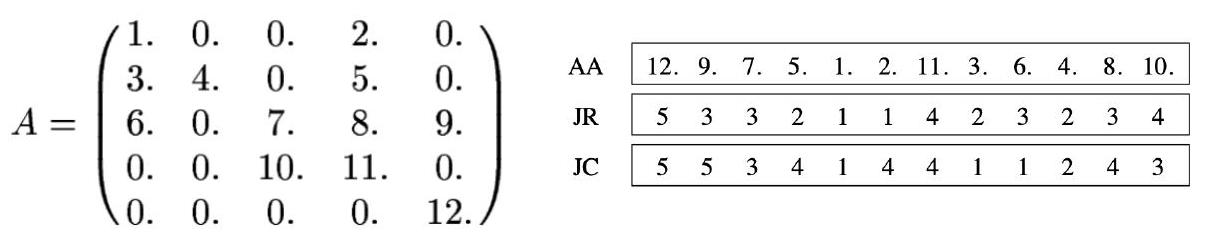
\includegraphics[max width=\textwidth]{2023_09_05_b72ccc85584d9dc6fb5cg-025}
\end{center}

\subsection*{Coordinate Compressed Sparse Row (CSR) format}
If the elements of $A$ are listed by row, the array JC might be replaced by an array that points to the beginning of each row.

\begin{itemize}
  \item AA: all the values of the nonzero elements of $A$, stored row by row from $1, \ldots, n$.

  \item JA: contains the column indices.

  \item IA: contains the pointers to the beginning of each row in the arrays $A$ and $J A$. Thus $I A(i)$ contains the position in the arrays AA and JA where the $i-$ th row starts. The length of IA is $n+1$, with $\mathrm{IA}(n+1)$ containing the number $\mathrm{A}(1)+\mathrm{nnz}(\mathrm{A})$.

\end{itemize}

\begin{center}
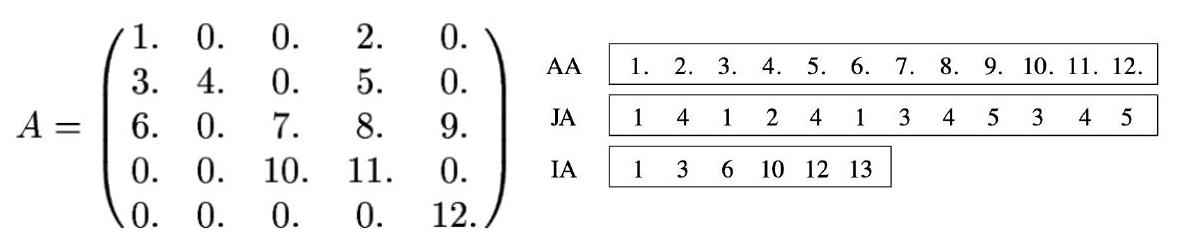
\includegraphics[max width=\textwidth]{2023_09_05_b72ccc85584d9dc6fb5cg-026}
\end{center}

\section*{Well-posed linear system}
A problem is well posed if it admits a unique solution  which depends with continuity on the data.\\ \\
Consider the linear system Ax $=\mathbf{b}$, where $\mathbf{x}$ and $\mathbf{b}$ are two vectors in $\mathbb{R}^n$, while $\mathbf{A}$ is the matrix $(n \times n)$ of the real coefficients of the system. Suppose that A is nonsingular; in such a case $x$ is the unknown solution $\mathbf{x}$, while the data $d$ are the right-hand side $\mathbf{b}$ and the matrix A, that is, $d=\left\{b_i, a_{i j}, 1 \leq i, j \leq n\right\}$.\\ 
If $\mathrm{A}$ is well conditioned, solving the linear system $\mathbf{A x}=\mathbf{b}$ is a stable problem with respect to perturbations of the right-hand side b. 


\newpage

\chapter{Iterative Methods}
In this chapter, we will study iterative methods for solving linear systems of equations, of the following form:
$$A \boldsymbol{x}=\boldsymbol{b}$$with, $A \in \mathbb{R}^{n \times n}$, $\boldsymbol{b} \in \mathbb{R}^{n}$ and $\boldsymbol{x} \in \mathbb{R}^{n}$.\\
In general, direct methods (i.e., methods based on a "manipulation" of $A$ ") are not suitable whenever:

\begin{itemize}
  \item $\quad n$ is large. Except for selected cases, the typical cost of direct methods scale as $n^{3}$.
  \item $A$ is sparse. Direct methods suffer from fill-in phenomenon (see later). Sparse matrices arise in many application problems, for example the approximation with Finite Elements or Finite Differences of partial differential equations.
\end{itemize}

\section*{Definition of a sparse matrix A}
Let $A \in \mathbb{R}^{n \times n}$, we say that $A$ is sparse the number of non-zero elements $(n n z(A))$ is roughly equal to the number of rows/columns $n$, i.e. $\mathrm{nnz}(\mathrm{A}) \sim n$

\begin{center}
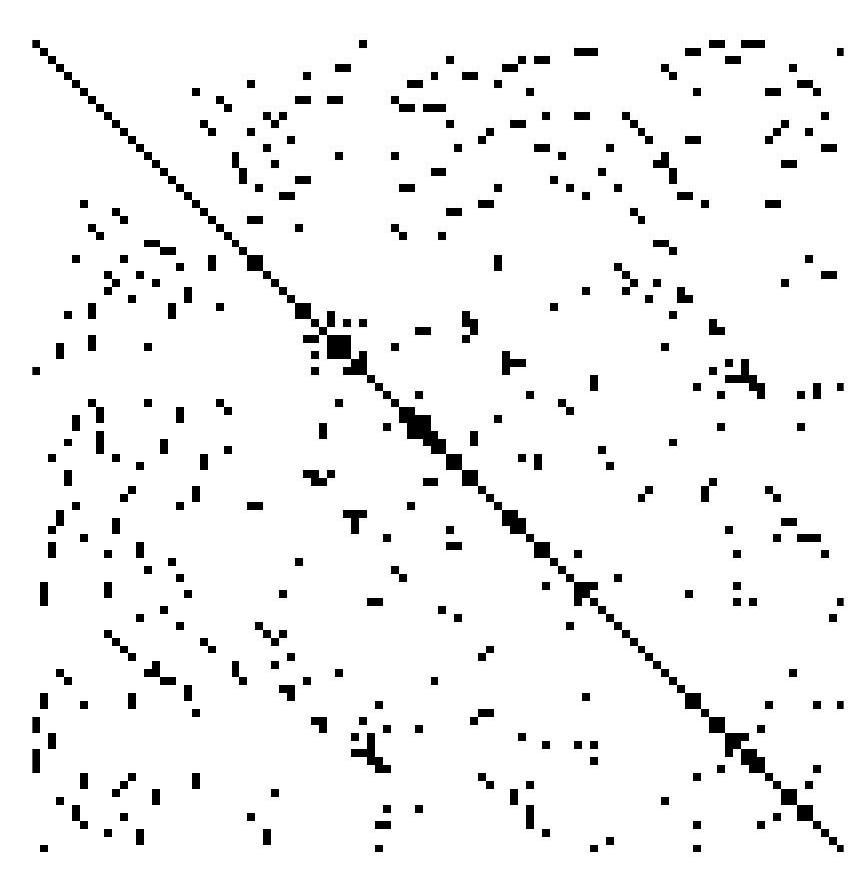
\includegraphics[scale = 0.22,max width=\textwidth]{2023_09_05_b72ccc85584d9dc6fb5cg-030}
\end{center}
A sparse matrix obtained when solving a finite element problem in two dimensions. The non-zero elements are shown in black.
\section*{Example of a sparse matrix systems}
Let us consider the following differential problem:
$$
\begin{cases}
& -u^{\prime \prime}(x)=f(x) \quad x \in(0,1) \\
& u(0)=u(1)=0
\end{cases}
$$
which describes (for example) the displacement of an elastic body constrained to the extremes under the action of a force $f(x)$.
\begin{center}
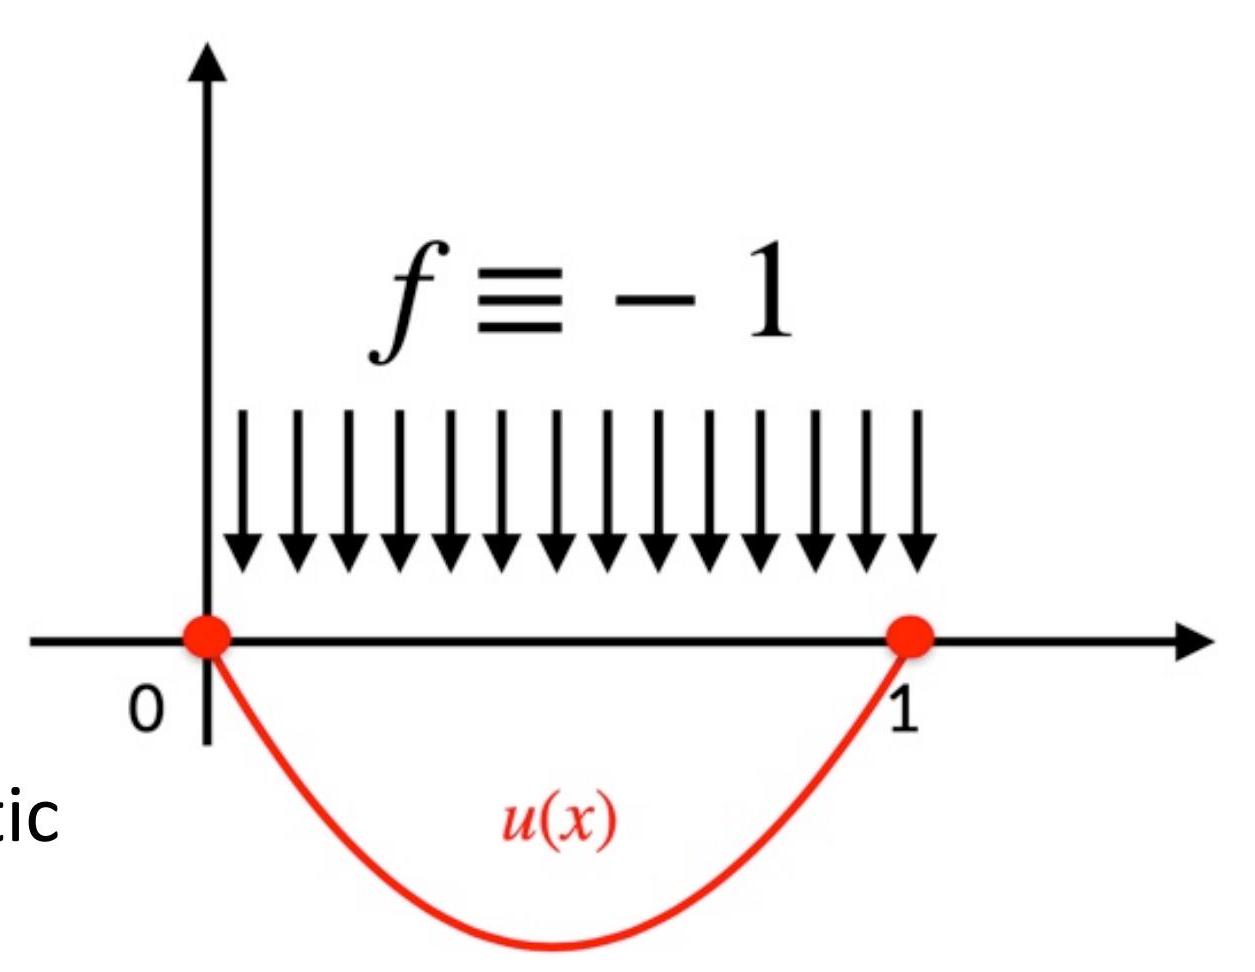
\includegraphics[scale = 0.2,max width=\textwidth]{2023_09_05_b72ccc85584d9dc6fb5cg-032(1)}
\end{center}

\textbf{Computational domain discretization}.
\begin{center}
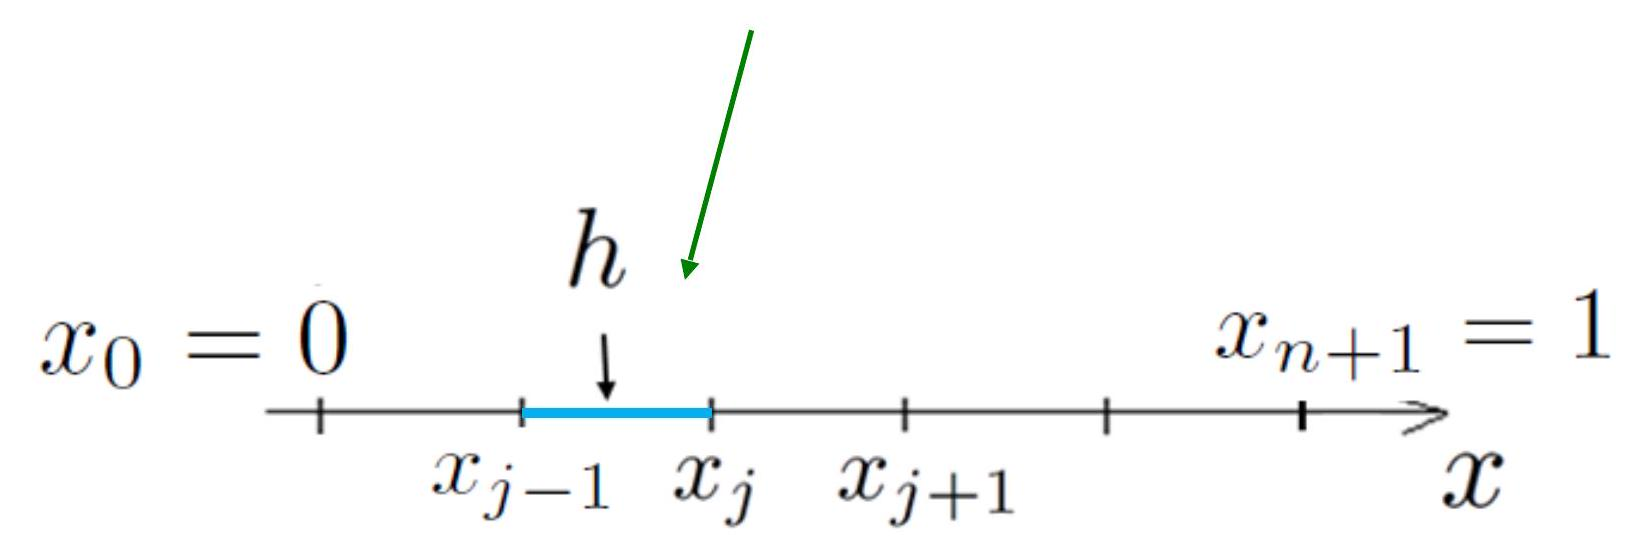
\includegraphics[max width=\textwidth]{2023_09_05_b72ccc85584d9dc6fb5cg-032}
\end{center}
In each node $x_{j}$ we can write the following approximate problem, obtained by approximating the second
derivative and introducing the numerical solution $u_{j}$
$$
-\frac{u_{j+1}-2 u_{j}+u_{j-1}}{h}=f\left(x_{j}\right)
$$
It is easy to verify that the previous set of equations is a linear system:
$$
A=\left(\begin{array}{cccccc}
2 & -1 & 0 & 0 & \cdots & 0 \\
-1 & 2 & -1 & 0 & \cdots & 0 \\
0 & -1 & 2 & -1 & \cdots & 0 \\
\vdots & \ddots & & \ddots & & \vdots \\
0 & \cdots & 0 & 0 & -1 & 2
\end{array}\right) \quad \mathbf{b}=h^{2}\left[\begin{array}{c}
f\left(x_{1}\right) \\
\vdots \\
f\left(x_{j}\right) \\
\vdots \\
f\left(x_{n}\right)
\end{array}\right]
$$

\section*{Definition of iterative methods}

We introduce a sequence $\mathbf{x}^{(k)}$ of vectors determined by a recursive relation that identifies the method.
In order to "initialise" the iterative process, it is necessary to provide a starting point (initial vector) $\mathbf{x}^{(0)}$ based, for example, on example on physical or engineering considerations: $\mathbf{x}^{(0)} \longrightarrow \mathbf{x}^{(1)} \longrightarrow \ldots \mathbf{x}^{(k)} \longrightarrow \mathbf{x}^{(k+1)} \longrightarrow \ldots$. \\
For the method to make sense, it must satisfy the convergence property:
$$
\lim _{k \rightarrow+\infty} \mathbf{x}^{(k)}=\mathbf{x}.
$$
Convergence must not depend on the choice of $\mathbf{x}^{(0)}$.

\section*{What do we expect from the accuracy of an iterative method?}
Since convergence is only guaranteed after an infinite number of iterations, from a practical point of view we will have to stop the iterative process after a finite number of iterations, when we believe we have arrived "sufficiently close" to the solution. \\
For the choice of specific stopping criteria, see below.\\


\section*{The Jacobi method}
Let's start from the $i$-th line of the linear system:

$$
\sum_{j=1}^{n} a_{i j} x_{j}=b_{i} \rightarrow a_{i 1} x_{1}+a_{i 2} x_{2}+\ldots+a_{i n} x_{n}=b_{i}
$$
Formally the solution $x_{i}$ for each $i$ is given by: $\quad x_{i}=\frac{b_{i}-\sum_{j \neq i} a_{i j} x_{j}}{a_{i i}}$.\\
Obviously the previous identity cannot be used in practice because we do not know $x_{j}$, for $j \neq i$.\\
However, we could think of introducing an iterative method that updates $x_{i}^{(k+1)}$ at step $k+1$ using the others $x_{j}^{(k)}$ obtained in the previous step $k$.
$$x_i^{(k+1)}=\frac{b_i-\sum_{j \neq i} a_{i j} x_j^{(k)}}{a_{i i}} \ \ \forall i=1, \ldots, n
$$
In general, each iteration costs $\sim n^{2}$ operations, so the Jacobi method is competitive if the number of iterations is less than $n$.\\
If $A$ is sparse matrix, then the cost is only $\sim n$ flops per iteration.\\
It should be noted that the solutions $x_{i}^{(k+1)}$ can be computed in a fully parallelized fashion.

 \section*{The Gauss Seidel method}
 Let's start from Jacobi's method:
$$
x_{i}^{(k+1)}=\frac{b_{i}-\sum_{j \neq i} a_{i j} x_{j}^{(k)}}{a_{i i}}
$$
At iteration $(k+1)$, let's consider the computation of $x_{i}^{(k+1)}$. We observe that for $j<i(i \geq 2), x_{j}^{(k+1)}$ is known (we have already calculated it). We can therefore think of using the quantities at step $(k+1)$ if $j<i$ and (as in the Jacobi method) those at the previous step $k$ if $j>i$:
$$
x_{i}^{(k+1)}=\frac{b_{i}-\sum_{j<i} a_{i j} x_{j}^{(k+1)}-\sum_{j>i} a_{i j} x_{j}^{(k)}}{a_{i i}}
$$
The computational costs are comparable to those of the Jacobi method.\\
Unlike Jacobi method, GS method is not fully parallelizable.

\section*{Linear iterative methods $\quad A \mathbf{x}=\mathbf{b}$}
In general, we consider linear iterative methods of the following form:
$$
\mathbf{x}^{(k+1)}=B \mathbf{x}^{(k)}+\mathbf{f} \quad k \geq 0
$$
where $B \in \mathbb{R}^{n \times n}, \mathbf{f} \in \mathbb{R}^{n}$.
$B$ is called iteration matrix. Its choice (together with that of $\mathbf{f}$ ) uniquely identify the method.
How to choose $B \in \mathbb{R}^{n \times n}, \mathbf{f} \in \mathbb{R}^{n}$ ?

\subsection*{Consistency}
If $\mathbf{x}^{(k)}$ is the exact solution $\mathbf{x}$, then $\mathbf{x}^{(k+1)}$ is again equal to $\mathbf{x}$ (no update if the exact solution is found).
$$
\boldsymbol{x}=B \boldsymbol{x}+\boldsymbol{f} \rightarrow \boldsymbol{f}=(I-B) \boldsymbol{x}=(I-B) A^{-1} \boldsymbol{b}
$$
The former identity gives a relationship between $B$ and $\mathbf{f}$ as a function of the data. It provides a necessary condition for convergence.
\subsection*{Convergence}
Let us introduce the error at step $(k+1): \mathbf{e}^{(k+1)}=\mathbf{x}-\mathbf{x}^{(k+1)}$ and a suitable vector norm $\|\cdot\|$ (for example the Euclidean norm). Then we have:
$$
\begin{aligned}
\left\|\boldsymbol{e}^{(k+1)}\right\| & =\left\|\boldsymbol{x}-\boldsymbol{x}^{(k+1)}\right\|=\left\|\boldsymbol{x}-B \boldsymbol{x}^{(k)}-\boldsymbol{f}\right\|=\longleftarrow \text { consistency } \\
& =\left\|\boldsymbol{x}-B \boldsymbol{x}^{(k)}-(I-B) \boldsymbol{x}\right\|=\left\|B \boldsymbol{e}^{(k)}\right\| \leq \\
& \leq\|B\|\left\|\boldsymbol{e}^{(k)}\right\|
\end{aligned}
$$
Note that $\|B\|$ is the matrix norm induced by the vector norm $\|\cdot\|$ By recursion we obtain

$$
\begin{aligned}
& \left\|\boldsymbol{e}^{(k+1)}\right\| \leq\|B\|\|B\|\left\|\boldsymbol{e}^{(k-1)}\right\| \leq \\
& \quad \leq\|B\|\|B\|\|B\|\left\|\boldsymbol{e}^{(k-2)}\right\| \leq \ldots \leq\|B\|^{k+1}\left\|\boldsymbol{e}^{(0)}\right\|
\end{aligned}
$$

$$
\lim _{k \rightarrow \infty}\left\|\boldsymbol{e}^{(k+1)}\right\| \leq\left(\lim _{k \rightarrow \infty}\|B\|^{k+1}\right)\left\|\boldsymbol{e}^{(0)}\right\|
$$
If $ ||B|| < 1 \implies \lim _{k \rightarrow \infty}\left\|\boldsymbol{e}^{(k+1)}\right\|=0
$. This is a sufficient condition for convergence.
$$
\rho(B)=\max _{j}\left|\lambda_{j}(B)\right|
$$
\textbf{Remark.} If $B$ is SPD, then $\rho(B)=\|B\|_{2}$.\\ \\
\textbf{Property.} Let $C \in \mathbb{R}^{n \times n}$ then $\rho(C)=\inf \{\|C\| \quad \forall$ induced matrix norm $\|\cdot\|\}$.\\ \\
From the aforementioned property, it follows that:
$$
\rho(B) \leq\|B\| \quad \forall \text { induced matrix norm }\|\cdot\|
$$
\textbf{Theorem (necessary and sufficient condition for convergence)}\\ \\
A consistent iterative method with iteration matrix B converges if and only if $\rho(B)<1$.\\ \\
\textbf{Remark.} Thanks to the same property we can observe that if:
$$
\exists\ \ ||\cdot|| \text { such that }\|B\|<1 \implies \rho(B)<1 \text { (and thus convergence). }
$$
Let
\begin{itemize}
  \item $D$ : the diagonal part of $A$
  \item $-E$ : lower triangular part of $A$
  \item $-F$ : upper triangular part of $A$
\end{itemize}
$$
A=\left[\begin{array}{ccc}
\ddots & & -F \\
& D & \\
-E & & \ddots
\end{array} \right].
$$
The Jacobi method can be rewritten as:
$$
D \boldsymbol{x}^{(k+1)}=(E+F) \boldsymbol{x}^{(k)}+\boldsymbol{b}
$$
Its iteration matrix is given by:
$$
B_{J}=D^{-1}(E+F)=D^{-1}(D-A)=I-D^{-1} A
$$
For the Gauss-Seidel method we have:
$$
(D-E) \boldsymbol{x}^{(k+1)}=F \boldsymbol{x}^{(k)}+\boldsymbol{b}
$$
The iteration matrix is given by:
$$
B_{G S}=(D-E)^{-1} F
$$
$$
A=\left[\begin{array}{ccc}
\ddots & & -F \\
& D & \\
-E & & \ddots
\end{array} \right].
$$
The proof that both method are consistent is left to the reader.\\ \\
\textbf{Theorem (sufficient condition for convergence)}\\
If $A$ is strictly diagonally dominant by rows, i.e.
$$
\left|a_{i i}\right|>\sum_{j \neq i}\left|a_{i j}\right|, i=1, \ldots, n,
$$
then J and GS method both converge.\\ \\
For the Jacobi method
\begin{center}
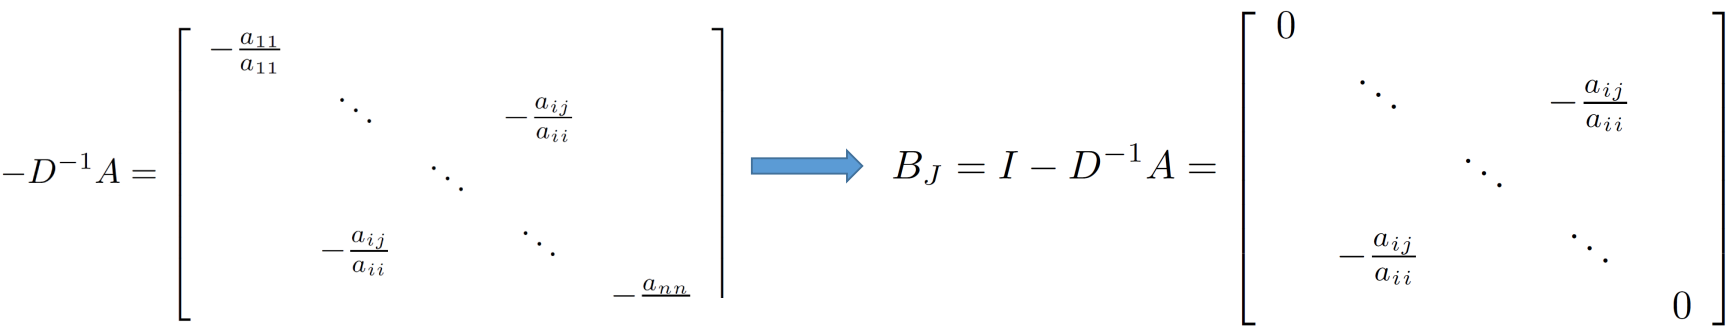
\includegraphics[scale=0.4]{images/Matrix1.png}
\end{center}
Taking the  following norm $\|C\|=\|C\|_{1}=\max _{i}\left(\sum_{j}\left|C_{i j}\right|\right)$, we obtain $\left\|B_{J}\right\|_{1}=\max _{i}\left(\sum_{j}\left|\left(B_{J}\right)_{i j}\right|\right)=\max _{i}\left(\sum_{j}\left|\frac{a_{i j}}{a_{i i}}\right|\right)$ from which it follows $\left\|B_{J}\right\|<1$, since $A$ is strictly diagonally.\\
\\
\textbf{Theorem (sufficient conditions for convergence)}
\begin{enumerate}
  \item If $A$ is strictly diagonally dominant by columns, then J e GS methods converge.\\
  \item If $A$ is SPD then the GS method converge.\\
  \item If $A$ is tridiagonal it can be shown that: $\rho^{2}\left(B_{J}\right)=\rho\left(B_{G S}\right)$. Therefore both methods converge or fail to converge at the same time. In this case GS method is more rapidly convergent than the J method.\\
\end{enumerate}

\section*{Stopping Criteria}
A stopping criteria is just a  practical test needed to determine when to stop the iteration. The idea is to terminate the iterations when: $ \frac{|| \boldsymbol{x}-\boldsymbol{x}^k}{||\boldsymbol{x}||} \leq \boldsymbol{\varepsilon}$.
Where $\boldsymbol{\varepsilon}$ is the user-defined tolerance. Unfortunately, we can't use this strategy in practice, since it would require the knowledge of the exact solution, which we are trying to find.
\begin{enumerate}
  \item Residual-based stopping criterion.
\end{enumerate}
This stopping criterion consists of continuing the iteration until $\left\|\mathbf{r}^{(k)}\right\| \leq \varepsilon, \varepsilon$ being a fixed tolerance. Note that:
$$
\left\|\mathbf{x}-\mathbf{x}^{(k)}\right\|=\left\|\mathrm{A}^{-1} \mathbf{b}-\mathbf{x}^{(k)}\right\|= || A^{-1}\mathbf{b}-\bigl(A^{-1}\mathbf{b}-A^{-1}\mathbf{r}^{k} \bigl) || = \left\|\mathrm{A}^{-1} \mathbf{r}^{(k)}\right\| \leq\left\|\mathrm{A}^{-1}\right\| \varepsilon
$$
Considering instead a normalized residual, i.e. stopping the iteration as soon as $\left\|\mathbf{r}^{(k)}\right\| /\|\mathbf{b}\| \leq \varepsilon$, we obtain the following control on the relative error:
$$
\frac{\left\|\mathbf{x}-\mathbf{x}^{(k)}\right\|}{\|\mathbf{x}\|} \leq \frac{\left\|\mathrm{A}^{-1}\right\|\left\|\mathbf{r}^{(k)}\right\|}{\|\mathbf{x}\|} = \frac{||A^{-1}|| ||\mathbf{r}^{k}||}{|| \mathbf{x} ||} \frac{||A||}{||A||} \leq K(A) \frac{||\mathbf{r}^{k}||}{||A\mathbf{x}||} \leq K(\mathrm{A}) \frac{\left\|\mathbf{r}^{(k)}\right\|}{\|\mathbf{b}\|} \leq \varepsilon K(\mathrm{~A}) .
$$
In the case of preconditioned methods, the residual is replaced by the preconditioned residual, so that the previous criterion becomes
$$
\frac{\left\|\mathrm{P}^{-1} \mathbf{r}^{(k)}\right\|}{\left\|\mathrm{P}^{-1} \mathbf{r}^{(0)}\right\|} \leq \varepsilon
$$
where $\mathrm{P}$ is the preconditioning matrix.
$$
\frac{\left\|\boldsymbol{x}-\boldsymbol{x}^{(k)}\right\|}{\|\boldsymbol{x}\|} \leq K(A) \frac{\left\|\boldsymbol{r}^{(k)}\right\|}{\|\boldsymbol{b}\|} \Longrightarrow \frac{\left\|\boldsymbol{r}^{(k)}\right\|}{\|\boldsymbol{b}\|} \leq \varepsilon
$$
Good stopping criterion whenever $K(A)$ is "small".
Usually employed for preconditioned scheme.
$$
\frac{\left\|\boldsymbol{x}-\boldsymbol{x}^{(k)}\right\|}{\|\boldsymbol{x}\|} \leq K\left(P^{-1} A\right) \frac{\left\|\boldsymbol{z}^{(k)}\right\|}{\|\boldsymbol{b}\|} \Longrightarrow \frac{\left\|\boldsymbol{z}^{(k)}\right\|}{\|\boldsymbol{b}\|} \leq \varepsilon \quad \boldsymbol{z}^{(k)}=P^{-1} \boldsymbol{r}^{(k)}
$$
\begin{enumerate}
  \setcounter{enumi}{1}
  \item Distance between consecutive iterates. Define $\boldsymbol{\delta}^{(k)}=\mathbf{x}^{(k+1)}-\mathbf{x}^{(k)}$
\end{enumerate}
$$
\left\|\boldsymbol{\delta}^{(k)}\right\| \leq \varepsilon
$$
It can be shown that: $\left\|\mathbf{e}^{(k)}\right\| \leq \frac{1}{1 -\rho(\mathrm{B})}\left\|\boldsymbol{\delta}^{(k)}\right\| $.\\ \\
There is a relationship between the true error and $\boldsymbol{\delta}^{(k)}$:
$$\begin{aligned}\left\|\boldsymbol{e}^{(k)}\right\| & =\left\|\boldsymbol{x}-\boldsymbol{x}^{(k)}\right\|=\left\|\boldsymbol{x}-\boldsymbol{x}^{(k+1)}+\boldsymbol{x}^{(k+1)}-\boldsymbol{x}^{(k)}\right\|= \\ & =\left\|\boldsymbol{e}^{(k+1)}+\boldsymbol{\delta}^{(k)}\right\| \leq \rho(B)\left\|\boldsymbol{e}^{(k)}\right\|+\left\|\boldsymbol{\delta}^{(k)}\right\|\end{aligned}$$
Therefore this is a "good" stopping criterion only if $\rho(B)<<1$.
\subsection*{Example: Gauss-Seidel method, Hilbert matrix.}
\begin{center}
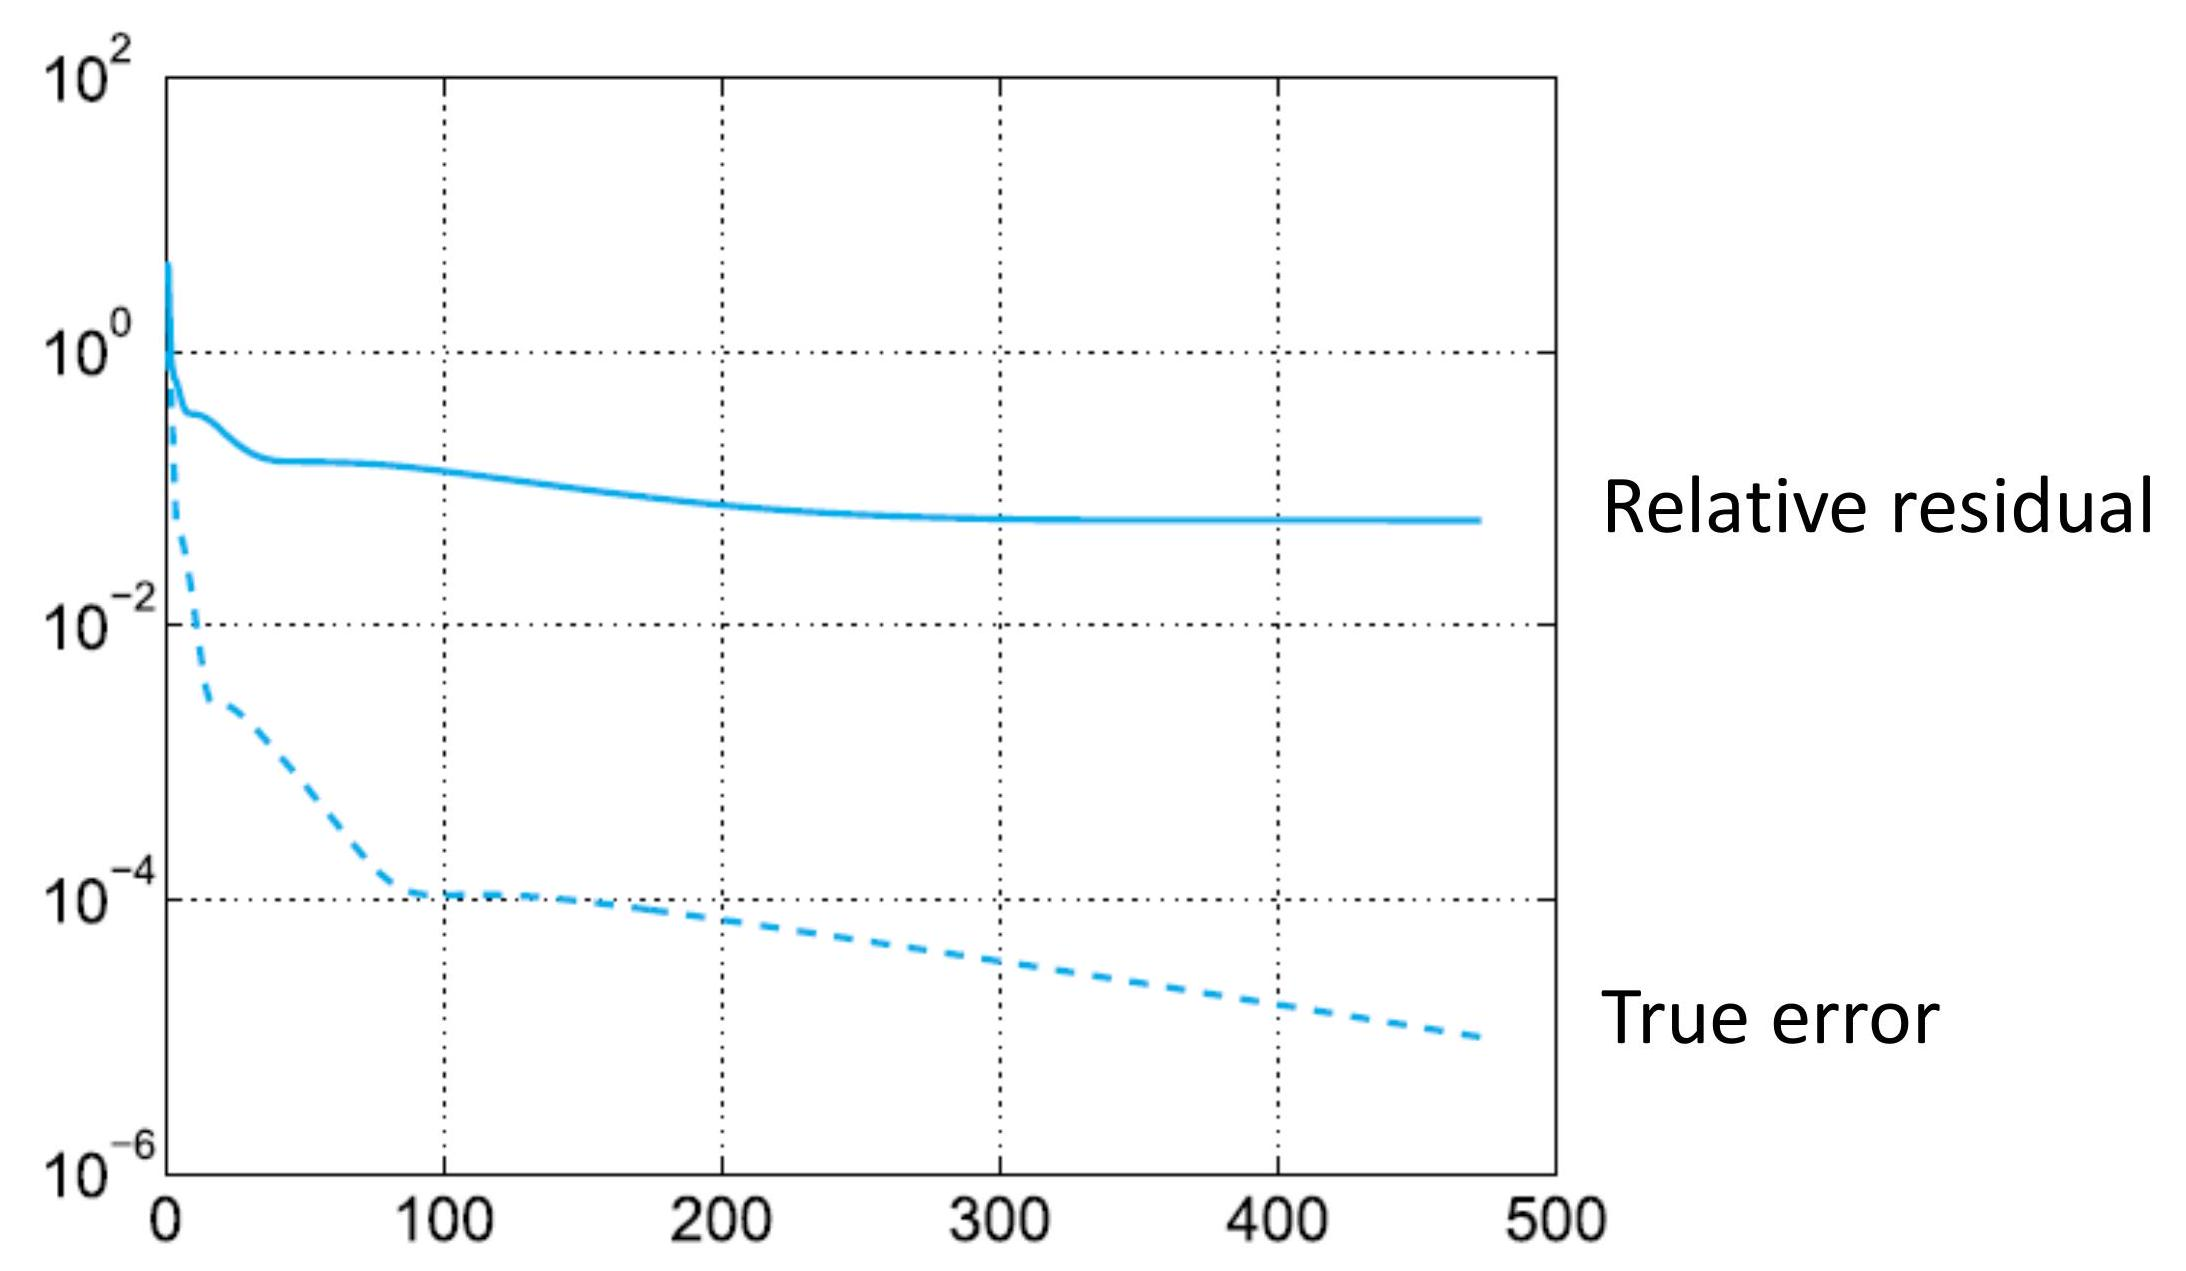
\includegraphics[max width=\textwidth]{2023_09_05_b72ccc85584d9dc6fb5cg-054}
\end{center}

\section*{The stationary Richardson method}
Given $\mathbf{x}^{(0)} \in \mathbb{R}^{n}, \alpha \in \mathbb{R}$, It is based on the following recursive update:
$$
\boldsymbol{x}^{(k+1)}=\boldsymbol{x}^{(k)}+\alpha \underbrace{\left(\boldsymbol{b}-A \boldsymbol{x}^{(k)}\right)}_{\text { residual } \boldsymbol{r}^{(k)}}
$$
The idea is to update the numerical solution by adding a quantity proportional to the residual. Indeed, it is expected that if the residual is "large" ("small"), the solution at step $k$ should be corrected "a lot"( "slightly").\\
From (2) it follows $\mathbf{x}^{(k+1)}=(I-\alpha A) \mathbf{x}^{(k)}+\alpha \mathbf{b}$.\\
Therefore, the stationary Richardson method is characterised by the iteration matrix $B_{\alpha}=I-\alpha A$ and by $\mathbf{f}=\alpha \mathbf{b}$.
The stationary Richardson method is consistent, indeed:
$$
B_{\alpha}=I-\alpha A \quad \mathbf{x}=\mathbf{x}+\alpha(\mathbf{b}-A \mathbf{x})
$$
Let $A$ be the SPD
We introduce the eigenvalues of $A$ (which are real and positive):
$$
\lambda_{\max }(A)=\lambda_{1}(A) \geq \lambda_{2}(A) \geq \ldots \geq \lambda_{n}(A)=\lambda_{\min }(A)>0
$$
\textbf{Theorem}: Let $A$ be a symmetric and positive definite matrix. The stationary Richardson method is convergent if and only if
$$
0<\alpha<\frac{2}{\lambda_{\max }(A)}
$$
\textbf{Sketch of the proof}.
$$
\lambda_{\max }(A)=\lambda_1(A) \geq \lambda_2(A) \geq \ldots \geq \lambda_n(A)=\lambda_{\min }(A)>0
$$
$$
0<\alpha<\frac{2}{\lambda_{\max }(A)}
$$
$$
\left\|\boldsymbol{e}^{(k+1)}\right\| \leq \rho\left(B_\alpha\right)\left\|\boldsymbol{e}^{(k)}\right\|
$$
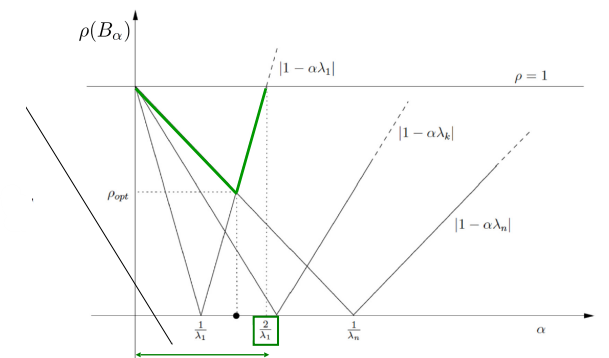
\includegraphics[scale=0.7]{images/Richardson0.png}\\
\textbf{Proof}\\
$\implies$ Let $\mu_i, i=1, \ldots, n$, be the eigenvalues of $B_\alpha=I-\alpha A$. We have:
$$
\mu_i=1-\alpha \lambda_i, i=1, \ldots, n
$$
To have convergence it must hold that $\left|1-\alpha \lambda_i(A)\right|<1, \ \forall i=1, \ldots, n$
$$
-1<1-\alpha \lambda_i(A)<1, \  \forall i=1, \ldots, n
$$
$$
0<\alpha \lambda_i(A)<2, \  \forall i=1, \ldots, n
$$
The first bound holds if $0<\alpha$
The second bound holds if
$$
\alpha<\frac{2}{\lambda_i(A)} \quad \forall i=1, \ldots, n
$$
$\impliedby$ Assume that $\alpha$ is not in the interval $(0, \frac{2}{\lambda_{\text{max}}(A)})$. This means that either $\alpha \leq 0$ or $\alpha \geq \frac{2}{\lambda_{\text{max}}(A)}$.
\begin{enumerate}
\item If $\alpha \leq 0$, then for all eigenvalues $\lambda(A)$ of $A$, we have $\alpha\lambda(A) \leq 0$. Subtracting $\alpha\lambda(A)$ from $1$ gives us $1 - \alpha\lambda(A) \geq 1$. Taking absolute values, we get $|1 - \alpha\lambda(A)| \geq 1$. Since $|1 - \alpha\lambda_i(A)|$ is the absolute value of the eigenvalues of $B_\alpha$, this implies that all eigenvalues of $B_\alpha$ are greater than or equal to $1$ in absolute value. Therefore, the spectral radius $\rho(B_\alpha)$, which is the maximum absolute value of its eigenvalues, satisfies $\rho(B_\alpha) \geq 1$. The spectral radius $\rho(B_\alpha) \geq 1$ means that the method does not converge.\\
\item If $\alpha \geq \frac{2}{\lambda_{\text{max}}(A)}$, then for the maximum eigenvalue $\lambda_{\text{max}}(A)$ of $A$, we have $\alpha\lambda_{\text{max}}(A) \geq 2$. Subtracting $\alpha\lambda_{\text{max}}(A)$ from $1$ gives us $1 - \alpha\lambda_{\text{max}}(A) \leq -1$. Taking absolute values, we get $|1 - \alpha\lambda_{\text{max}}(A)| \geq 1$. Since $|1 - \alpha\lambda_i(A)|$ is the absolute value of the eigenvalues of $B_\alpha$, this implies that at least one eigenvalue of $B_\alpha$ is greater than or equal to $1$ in absolute value. Therefore, the spectral radius $\rho(B_\alpha)$, which is the maximum absolute value of its eigenvalues, satisfies $\rho(B_\alpha) \geq 1$. The spectral radius $\rho(B_\alpha) \geq 1$ means that the method does not converge.
\end{enumerate}
Therefore, if $\alpha$ is not in the interval $(0, \frac{2}{\lambda_{\text{max}}(A)})$, then the stationary Richardson method does not converge $\square$\\

\subsection*{Choice of the optimal parameter $\alpha$}
We now ask ourselves what is the value of the parameter $\alpha$, among those that guarantee convergence, which maximises the speed of convergence.
We introduce the following A-induced norm (remember that $A$ is SPD).
$$
\|\boldsymbol{z}\|_{A}=\sqrt{\sum_{i, j=1}^{n} a_{i j} z_{i} z_{j}} \longleftrightarrow\|\boldsymbol{z}\|_{A}=\sqrt{(A \boldsymbol{z}, \boldsymbol{z})}=\sqrt{\boldsymbol{z}^{T} A \boldsymbol{z}}
$$
Recall that $\left\|\boldsymbol{e}^{(k+1)}\right\|_{A} \leq \rho\left(B_{\alpha}\right)\left\|\boldsymbol{e}^{(k)}\right\|_{A}$.\\
We look for $0<\alpha_{\text {opt }}<2 / \lambda_{\max (A)}$ such that $\rho\left(B_{\alpha}\right)$ is minimum. That is
$$
\alpha_{o p t}=\underset{0<\alpha<2 / \lambda_{\max }(A)}{\operatorname{argmin}}\left\{\max _{i}\left|1-\alpha \lambda_{i}(A)\right|\right\}
$$
We plot on the $\mathrm{x}$-axis the values of $\alpha$ and on the $\mathrm{y}$-axis $\left|1-\alpha \lambda_{i}(A)\right|, i=1 \ldots, n$.
The optimal value is given by the intersection between the curves $\left|1-\alpha \lambda_{1}(A)\right|$ and $\left|1-\alpha \lambda_{n}(A)\right|$.\\
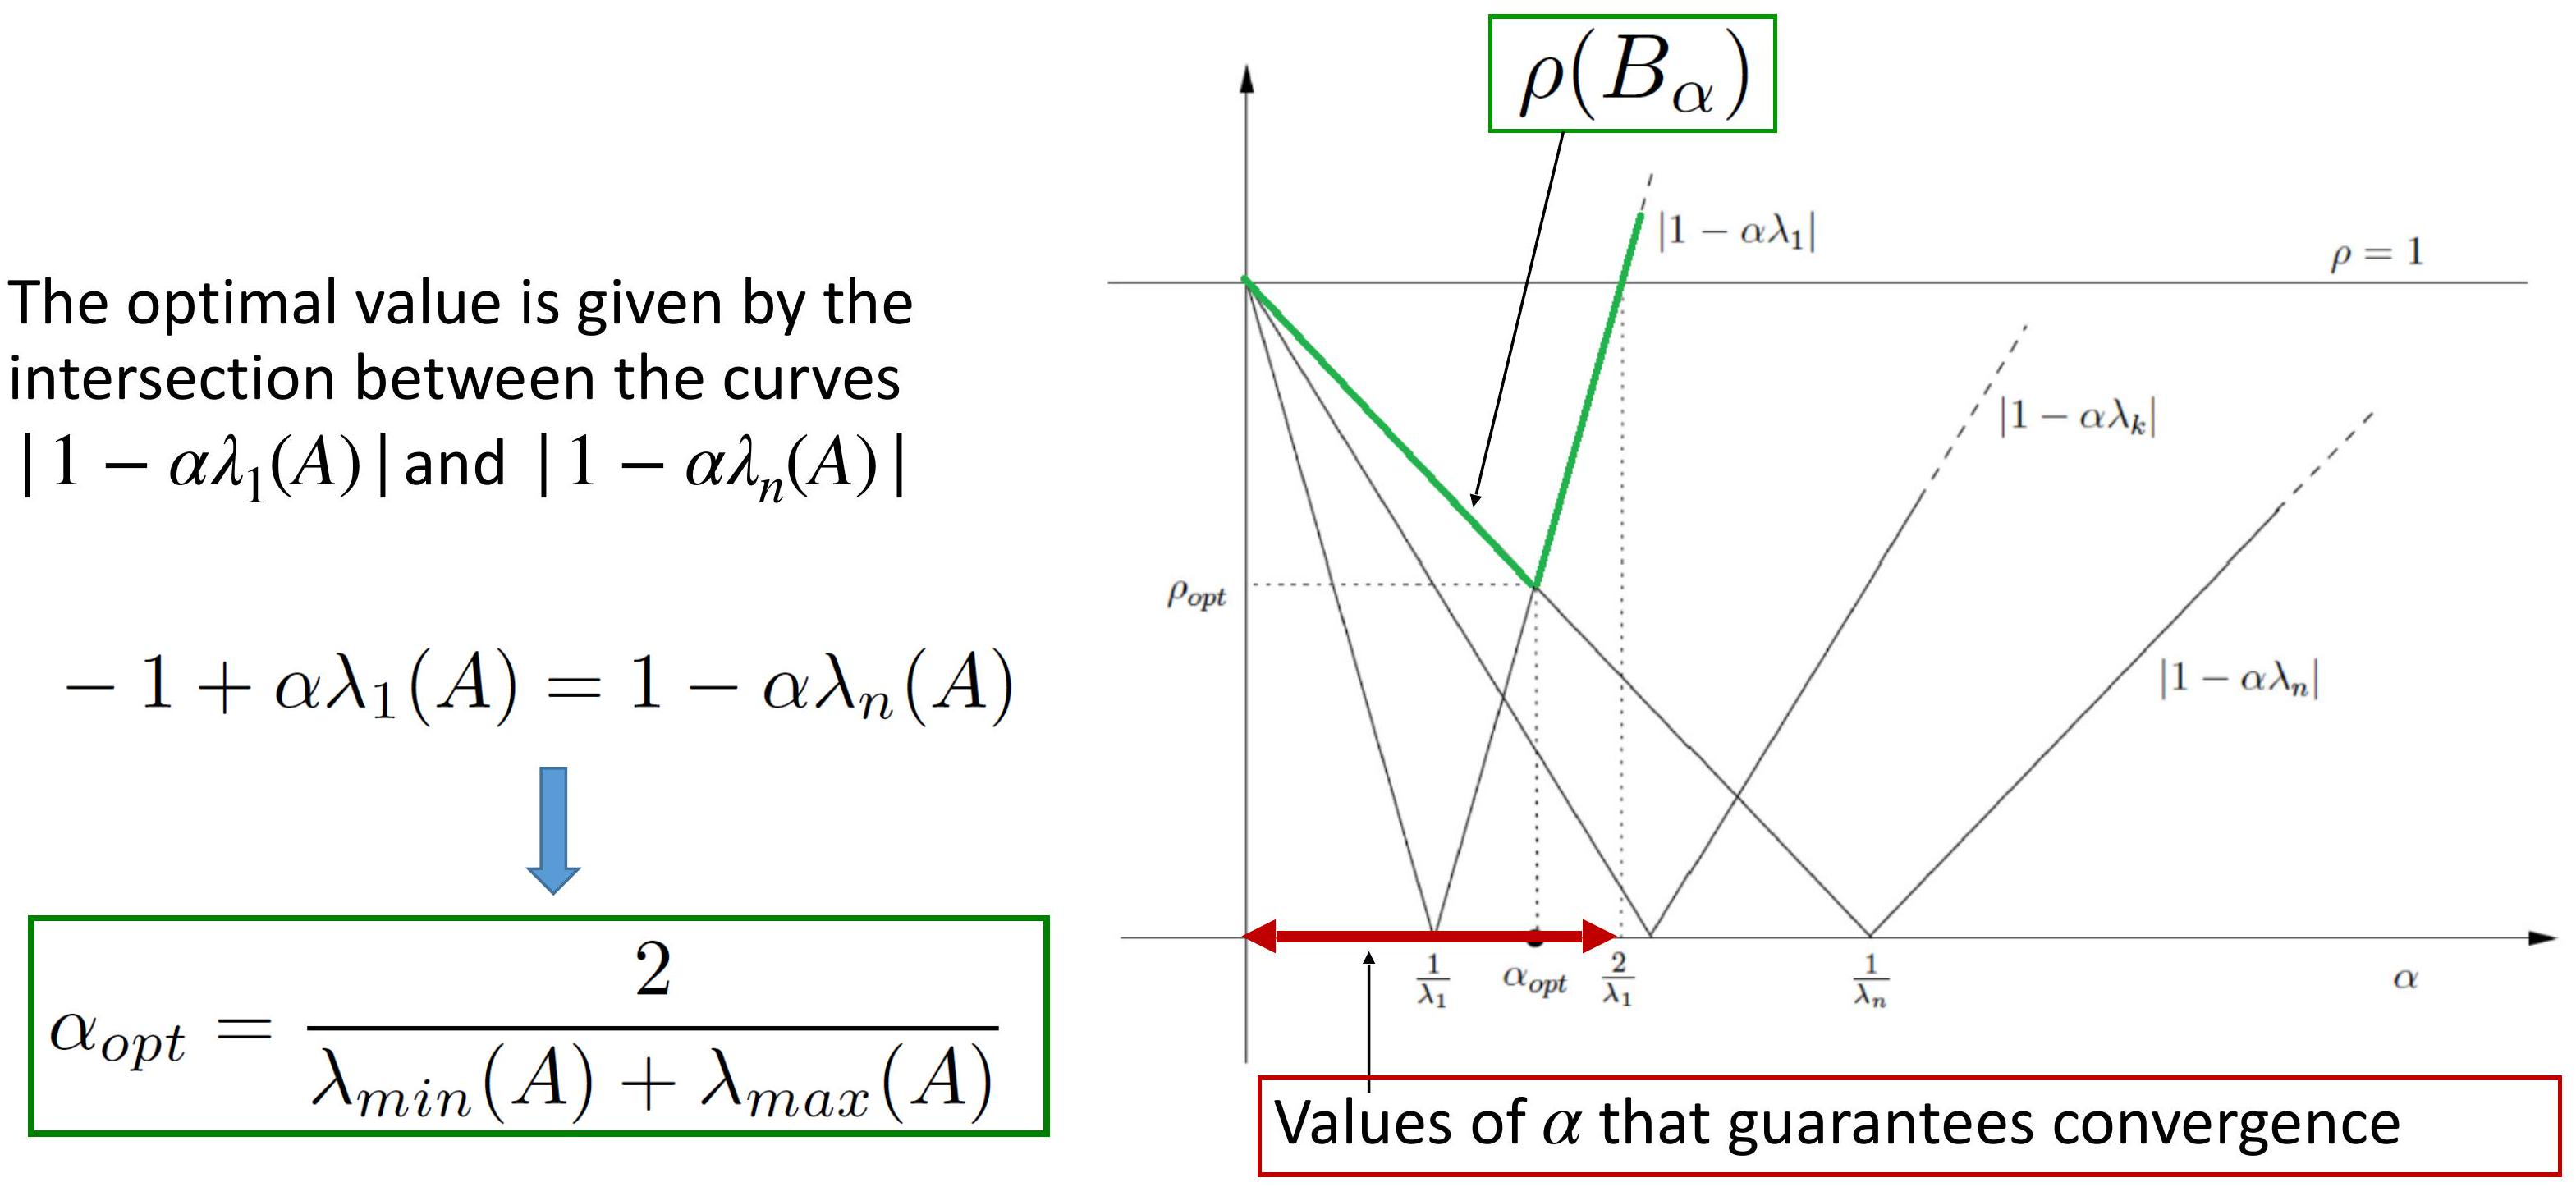
\includegraphics[max width=\textwidth, center]{2023_09_05_b72ccc85584d9dc6fb5cg-061}

\section*{Maximum convergence speed:}
We now calculate the value of the "optimal" spectral radius $\rho_{\mathrm{opt}}$, at the value of the optimal parameter $\alpha_{\mathrm{opt}}$:
$$
\begin{aligned}
\rho_{\text {opt }}=\rho\left(B_{\alpha_{\text {opt }}}\right)= & -1+\alpha_{\text {opt }} \lambda_{\max }(A)=1-\alpha_{\text {opt }} \lambda_{\min }(A)= \\
& =\frac{\lambda_{\max }(A)-\lambda_{\min }(A)}{\lambda_{\max }(A)+\lambda_{\min }(A)}
\end{aligned}
$$
Since $A$ is SPD, we have $\|A\|_2=\lambda_{\max }(A)$. Moreover, $\lambda_i\left(A^{-1}\right)=1 / \lambda_i(A), \forall i=1, \ldots, n$
$$
\rho_{\text {opt }}=\frac{K(A)-1}{K(A)+1}
$$


\section*{Preconditioning techniques}
\subsection*{Condition number and speed of convergence:}
The optimal value $\rho_{\text {opt }}=\frac{K(A)-1}{K(A)+1}$ expresses the maximum convergence speed that can be attained with a Stationary Richardson method.\\
Badly conditioned matrices $(K(A)>>1)$ are characterised by a very low convergence rate. How can we improve the speed of convergence?\\ \\
IDEA. We introduce a SDP matrix $P^{-1}$ (the so called preconditioner). Then, solving $A \mathbf{x}=\mathbf{b}$ is equivalent to the following preconditioned system:
$$
P^{-1 / 2} A P^{-1 / 2} \mathbf{z}=P^{-1 / 2} \mathbf{b}
$$
where $\mathbf{x}=P^{-1 / 2} \mathbf{z}$.\\ \\
\textbf{Rule of Thumb}. Choose $P^{-1}$ such that $K\left(P^{-1 / 2} A P^{-1 / 2}\right)<<K(A)$ Suppose that $P^{-1} A$ has real and positive eigenvalues. We apply the stationary Richardson method to $P^{-1} A$, i.e.,
$$
\boldsymbol{x}^{(k+1)}=\boldsymbol{x}^{(k)}+\alpha P^{-1}\left(\boldsymbol{b}-A \boldsymbol{x}^{k}\right)=\boldsymbol{x}^{(k)}+\alpha P^{-1} \boldsymbol{r}^{(k)}
$$
We obtain the same convergence results as in the non-preconditioned case, provided we replace $A$ with $P^{-1} A$. \\
Convergence:
$$
0<\alpha<\frac{2}{\lambda_{\max }\left(P^{-1} A\right)}
$$
Optimal values:
$$
\begin{aligned}
& \alpha_{o p t}=\frac{2}{\lambda_{\min }\left(P^{-1} A\right)+\lambda_{\max }\left(P^{-1} A\right)} \\
& \rho_{\text {opt }}=\frac{K\left(P^{-1} A\right)-1}{K\left(P^{-1} A\right)+1}
\end{aligned}
$$
Therefore, if $K\left(P^{-1} A\right)<<K(A)$ we obtain a higher convergence rate with respect to the non-preconditioned case.
$$
\rho_{o p t}=\frac{K\left(P^{-1} A\right)-1}{K\left(P^{-1} A\right)+1}
$$\\
Can we therefore say that such a preconditioned method is faster than the no preconditioned case? No!\\
For the moment we can only say that the number of iterations \#Iterneeded to satisfy a certain stopping criterion is lower in the preconditioned case than in the un-reconditioned one.\\ \\
Indeed, the CPU time is given by:
$$
\mathrm{CPU} \text { time }=\# \text { Iter } \times C.
$$
Remember that $\boldsymbol{x}^{(k+1)}=\boldsymbol{x}^{(k)}+\alpha P^{-1} \boldsymbol{r}^{(k)}$.\\
We defined the preconditioned residual: $\boldsymbol{z}^{(k)}=P^{-1} \boldsymbol{r}^{(k)}$.\\ \\
\textbf{Pseudo-algorithm.}\\
For any $k=0,1,2,3, \ldots$.
\begin{enumerate}
\item Compute $\alpha_{\text{opt}}=\frac{2}{\lambda_{\min}\left(P^{-1} A\right)+\lambda_{\max}\left(P^{-1} A\right)}$
\item Update $\boldsymbol{r}^{(k)}=\boldsymbol{b}-A \boldsymbol{x}^{(k)}$
\item Solve $P \boldsymbol{z}^{(k)}=\boldsymbol{r}^{(k)}$
\item Update $\boldsymbol{x}^{(k+1)}=\boldsymbol{x}^{(k)}+\alpha_{\text{opt}} \boldsymbol{z}^{(k)}$
\end{enumerate}
In the third step we have to solve a linear system in P. We need
$$
K\left(P^{-1} A\right)<<K(A)
$$
Using a preconditioner $P$ can help reduce the number of iterations required for convergence in iterative methods. The preconditioner should be chosen such that the eigenvalues of $P^{-1}A$ are clustered, and the linear system involving $P$ can be easily solved. To achieve this, $P$ should have a special structure, like block diagonal or block triangular.\\
When $P$ is easy to invert, the condition number of $P^{-1}A$ is approximately equal to the condition number of $A$, as shown below:
$$
\begin{gathered}
K\left(P^{-1} A\right) \simeq K(A) \\
\end{gathered}
$$
When $P$ is difficult to invert, the condition number of $P^{-1}A$ is much smaller than the condition number of $A$, as shown below:
$$
{K\left(P^{-1} A\right)<<K(A)}
$$
This approach is particularly useful for linear systems with sparse matrices. \\
\textbf{How should the preconditioner be chosen?}
\begin{equation}
\text{CPU time} = \text{\#Iter} \times C
\end{equation}
We need:
\begin{equation}
K(P^{-1}A) << K(A)
\end{equation}
As seen, this allows us to reduce \#Iter. To this end, the preconditioner $P$ should be chosen such that $P^{-1}A$ have clustered eigenvalues. \\
The linear system in $P$ must be "easily solved".\\
This allows to have $C$ not too large. To this aim, $P$ should have a special structure, for example, $P$ (block) diagonal, (block) triangular.\\ \\
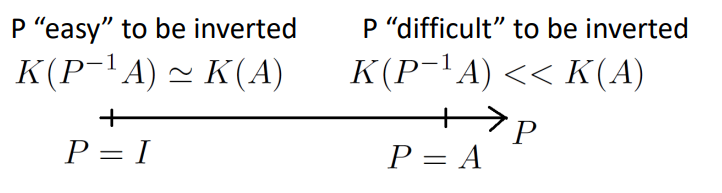
\includegraphics[scale=0.7]{images/Arrow.png}


\subsection*{Inexact LU factorization}

In the case of Inexact LU factorization, we take $P_{ILU}=\widetilde{L} \widetilde{U}$, where $\widetilde{L}$ and $\widetilde{U}$ are the incomplete $L$ and $U$ factors, i.e., $A \approx \widetilde{L} \widetilde{U}$ with $\widetilde{\ell}_{ij}=0$ and $\widetilde{u}_{ij}=0$ if $\widetilde{a}_{ij}=0$. This ensures that the factors $\widetilde{L}$ and $\widetilde{U}$ have the same sparsity pattern as $A$, and therefore, the memory occupation is the same (no fill-in). Although $A \neq \widetilde{L} \widetilde{U}$, the idea is to use incomplete LU factorization as a preconditioner because it contains information about $A$ and is easy to compute the action of the preconditioner (incomplete LU factorization + 2 triangular systems $\sim n^2$ FLOPS). An example of this is the inexact LU factorization applied to a sparse matrix $A$ and its incomplete $\tilde{L}$ and $\tilde{U}$ factors.
\section*{The Gradient Method}
In the upcoming discussion, we're going to make some assumptions about a matrix $A$. We'll assume that $A$ is a real-valued matrix (meaning its entries are real numbers) with a dimension of $n$, where $n$ is any integer greater than or equal to 1. 
Furthermore, we're assuming that $A$ is both symmetric (meaning it's equal to its own transpose, or $A=A^{T}$) and positive definite. A positive definite matrix is one where, for any non-zero vector $\mathbf{y}$ in $\mathbb{R}^{n}$, the result of $\mathbf{y}^{T} A \mathbf{y}$ is always greater than zero.
With these assumptions in place, we can say that solving the linear system represented by the equation $A \mathbf{x}=\mathbf{b}$ is the same as minimizing the quadratic function $\Phi$. This function, which maps from $\mathbb{R}^{n}$ to $\mathbb{R}$, is defined as follows:
$$
\Phi(\mathbf{y})=\frac{1}{2} \mathbf{y}^{T} A \mathbf{y}-\mathbf{y}^{T} \mathbf{b}
$$
In simpler terms, to solve our linear system, we need to find the vector $\mathbf{y}$ that makes $\Phi(\mathbf{y})$ as small as possible.\\ \\
As $A$ is positive definite, the hyperplane given by $\mathbf{z}=\Phi(\mathbf{y})$ defines a paraboloid in $\mathbb{R}^{n+1}$ with $n$-dimensional ellipsoids as iso-surfaces $\Phi(\mathbf{y})=$ const. and $\Phi(\cdot)$ has a global minimum in $\mathbf{x}$ (the equivalence of the problems is obvious, see later). Remember that $A$ is SPD. We introduce the following energy function $\Phi: \mathbb{R}^{n} \longrightarrow \mathbb{R}$.
$$
\Phi(\mathbf{y})=\frac{1}{2} \mathbf{y}^{T} A \mathbf{y}-\mathbf{y}^{T} \mathbf{b}
$$
If $A$ is SDP, the energy is a convex function that admits a unique minimum.\\
Since $\nabla \Phi(\mathbf{y})=A \mathbf{y}-\mathbf{b}$ we have that the minimum ( $\nabla \Phi(\mathbf{x})=\mathbf{0})$ coincides with the solution of $A \mathbf{x}-\mathbf{b}$.
\begin{center}
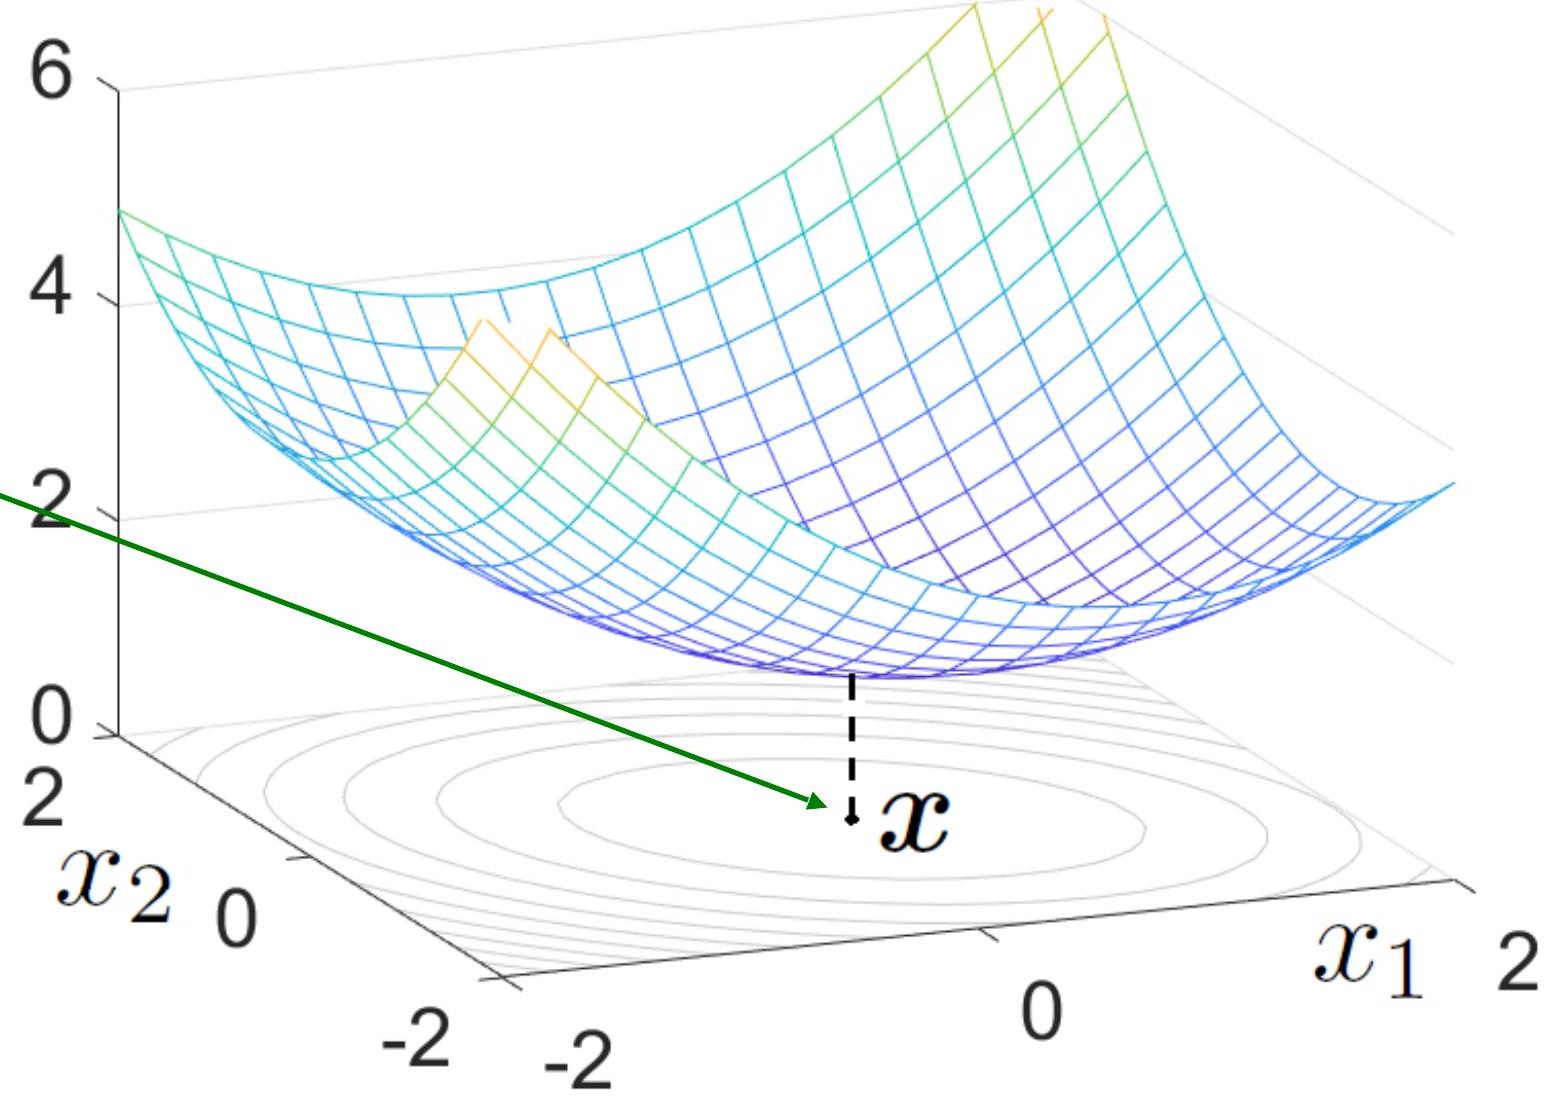
\includegraphics[scale = 0.7,max width=\textwidth]{2023_09_05_b72ccc85584d9dc6fb5cg-073}
\end{center}
\subsection*{A simple 2D example}
$$\left[\begin{array}{ll}2 & 0 \\ 0 & 1\end{array}\right]\left[\begin{array}{l}x \\ y\end{array}\right]=\left[\begin{array}{l}0 \\ 0\end{array}\right]$$ \\
This is equivalent to minimizing the quadratic function $\Phi(x, y)=x^{2}+\frac{1}{2} y^{2}$.

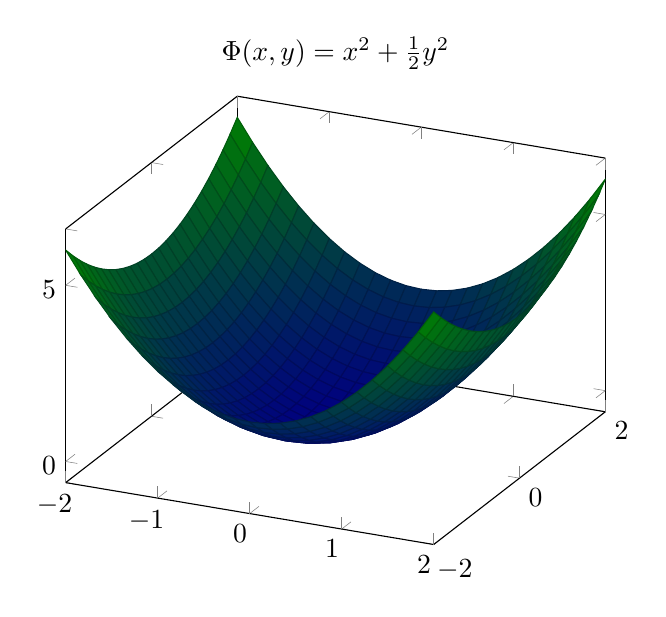
\begin{tikzpicture}  
\begin{axis}[  
    title={$\Phi(x, y)=x^{2}+\frac{1}{2} y^{2}$},  
    domain=-2:2,  
    y domain=-2:2,  
    colormap={bluegreen}{rgb255(0cm)=(0,0,128); rgb255(1cm)=(0,128,0)}  
]  
\addplot3[surf] {x^2+0.5*y^2};  
\end{axis}  
\end{tikzpicture}  
\hspace{1cm}  
\begin{tikzpicture}  
\begin{axis}[  
    title={Isolines for $\Phi(x, y)$},  
    view={0}{90},  
    domain=-2:2,  
    y domain=-2:2,  
    axis lines=middle,  
    colormap={bluegreen}{rgb255(0cm)=(0,0,128); rgb255(1cm)=(0,128,0)}  
]  
\addplot3[contour gnuplot={number=10}, thick] {x^2+0.5*y^2};  
\end{axis}  
\end{tikzpicture} \\
Every perturbation $\mathbf{e} \neq \mathbf{0}$ of the solution $\mathbf{x}$ of $A \mathbf{x}=\mathbf{b}$ increases the value of $\Phi(\mathbf{x})$.
$$
\Phi(\mathbf{x}+\mathbf{e})=\ldots=\Phi(\mathbf{x})+\frac{1}{2} \mathbf{e}^{T} A \mathbf{e}>\Phi(\mathbf{x})
$$
A possibility to find the minimum $\mathbf{x}$ is provided by the method of steepest descent.

\subsection*{Steepest descent}
The method of steepest descent tries to find an update $\mathbf{x}^{(k+1)}$ in the direction of the steepest descent of our quadratic function, i.e., in the direction of the negative gradient.
$$-\nabla \Phi\left(\mathbf{x}^{(k)}\right)= - \biggl( \frac{1}{2} \bigl(A^{T} +A \bigl) \mathbf{x}^{(k)} - \mathbf{b} \biggl) =  \mathbf{b}-A \mathbf{x}^{(k)}=\mathbf{r}^{(k)}.$$
\textbf{Remark}: It would be better  to search in the direction of the error $\mathbf{e}^{(k)}=\mathbf{x}-\mathbf{x}^{(k)}$, but unfortunately the error is unknown. Indeed, for a given $\overline{\mathbf{x}}$, the vector $-\nabla 
\Phi(\overline{\mathbf{x}})=\overline{\mathbf{r}}$ is the direction of steepest descent, orthogonal to the energy isoline at $\overline{\mathbf{x}}$.\\
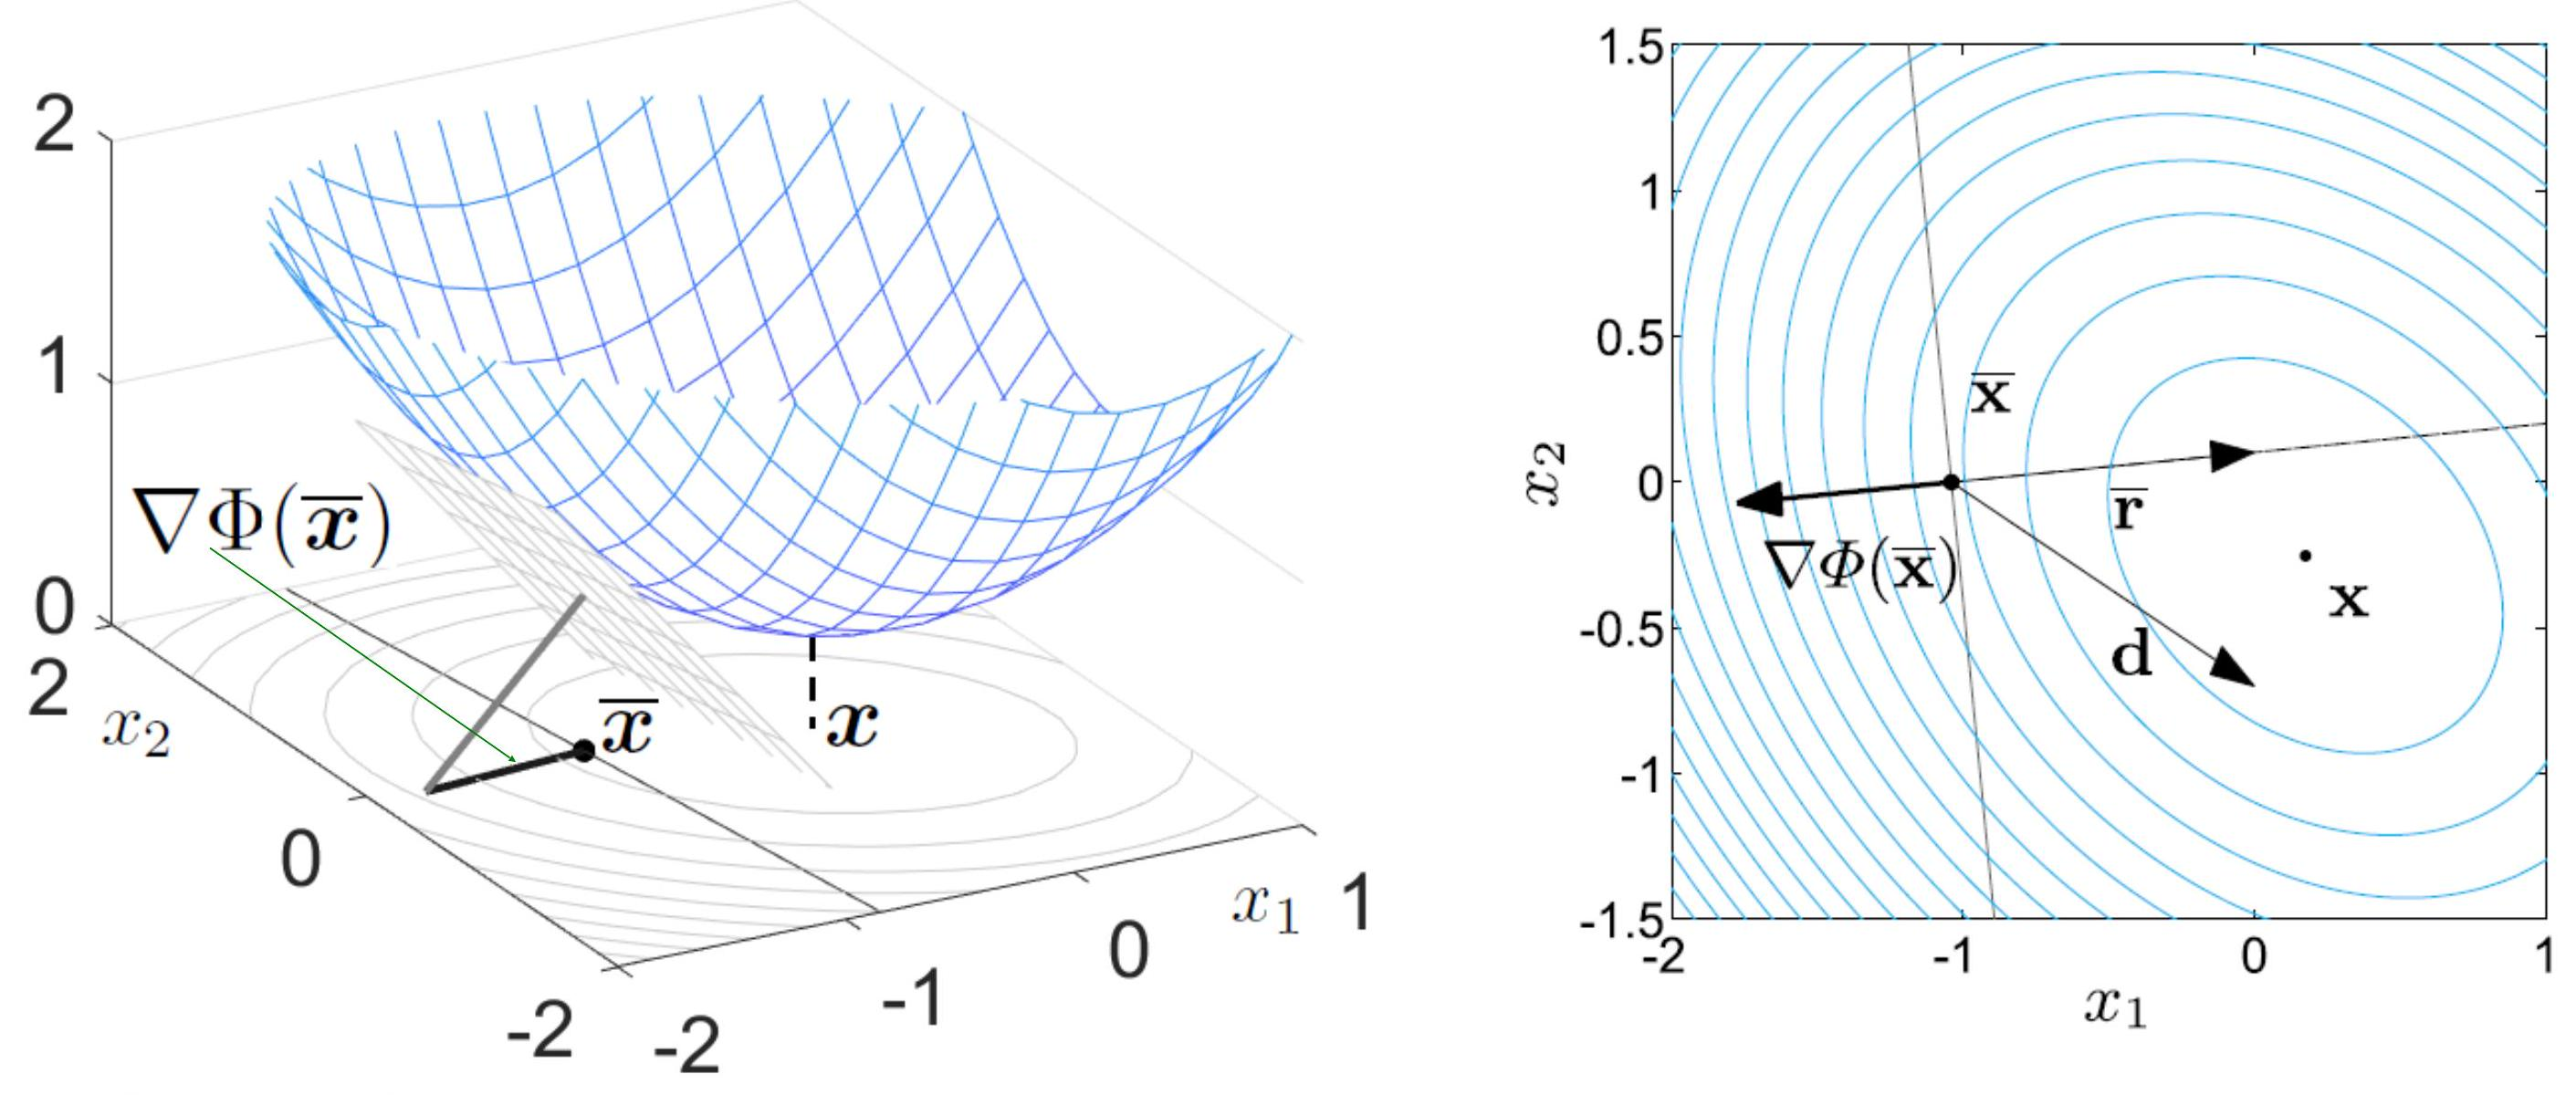
\includegraphics[scale = 0.12,center]{2023_09_05_b72ccc85584d9dc6fb5cg-077} \\ \\
Thus, if we want to minimize $\Phi(\cdot)$, we might think of taking a guess at $\mathbf{x}^{(k)}$, evaluating the gradient $\nabla \Phi\left(\mathbf{x}^{(k)}\right)$, and taking a step in the opposite direction, i.e.,
$$
\mathbf{x}^{(k+1)}=\mathbf{x}^{(k)}-\alpha_{k} \nabla \Phi\left(\mathbf{x}^{(k)}\right)
$$
Also other linear iterative methods (Jacobi, Gauss-Seidel, SOR, Richardson) use the residual as a direction for improving the solution:
\begin{itemize}
  \item Richardson: $\mathbf{x}^{(k+1)}=\mathbf{x}^{(k)}+\alpha \mathbf{r}^{(k)}$.\\
  \item Jacobi: $\mathbf{x}^{(k+1)}=\mathbf{x}^{(k)}+D^{-1} \mathbf{r}^{(k)}$.\\
  \item Gauss-Seidel: $\mathbf{x}^{(k+1)}=\mathbf{x}^{(k)}+(D-E)^{-1} \mathbf{r}^{(k)}$.\\
  \item SOR: $\mathbf{x}^{(k+1)}=\mathbf{x}^{(k)}+\omega D^{-1} \mathbf{r}^{(k)}$.\\
\end{itemize}
Steepest descendent: $\mathbf{x}^{(k+1)}=\mathbf{x}^{(k)}+\alpha_{k} \mathbf{r}^{(k)}$\\How do we choose $\alpha_{k}$, at each $k$? Remember that $\nabla \Phi(\mathbf{y})=A \mathbf{y}-\mathbf{b}=-\mathbf{r}$, we obtain:
$$
-\nabla \Phi\left(\mathbf{x}^{(k)}\right)=\mathbf{b}-A \mathbf{x}^{(k)}=\mathbf{r}^{(k)}
$$
Therefore the gradient method can be interpreted as a Richardson method with dynamic parameter $\alpha_{k}$.\\
What's the advantage?\\
That the parameter $\alpha_{k}$ can be chosen in an optimal way at each iteration $k$, that the above algorithm does no longer requires knowing the eigenvalues of $A$ (which often need to be approximated numerically) The optimal parameter $\alpha_{k}$ is chosen in order to minimize the energy by moving in the direction of the gradient. This is equivalent to asking that:
$$\frac{\mathrm{d} \Phi\left(\mathbf{x}^{(k+1)}\right)}{\mathrm{d} \alpha_k}=0$$
We have:
$$
\begin{aligned}
\Phi\left(\boldsymbol{x}^{(k+1)}\right)= & \frac{1}{2}\left(\boldsymbol{x}^{(k)}+\alpha_{k} \boldsymbol{r}^{(k)}\right)^{T} A\left(\boldsymbol{x}^{(k)}+\alpha_{k} \boldsymbol{r}^{(k)}\right)-\left(\boldsymbol{x}^{(k)}+\alpha_{k} \boldsymbol{r}^{(k)}\right)^{T} \boldsymbol{b} \\
= & \frac{1}{2}\left(\boldsymbol{x}^{(k)}\right)^{T} A \boldsymbol{x}^{(k)}+\frac{1}{2} \alpha_{k}\left(\boldsymbol{x}^{(k)}\right)^{T} A \boldsymbol{r}^{(k)}+\frac{1}{2} \alpha_{k}\left(\boldsymbol{r}^{(k)}\right)^{T} A \boldsymbol{x}^{(k)}+\frac{1}{2} \alpha_{k}^{2}\left(\boldsymbol{r}^{(k)}\right)^{T} A \boldsymbol{r}^{(k)} \\
& -\left(\boldsymbol{x}^{(k)}\right)^{T} \boldsymbol{b}-\alpha_{k}\left(\boldsymbol{r}^{(k)}\right)^{T} \boldsymbol{b} = \star
\end{aligned}
$$
Since $A=A^{T}$ we can write the following equation:
$$
\left(\boldsymbol{x}^{(k)}\right)^{T} A \boldsymbol{r}^{(k)}=\left(\boldsymbol{x}^{(k)}\right)^{T} A^{T} \boldsymbol{r}^{(k)}=\left(A \boldsymbol{x}^{(k)}\right)^{T} \boldsymbol{r}^{(k)}=\left(\boldsymbol{r}^{(k)}\right)^{T} A \boldsymbol{x}^{(k)}$$
Therefore,
$$
\begin{aligned}
0=\frac{d \Phi\left(\boldsymbol{x}^{(k+1)}\right)}{d \alpha_{k}} & =\left(\boldsymbol{r}^{(k)}\right)^{T} A \boldsymbol{x}^{(k)}+\alpha_{k}\left(\boldsymbol{r}^{(k)}\right)^{T} A \boldsymbol{r}^{(k)}-\left(\boldsymbol{r}^{(k)}\right)^{T} \boldsymbol{b} \\
& =-\left(\boldsymbol{r}^{(k)}\right)^{T} \boldsymbol{r}^{(k)}+\alpha_{k}\left(\boldsymbol{r}^{(k)}\right)^{T} A \boldsymbol{r}^{(k)}
\end{aligned}
$$
and we obtain:
$$
\alpha_{k}=\frac{\left(\boldsymbol{r}^{(k)}\right)^{T} \boldsymbol{r}^{(k)}}{\left(\boldsymbol{r}^{(k)}\right)^{T} A \boldsymbol{r}^{(k)}}
$$
We observe that:
$$
\mathbf{r}^{(k+1)}=\mathbf{b}-A \mathbf{x}^{(k+1)}=\mathbf{b}-A\left(\mathbf{x}^{(k)}+\alpha_{k} \mathbf{r}^{(k)}\right)=\mathbf{r}^{(k)}-\alpha_{k} A \mathbf{r}^{(k)}
$$
The vector-matrix product $A \mathbf{r}^{(k)}$ in the calculation of $\alpha_{k}$ is then also employed in the update of the residual $\mathbf{r}^{(k+1)}$. Computing $\mathbf{r}^{(k+1)}$ costs the sum of two vectors.

\subsection*{Pseudo-algorithm}
Given $\mathbf{x}^{(0)}$, Compute $\mathbf{r}^{(0)}=\mathbf{b}-A \mathbf{x}^{(0)}$

While (STOPPING CRITERIA)

$$
\begin{array}{ll}
\alpha_{k}=\frac{\left(\boldsymbol{r}^{(k)}\right)^{T} \boldsymbol{r}^{(k)}}{\left(\boldsymbol{r}^{(k)}\right)^{T} A \boldsymbol{r}^{(k)}} & \sim n \text { FLOPS if } A \text { is sparse } \\
\boldsymbol{x}^{(k+1)}=\boldsymbol{x}^{(k)}+\alpha_{k} \boldsymbol{r}^{(k)} & \sim n \text { FLOPS } \\
\boldsymbol{r}^{(k+1)}=\left(I-\alpha_{k} A\right) \boldsymbol{r}^{(k)} & \sim n \text { FLOPS }
\end{array}
$$
The convergence rate of the gradient method is the same as that of stationary Richardson's method with optimal parameter:
$$
\left\|\boldsymbol{e}^{(k+1)}\right\|_{A} \leq \frac{K(A)-1}{K(A)+1}\left\|\boldsymbol{e}^{(k)}\right\|_{A} \Longrightarrow\left\|\boldsymbol{e}^{(k)}\right\|_{A} \leq\left(\frac{K(A)-1}{K(A)+1}\right)^{k}\left\|\boldsymbol{e}^{(0)}\right\|_{A}
$$
\section*{The Conjugate Gradient method}
In the gradient method, two consecutive directions (the residuals) are orthogonal by construction. Indeed,
$$
0=\left(\nabla \Phi\left(\mathbf{x}^{(k)}\right), \mathbf{r}^{(k)}\right)=-\left(\mathbf{r}^{(k+1)}, \mathbf{r}^{(k)}\right)
$$
Two consecutive steepest descent directions are therefore optimal, but this is no longer true in general, i.e., the convergence behaviour of the method of steepest descent is in general poor.\\
To overcome this limit, we introduce a new updating direction, $\mathbf{d}^{(k+1)}$, in such a way that it is A-conjugate to all the previous directions $\mathbf{d}^{(j)}, j \leq k$ (i.e., orthogonal with respect to the scalar product induced by A).\\ \\
\textbf{Theorem}: In exact arithmetic the GC method converges to the exact solution in at most $n$ iterations. At each iteration $k$, the error $\mathbf{e}^{(k)}=\mathbf{x}-\mathbf{x}^{(k)}$ can be bounded by
$$
\left\|\boldsymbol{e}^{(k)}\right\|_{A} \leq \frac{2 c^{k}}{1+c^{2 k}}\left\|\boldsymbol{e}^{(0)}\right\|_{A} \text { with } c=\frac{\sqrt{K(A)}-1}{\sqrt{K(A)}+1}
$$
Round-off errors can affect the performance. \\ \\
Gradient method error bound:
$$
\left\|\boldsymbol{e}^{(k)}\right\|_{A} \leq\left(\frac{K(A)-1}{K(A)+1}\right)^{k}\left\|\boldsymbol{e}^{(0)}\right\|_{A}
$$
CG method error bound:
$$
\left\|\boldsymbol{e}^{(k)}\right\|_{A} \leq \frac{2 c^{k}}{1+c^{2 k}}\left\|\boldsymbol{e}^{(0)}\right\|_{A}
$$
\subsection*{CG Pseudo Algorithm}
Given $\mathbf{x}^{(0)}$, Compute $\mathbf{r}^{(0)}=\mathbf{b}-A \mathbf{x}^{(0)}$, set $\mathbf{d}^{(0)}=\mathbf{r}^{(0)}$ \\ 
While (STOPPING CRITERIA)
$$
\begin{aligned}
& \alpha_{k}=\frac{\left(\mathbf{d}^{(k)}\right)^{T} \mathbf{r}^{(k)}}{\left(\mathbf{d}^{(k)}\right)^{T} \mathbf{A} \mathbf{d}^{(k)}}, \\
& \mathbf{x}^{(k+1)}=\mathbf{x}^{(k)}+\alpha_{k} \mathbf{d}^{(k)}, \\
& \mathbf{r}^{(k+1)}=\mathbf{r}^{(k)}-\alpha_{k} \mathrm{~A} \mathbf{d}^{(k)}, \\
& \beta_{k}=\frac{\left(\mathrm{A} \mathbf{d}^{(k)}\right)^{T} \mathbf{r}^{(k+1)}}{\left(\mathrm{A} \mathbf{d}^{(k)}\right)^{T} \mathbf{d}^{(k)}} \\
& \mathbf{d}^{(k+1)}=\mathbf{r}^{(k+1)}-\beta_{k} \mathbf{d}^{(k)}
\end{aligned}
$$
Each iteration has a cost comparable with that of Richardson and Gradient methods.\\
Both methods converge slowly for linear system of equations with poorly conditioned matrices.
\subsection*{Preconditioned Conjugate Gradient}
A preconditioner with the same requirements discussed previously is introduced, in order to accelerate convergence.
Let $\mathrm{A}$ and $\mathrm{P}$ be SDP. We consider the following preconditioned system
$$
\widehat{A} \widehat{\boldsymbol{x}}=\widehat{\boldsymbol{b}}
$$
where:
$$\underbrace{P^{-1}AP^{-T}}_{\widehat{A}} \underbrace{P^T\boldsymbol{x}}_{\widehat{\boldsymbol{x}}}=\underbrace{P^{-1}\boldsymbol{b}}_{\widehat{\boldsymbol{b}}}$$
Given $\mathbf{x}^{(0)}$, Compute $\mathbf{r}^{(0)}=\mathbf{b}-A \mathbf{x}^{(0)}$, set $\mathbf{d}^{(0)}=\mathbf{r}^{(0)}$\\
While (STOPPING CRITERIA)
$$
\begin{aligned}
& \alpha_{k}=\frac{\mathbf{z}^{(k)^{T}} \mathbf{r}^{(k)}}{\left(\operatorname{A}\mathbf{d}^{(k)}\right)^{T} \mathbf{d}^{(k)}}, \\
& \mathbf{x}^{(k+1)}=\mathbf{x}^{(k)}+\alpha_{k} \mathbf{d}^{(k)}, \\
& \mathbf{r}^{(k+1)}=\mathbf{r}^{(k)}-\alpha_{k} \mathrm{A}\mathbf{d}^{(k)}, \\
& \mathrm{P} \mathbf{z}^{(k+1)}=\mathbf{r}^{(k+1)},
\end{aligned}
$$
$$
\beta_{k}=\frac{\left(\operatorname{Ad}^{(k)}\right)^T \mathbf{z}^{(k+1)}}{\left(\mathbf{A d}^{(k)}\right)^T \mathbf{d}^{(k)}}
$$
$$
\mathbf{d}^{(k+1)}=\mathbf{z}^{(k+1)}-\beta_{k} \mathbf{d}^{(k)}
$$

\subsection*{The PCG method, error bounds}
$$
\left\|\boldsymbol{e}^{(k)}\right\|_{A} \leq \frac{2 c^{k}}{1+c^{2 k}}\left\|\boldsymbol{e}^{(0)}\right\|_{A} \quad \text { with } \quad c=\frac{\sqrt{K\left(P^{-1} A\right)}-1}{\sqrt{K\left(P^{-1} A\right)}+1}
$$
If the preconditioner is a "good" preconditioner then
$$
\frac{\sqrt{K\left(P^{-1} A\right)}-1}{\sqrt{K\left(P^{-1} A\right)}+1}<\frac{\sqrt{K(A)}-1}{\sqrt{K(A)}+1}
$$
\section*{Krylov-space methods}

The iterative methods that are today applied for solving large-scale linear systems are mostly preconditioned Krylov (sub)space solvers.\\ \\
For linear iterative methods (with $P=I, \alpha_{k}=1$ ) as those we have seen before, we have:
$$
\mathbf{x}^{(k+1)}=\mathbf{x}^{(k)}+\mathbf{r}^{(k)} \quad k \geq 1
$$
The following recursive relation for the residuals holds
$$
\mathbf{r}^{(k+1)}=\mathbf{r}^{(k)}-A \mathbf{r}^{(k)} \quad k \geq 1
$$
From the above identity, it follows by induction, that
$$
\mathbf{r}^{(k)}=p_{k-1}(A) \mathbf{r}^{(0)} \in \operatorname{span}\left\{\mathbf{r}^{(0)}, A \mathbf{r}^{(0)}, \ldots, A^{k-1} \mathbf{r}^{(0)}\right\}
$$
where $p_{r}(z)=(1-z)^{r}$ is a polynomial of exact degree $r$.
From the previous relations, we have that:
$$
\mathbf{x}^{(k)}=\mathbf{x}^{(0)}+\mathbf{r}^{(0)}+\ldots+\mathbf{r}^{(k-1)}=\mathbf{x}^{(0)}+q_{k-1}(A) \mathbf{r}^{(0)}
$$
with a polynomial $q_{n-1}$ of exact degree $n-1$.
So $\mathbf{x}^{(k)}$ lies in the affine space.
$$
\mathbf{x}^{(0)}+\operatorname{span}\left\{\mathbf{r}^{(0)}, A \mathbf{r}^{(0)}, \ldots, A^{k-1} \mathbf{r}^{(0)}\right\}
$$
obtained by shifting the subspace of $\mathbf{r}^{k-1}$.\\ \\ 
\textbf{Definition of Krylov (sub)space}. Given a nonsingular $A \in \mathbb{R}^{n \times n}$ and $\mathbf{y} \in \mathbb{R}^{n}, \mathbf{y} \neq \mathbf{0}$, the $k^{th}$ Krylov (sub)space $\mathscr{K}_{k}(A, \mathbf{y})$ generated by $A$ from $\mathbf{y}$ is:
$$
\mathscr{K}_{k}(A, \mathbf{y}):=\operatorname{span}\left(\mathbf{y}, A \mathbf{y}, \ldots, A^{k-1} \mathbf{y}\right)
$$
Clearly, it holds that:
$$\mathscr{K}_{1}(A, \mathbf{y}) \subseteq \mathscr{K}_{2}(A, \mathbf{y}) \subseteq \ldots$$
Can we expect to find the exact solution $\mathbf{x}$ of $A \mathbf{x}=\mathbf{b}$ in one of those affine space?\\ \\
\textbf{Lemma.} Let $\mathbf{x}$ be the solution of $A \mathbf{x}=\mathbf{b}$ and let $\mathbf{x}^{(0)}$ be any initial approximation of it and $\mathbf{r}^{(0)}=\mathbf{b}-A \mathbf{x}^{(0)}$ the corresponding residual. Moreover, let $\nu=\nu\left(\mathbf{r}^{(0)}, A\right)$ be the so called grade of $\mathbf{r}^{(0)}$ with respect to $A$. Then:
$$
\mathbf{x} \in \mathbf{x}^{(0)}+\mathscr{K}_{\nu}\left(A, \mathbf{r}^{(0)}\right)
$$

\subsection*{Grade of $\mathbf{y}$ with respect to $A$}
\textbf{Lemma.} There is a positive integer $\nu=\nu(\mathbf{y}, A)$, called grade of $\mathbf{y}$ with respect to $\mathrm{A}$, such that:
$$
\operatorname{dim}\left(\mathscr{K}_{s}(A, y)\right)=\left\{\begin{array}{l}
s \text { if } s < \nu \\
\nu \text { if } s \geq \nu
\end{array}\right.
$$
$\mathscr{K}_{\nu}(A, \mathbf{y})$ is is the smallest $\mathrm{A}$-invariant subspace that contains $\mathbf{y}$.\\ \\
\textbf{Lemma.} The nonnegative integer $\nu=\nu(\mathbf{y}, A)$ of $\mathbf{y}$ with respect to $A$ satisfies:
$$
\nu(\mathbf{y}, A)=\min \left\{s \mid A^{-1} \mathbf{y} \in \mathscr{K}_{s}(A, y)\right\}
$$
The idea behind Krylov space solvers is to generate a sequence of approximate solutions $\mathbf{x}^{(k)} \in \mathbf{x}^{(0)}+\mathscr{K}_{k}\left(A, \mathbf{r}^{(0)}\right)$ of $A \mathbf{x}=\mathbf{b}$ so that the corresponding residuals $\mathbf{r}^{(k)} \in \mathscr{K}_{k+1}\left(A, \mathbf{r}^{(0)}\right)$ "converge" to the zero vector $\mathbf{0}$.\\ \\
Here, "converge" may also mean that after a finite number of steps, $\mathbf{r}^{(k)}=\mathbf{0}$, so that $\mathbf{x}^{k}=\mathbf{x}$ and the process stops. This is in particular true (in exact arithmetic) if a method ensures that the residuals are linearly independent: then $\mathbf{r}^{(\nu)}=\mathbf{0}$. In this case we say that the method has the finite termination property.\\ \\
\textbf{Definition:} A (standard) Krylov space method for solving a linear system $A \mathbf{x}=\mathbf{b}$ or, briefly, a Krylov space solver is an iterative method starting from some initial approximation $\mathbf{x}^{(0)}$ and the corresponding residual $\mathbf{r}^{(0)}$ until it possibly finds the exact solution, iterating $\mathbf{x}^{(\mathbf{k})}$ such that:
$$
\mathbf{x}^{(k)}=\mathbf{x}^{(0)}+p_{k-1}(A) \mathbf{r}^{(0)}
$$
with a polynomial $p_{k-1}(A)$ of exact degree $k-1$. For some $k, \mathbf{x}^{(k)}$ may not exist or $p_{k-1}(A)$ may have lower degree.\\ \\
In some widely used Krylov space solvers (e.g., BICG) there may exist exceptional situations, where for some $n$ the iterate $\mathbf{x}_n$ and the residual $\mathbf{r}_n$ are not defined. In other Krylov space solvers (e.g., CR), there may be indices where $\mathbf{x}_n$ exists, but the polynomial $q_{n-1}$ is of lower degree than $n-1$.
\subsection*{Krylov space methods}
When applied to large real-world problems Krylov space solvers often converge very slowly - if at all. In practice, Krylov space solvers are therefore nearly always applied with preconditioning:
$$
A \mathbf{x}=\mathbf{b} \quad \Longleftrightarrow \quad \underbrace{P^{-1}_L A P_R}_{\hat{A}} \underbrace{P^{-1}_R\mathbf{x}}_{\hat{\mathbf{x}}}=\underbrace{P^{-1} \mathbf{b}}_{\hat{\mathbf{b}}} \quad \Longleftrightarrow \quad \hat{A} \hat{\mathbf{x}}=\hat{\mathbf{b}}, \quad P_R \hat{\mathbf{x}}=\mathbf{x}
$$
Applying a preconditioned Krylov space solver just means to apply the method to $\hat{A} \hat{\mathbf{x}}=\hat{\mathbf{b}}$.
\section*{The CG method is a Krylov space solver}
CG is the archetype of a Krylov space solver that is an orthogonal projection method. By definition, such a method chooses the step length $\alpha_{k}$ so that $\mathbf{x}^{(k+1)}$ is locally optimal on the search line.
$$
\begin{aligned}
& \alpha_{k}=\frac{\left(\mathbf{d}^{(k)}\right)^{T} \mathbf{r}^{(k)}}{\left(\mathbf{d}^{(k)}\right)^{T} \mathrm{~A} \mathbf{d}^{(k)}}, \\
& \mathbf{x}^{(k+1)}=\mathbf{x}^{(k)}+\alpha_{k} \mathbf{d}^{(k)}, \\
& \mathbf{r}^{(k+1)}=\mathbf{r}^{(k)}-\alpha_{k} \mathrm{~A} \mathbf{d}^{(k)}, \\
& \beta_{k}=\frac{\left(\mathrm{A} \mathbf{d}^{(k)}\right)^{T} \mathbf{r}^{(k+1)}}{\left(\mathrm{A}\mathbf{d}^{(k)}\right)^{T} \mathbf{d}^{(k)}} \\
& \mathbf{d}^{(k+1)}=\mathbf{r}^{(k+1)}-\beta_{k} \mathbf{d}^{(k)}
\end{aligned}
$$
But does it also yield the best $
\mathbf{x}^{(k+1)} \in \mathbf{x}^{(0)}+\operatorname{span}\left\{\mathbf{d}_{0}, \mathbf{d}_{1}, \ldots, \mathbf{d}_{k}\right\} ?
$\\ 
The next result shows that:
$$
\operatorname{span}\left\{\mathbf{d}_{0}, \mathbf{d}_{1}, \ldots, \mathbf{d}_{k}\right\}=\mathscr{K}_{k+1}\left(A, \mathbf{r}^{(0)}\right)
$$
\textbf{Theorem}: The Conjugate Gradient (CG) method produces approximate solutions, $\mathbf{x}^{(k)}$, that belong to the affine space $\mathbf{x}^{(0)}+\mathscr{K}_{k}\left(A, \mathbf{r}^{(0)}\right)$.\\ \\
\textbf{Theorem.} The CG method yields approximate solutions $\mathbf{x}_n \in \mathbf{x}_0+\mathcal{K}_n\left(\mathbf{A}, \mathbf{r}_0\right)$ that are optimal in the sense that they minimize the energy norm (A-norm) of the error (i.e., the $\mathbf{A}^{-1}$-norm of the residual) for $\mathbf{x}_n$ from this affine space.\\ \\ 
The residual can be updated using the following formula:
$$
\mathbf{r}^{(k+1)}=\mathbf{r}^{(k)}-\alpha_{k} \mathrm{A}\mathbf{d}^{(k)},
$$
The value of $\beta_{k}$ can be calculated using this formula:
$$
\beta_{k}=\frac{\left(\operatorname{A}\mathbf{d}^{(k)}\right)^{T} \mathbf{r}^{(k+1)}}{\left(\operatorname{A}\mathbf{d}\right)^{(k)T} \mathbf{d}^{(k)}}
$$

$$
\mathbf{d}^{(k+1)}=\mathbf{r}^{(k+1)}-\beta_{k} \mathbf{d}^{(k)}
$$ 
\section*{Krylov space solvers for nonsymmetric systems}
Solving nonsymmetric linear systems iteratively with Krylov space solvers is considerably more difficult and costly than symmetric systems. There are two different ways to generalize CG:
\begin{itemize}
  \item Maintain the orthogonality of the projection and the related minimality of the error by constructing either orthogonal residuals $\mathbf{x}^{(k)}$ (generalized CG - GCG). Then, the recursions involve all previously constructed residuals or search directions and all previously constructed iterates.\\
  \item Maintain short recurrence formulas for residuals, direction vectors and iterates (biconjugate gradient (BiCG) method, Lanczos-type product methods (LTPM)). The resulting methods are at best oblique projection methods. There is no minimality property of error or residuals vectors.\\
\end{itemize}

\section*{The Biconjugate gradient (BiCG) method}
While CG (for spd A) has mutually orthogonal residuals $\mathbf{r}^{(k)}$ with $\mathbf{r}^{(k)}=p_{k}(A) \mathbf{r}^{(0)} \in \operatorname{span}\left\{\mathbf{r}^{(0)}, A \mathbf{r}^{(0)}, \ldots, A^{k} \mathbf{r}^{(0)}\right\}=\mathscr{K}_{k+1}\left(A, \mathbf{r}^{(0)}\right)$, BiCG constructs in the same spaces residuals that are orthogonal to a dual Krylov space spanned by "shadow residuals".
$$\mathbf{r}_n=p_n(\mathbf{A}) \mathbf{r}_0 \in \operatorname{span}\left\{\mathbf{r}_0, \mathbf{A r}_0, \ldots, \mathbf{A}^n \mathbf{r}_0\right\}=: \mathcal{K}_{n+1}\left(\mathbf{A}, \mathbf{r}_0\right)$$
$$
\tilde{\mathbf{r}}^{(k)}=p_{k}\left(A^{T}\right) \tilde{\mathbf{r}}^{(0)} \in \operatorname{span}\left\{\tilde{\mathbf{r}}^{(0)}, A^{T} \tilde{\mathbf{r}}^{(0)}, \ldots,\left(A^{T}\right)^{k} \tilde{\mathbf{r}}^{(0)}\right\}=\mathscr{K}_{k+1}\left(A^{T}, \tilde{\mathbf{r}}^{(0)}\right) =: \tilde{\mathscr{K}}_{k+1}
$$
The initial shadow residual $\tilde{\mathbf{r}}^{(0)}$ can be chosen freely. So, BiCG requires two matrix-vector multiplications to extend $\mathscr{K}_{k}$ and $\tilde{\mathscr{K}}_{k}$ : one multiplication by $A$ and one by $A^{T}$. 
The use of the transpose of A allows us to construct a dual Krylov space that is different from the original Krylov space. This is crucial for handling non-symmetric matrices, as it allows us to construct residuals that are orthogonal to a different space.
However, this comes at a cost: while the CG method requires one matrix-vector multiplication per iteration (by $A$), the BiCG method requires two $\bigl( $one by $A$ and one by $A^T \bigl)$. This makes the BiCG method more computationally expensive than the CG method.
\subsection*{The BiCGSTAB method}
The biconjugate gradient stabilized method (BiCGSTAB), is a variant of the biconjugate gradient method (BiCG) and has faster and smoother convergence than the original BiCG.\\
It is unnecessary to explicitly keep track of the residuals and search directions of BiCG. In other words, the BiCG iterations can be performed implicitly. \\ \\
In other words, BiCGSTAB simplifies the process by reducing the amount of data that needs to be stored and manipulated, leading to potentially significant savings in computational resources. This makes it a more efficient method for solving nonsymmetric linear systems. \\ \\

Choose $\mathbf{x}^{(0)}, \hat{\mathbf{x}}^{(0)}, \hat{\mathbf{b}}$,

Compute $\mathbf{r}^{(0)}=\mathbf{b}-A \mathbf{x}^{(0)}$,

Compute $\hat{\mathbf{r}}^{(0)}=\mathbf{b}-\hat{\mathbf{x}}^{(0)} A$

$\mathbf{d}_{0}=\mathbf{r}^{(0)}, \hat{\mathbf{d}}_{0}=\hat{\mathbf{r}}^{(0)}$

WHILE(STOPPING CRITERIA)

$\alpha_{k}=\frac{\hat{\mathbf{r}}^{(k)} \mathbf{r}^{(k)}}{\hat{\mathbf{d}}_{k} A \mathbf{d} k}$

$\mathbf{x}^{(k+1)}=\mathbf{x}^{(k)}+\alpha_{k} \mathbf{d}_{k}$

$\hat{\mathbf{x}}^{(k+1)}=\hat{\mathbf{x}}^{(k)}+\alpha_{k} \hat{\mathbf{d}}_{k}$

$\mathbf{r}^{(k+1)}=\mathbf{r}^{(k)}-\alpha_{k} A \mathbf{r}^{(k)} $

$\hat{\mathbf{r}}^{(k+1)}=\hat{\mathbf{r}}^{(k)}-\alpha_{k} A \hat{\mathbf{r}}^{(k)}$ 

$ \beta_{k}= \hat{\mathbf{r}}^{(k)} \mathbf{r}^{(k)} $

$ \hat{\mathbf{r}}^{(k)} \mathbf{r}^{(k)} $

$ \mathbf{d}_{k+1}=\mathbf{r}^{(k+1)}+\beta_{k} \mathbf{d}_{k} $

$ \hat{\mathbf{d}}_{k+1}=\hat{\mathbf{r}}^{(k+1)}+\beta_{k} \hat{\mathbf{d}}_{k} $



\section*{The GMRES method}
The goal of GMRES is to find a vector within this Krylov subspace that minimizes the residual, or the difference between the actual solution and the approximated solution. This is done using the Arnoldi iteration, which is a process that constructs an orthogonal basis for the Krylov subspace.\\ \\
Recall that the $k$-th Krilov space $\mathscr{K}_{k}=\mathscr{K}_{k}\left(A, \mathbf{r}^{(0)}\right)$ is given by:
$$\mathscr{K}_{k}\left(A, \mathbf{r}^{(0)}\right)=\operatorname{span}\left\{\mathbf{r}^{(0)}, A \mathbf{r}^{(0)}, \ldots, A^{k-1} \mathbf{r}^{(0)}\right\}.$$
GMRES approximates the exact solution of $A \mathbf{x}=\mathbf{b}$ by the vector $\mathscr{K}_{k}\left(A, \mathbf{r}^{(0)}\right)$ that minimizes the Euclidean norm of the residual $\mathbf{r}^{(k)}=b-A \mathbf{x}^{(k)}$. \\
The Arnoldi iteration is a method used to find an orthonormal basis for the Krylov subspace. The Krylov subspace is spanned by the vectors $\mathbf{r}^{(0)}, A \mathbf{r}^{(0)}, \ldots, A^{k-1} \mathbf{r}^{(0)}$. However, these vectors can be close to linearly dependent (i.e., one vector can be approximated as a linear combination of the others), which can cause numerical instability.\\ 
To avoid this issue, the Arnoldi iteration constructs a set of orthonormal vectors $\mathbf{q}_{1}, \mathbf{q}_{2}, \ldots, \mathbf{q}_{k}$ that span the same space as the original vectors. These orthonormal vectors form a stable basis for the Krylov subspace, which is crucial for the stability and accuracy of the GMRES method.\\ \\
Choose $\mathbf{x}^{(0)}$, Compute $\mathbf{r}^{(0)}=\mathbf{b}-A \mathbf{x}^{(0)}$,

Set $\mathbf{q}_{1}=\mathbf{r}^{(0)} /\left\|\mathbf{r}^{(0)}\right\|_{2}$

WHILE(STOPPING CRITERIA)

Compute $\mathbf{q}_{k}$ with the Arnoldi method

Form $\mathbf{Q}_{k}$ as the $n \times k$ matrix formed by $\mathbf{q}_{1}, \mathbf{q}_{2}, \ldots, \mathbf{q}_{k}$

Find $\mathbf{y}^{(k)}$ which minimize $\left\|\mathbf{r}^{(k)}\right\|_{2}$

Compute $\mathbf{x}^{(k+1)}=\mathbf{x}^{(0)}+Q_{k} \mathbf{y}^{(k)}$

end

\subsection*{GMRES some remarks}
Remarks:
\begin{itemize}
  \item At every iteration $k$, a matrix-vector product must be computed, which costs about $n^{2}$ FLOPS for dense matrices. If $A$ is sparse, this cost is $O(n)$ FLOPS.

  \item In addition to the matrix-vector product, $O(k n)$ FLOPS operations must be computed at the $k$-th iteration.

  \item The $k$-th iterate minimises the residual in the Krylov subspace $\mathscr{K}_{k}\left(A, \mathbf{r}^{(0)}\right)$. In exact arithmetic, since every subspace is (strictly) contained in the next subspace, the residual does not increase. Therefore, after $n=\operatorname{size}(A)$ iterations, the Krylov space $\mathscr{K}_{n}\left(A, \mathbf{r}^{(0)}\right)$ is the whole of $\mathbb{R}^{n}$. hence the GMRES method has finite termination property in exact arithmetic, but this does not happen in practice.

\end{itemize}

\subsection*{GMRES convergence, special cases}
\begin{itemize}
  \item If $A_{S}=\left(A+A^{T}\right) / 2$ is SPD, then
\end{itemize}
$$
\left\|\mathbf{r}^{(k)}\right\| \leq\left[1-\frac{\lambda_{\min }^{2}\left(A_{S}\right)}{\lambda_{\max }\left(A^{T} A\right)}\right]^{k / 2}\left\|\mathbf{r}^{(0)}\right\|.
$$
\begin{itemize}
  \item If $A$ is $S P D$, then
\end{itemize}
$$
\left\|\mathbf{r}^{(k)}\right\| \leq\left[\frac{\left[K_{2}(A)\right]^{2}-1}{\left[K_{2}(A)\right]^{2}}\right]^{k / 2}\left\|\mathbf{r}^{(0)}\right\|.
$$


\chapter{Elements of Multigrid}
This chapter follows closely the first three chapters of the following book: "A Multigrid Tutorial: Second Edition", by  William L. Briggs, Van Emden Henson, Steve F. McCormick. It is recommended to read them to gain a deeper understanding.
\\ \\
It is possible to expand arbitrary vectors in terms of a set of eigenvectors of the  matrix, if it has full rank, as it happens in many physical problems.
Let $\textbf{e}^{(0)}$ be the error in an initial guess used in a iterative method. Then
it is possible to represent $\textbf{e}^{(0)}$
 using the eigenvectors of $R$ in the form:
 $$\textbf{e}^{(0)} = \sum_{k=1}^{n} c_k \textbf{w}_{k},$$
 where the coefficients $c_k \in \mathbb{R}$  give the "amount" of each mode in the error.
 Many standard iterative methods, like Jacobi or Gauss Seidel, possess the smoothing property, which makes these methods very effective at eliminating the high-frequency or oscillatory components of the error, while leaving the low-frequency or smooth components relatively unchanged. The immediate issue is whether these methods can be modified in some way to make them effective on all error components.\\ \\
One way to improve a relaxation scheme, at least in its early stages, is to use a good initial guess. A well-known technique for obtaining an improved initial guess is to perform some preliminary iterations on a coarse grid. Relaxation on a coarse grid is less expensive because there are fewer unknowns to be updated. Moreover, as mentioned before, because the convergence factor behaves like $1-O\left(h^{2}\right)$, the coarse grid will have a marginally improved convergence rate. This line of reasoning at least suggests that coarse grids might be worth considering.\\ \\
With the coarse grid idea in mind, we can think more carefully about its implications. Recall that most basic relaxation schemes suffer in the presence of smooth components of the error. Assume that a particular relaxation scheme has been applied until only smooth error components remain.  We now ask what these smooth
components look like on a coarser grid. It is easy to understand that 
in passing from the fine grid to the coarse grid, a mode becomes more oscillatory.\\ \\
A smooth wave with $k=4$ on a grid $\Omega^{h}$ with $n=12$ points has been projected directly to the grid $\Omega^{2 h}$ with $n=6$ points. On this coarse grid, the original wave still has a wavenumber of $k=4$. We see that a smooth wave on $\Omega^{h}$ looks more oscillatory on $\Omega^{2 h}$. \\
To be more precise, note that the grid points of the coarse grid $\Omega^{2 h}$ are the even-numbered grid points of the fine grid $\Omega^{h}$. Consider the $k$-th mode on the fine grid evaluated at the even-numbered grid points. If $1 \leq k<\frac{n}{2}$, its components may be written as:\\ \\
$  w_{k, 2 j}^{h}=\sin \left(\frac{2 j k \pi}{n}\right)=\sin \left(\frac{j k \pi}{n / 2}\right)=w_{k, j}^{2 h}, \quad 1 \leq k<\frac{n}{2}$. \\ \\
Notice that superscripts have been used to indicate the grids on which the vectors are defined. From this identity, we see that the $k$-th mode on $\Omega^{h}$ becomes the $k$-th mode on $\Omega^{2 h}$. This fact is easier to understand by noting that there are half as many modes on $\Omega^{2 h}$ as there are on $\Omega^{h}$.\\ \\
The important consequence of this fact is that in passing from the fine grid to the coarse grid, a mode becomes more oscillatory. This is true provided that $1 \leq k<\frac{n}{2}$. It should be verified that the $k=\frac{n}{2}$ mode on $\Omega^{h}$ becomes the zero vector on $\Omega^{2 h}$.\\
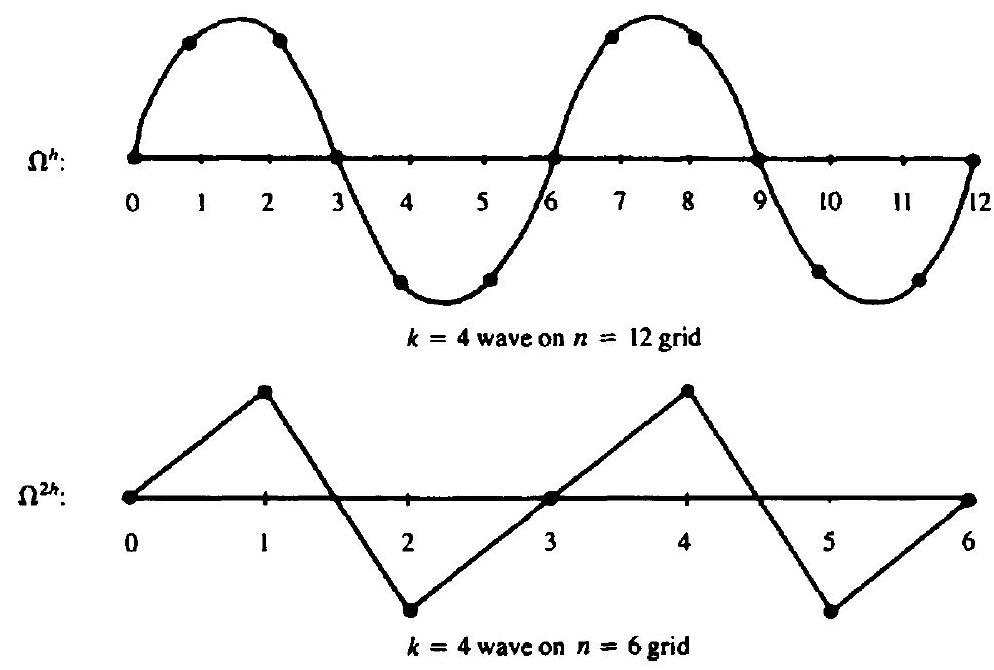
\includegraphics[max width=\textwidth, center]{2023_10_10_f3de0b9400b097aecf14g-045}\\
\textbf{Figure 3.1}: Wave with wavenumber $k=4$ on $\Omega^{h}$ ( $n=12$ points) projected onto $\Omega^{2 h}$ ( $n=6$ points). The coarse grid "sees" a wave that is more oscillatory on the coarse grid than on the fine grid. \\ \\
As an aside, it is worth mentioning that fine-grid modes with $k>\frac{n}{2}$ undergo a more curious transformation. Through the phenomenon of aliasing, the $k$-th mode on $\Omega^{h}$ becomes the $(n-k)$-th mode on $\Omega^{2 h}$ when $k>\frac{n}{2}$. In other words, the oscillatory modes of $\Omega^{h}$ are misrepresented as relatively smooth modes on $\Omega^{2 h}$. \\ \\
The important point is that smooth modes on a fine grid look less smooth on a coarse grid. This suggests that when relaxation begins to stall, signaling the predominance of smooth error modes, it is advisable to move to a coarser grid. There, the smooth error modes appear more oscillatory and relaxation will be more effective. The question is: how do we move to a coarser grid and relax on the more oscillatory error modes? \\ \\ 
 Recall that we have an equation for the error itself, namely, the residual equation. If $\mathbf{v}$ is an approximation to the exact solution $\mathbf{u}$, then the error $\mathbf{e}=\mathbf{u}-\mathbf{v}$ satisfies:
$$
A \mathbf{e}=\mathbf{r}=\mathbf{f}-A \mathbf{v}
$$
which says that we can relax directly on the error by using the residual equation. There is another argument that justifies the use of the residual equation.
Relaxation on the original equation $A \mathbf{u}=\mathbf{f}$ with an arbitrary initial guess $\mathbf{v}$ is equivalent to relaxing on the residual equation $A \mathbf{e}=\mathbf{r}$ with the specific initial guess $\mathbf{e}=\mathbf{0}$. This intimate connection between the original and the residual equations further motivates the use of the residual equation.\\ \\
Given the equation $A \mathbf{u} = \mathbf{f}$, where $A$ is the coefficient matrix, $\mathbf{u}$ is the unknown vector, and $\mathbf{f}$ is the right-hand side vector. If $\mathbf{v}$ is an approximation to $\mathbf{u}$, the error $\mathbf{e}$ can be defined as $\mathbf{e} = \mathbf{u} - \mathbf{v}$. Substituting $\mathbf{u} = \mathbf{v} + \mathbf{e}$ into the original equation and simplifying gives $A\mathbf{e} = \mathbf{f} - A\mathbf{v} = \mathbf{r}$, which is the residual equation.\\ \\
This demonstrates that relaxing directly on the error using the residual equation is equivalent to relaxing on the original equation with an arbitrary initial guess, as both the error and the residual are linked through the same linear system governed by matrix $A$"\\ \\
We must now gather these loosely connected ideas. We know that many relaxation schemes possess the smoothing property. This leads us to consider using coarser grids during the computation to focus the relaxation on the oscillatory components of the error. In addition, there seems to be good reason to involve the residual equation in the picture. We now try to give these ideas a little more definition by proposing two strategies. \\ \\
We begin by proposing a strategy that uses coarse grids to obtain better initial guesses.

\begin{itemize}
  \item Relax on $A \mathbf{u}=\mathbf{f}$ on a very coarse grid to obtain an initial guess for the next finer grid.

  \item Relax on $A \mathbf{u}=\mathbf{f}$ on $\Omega^{4 h}$ to obtain an initial guess for $\Omega^{2 h}$.

  \item Relax on $A \mathbf{u}=\mathbf{f}$ on $\Omega^{2 h}$ to obtain an initial guess for $\Omega^{h}$.

  \item Relax on $A \mathbf{u}=\mathrm{f}$ on $\Omega^{h}$ to obtain a final approximation to the solution.

\end{itemize}
This idea of using coarser grids to generate improved initial guesses is the basis of a strategy called nested iteration. Although the approach is attractive, it also leaves some questions. For instance, what does it mean to relax on $A \mathbf{u}=\mathbf{f}$ on $\Omega^{2 h}$ ? We must somehow define the original problem on the coarser grids. Also, what happens if, having once reached the fine grid, there are still smooth components in the error? We may have obtained some improvement by using the coarse grids, but the final iteration will stall if smooth components still remain. We return to these questions and find answers that will allow us to use nested iteration in a very powerful way. \\ \\
A second strategy incorporates the idea of using the residual equation to relax on the error. It can be represented by the following procedure:
\begin{itemize}
  \item Relax on $A \mathbf{u}=\mathrm{f}$ on $\Omega^{h}$ to obtain an approximation $\mathbf{v}^{h}$.

  \item Compute the residual $\mathbf{r}=\mathbf{f}-A \mathbf{v}^{h}$.

\end{itemize}
Relax on the residual equation $A \mathbf{e}=\mathbf{r}$ on $\Omega^{2 h}$ to obtain an approximation to the error $\mathrm{e}^{2 h}$.

\begin{itemize}
  \item Correct the approximation obtained on $\Omega^{h}$ with the error estimate obtained on $\Omega^{2 h}: \mathbf{v}^{h} \leftarrow \mathbf{v}^{h}+\mathbf{e}^{2 h}$.
\end{itemize}
This procedure is the basis of what is called the correction scheme. Having relaxed on the fine grid until convergence deteriorates, we relax on the residual equation on a coarser grid to obtain an approximation to the error itself. We then return to the fine grid to correct the approximation first obtained there.
There is a rationale for using this correction strategy, but it also leaves some questions to be answered. For instance, what does it mean to relax on $A \mathbf{e}=r$ on $\Omega^{2 h}$ ? To answer this question, we first need to know how to compute the residual.

\begin{center}
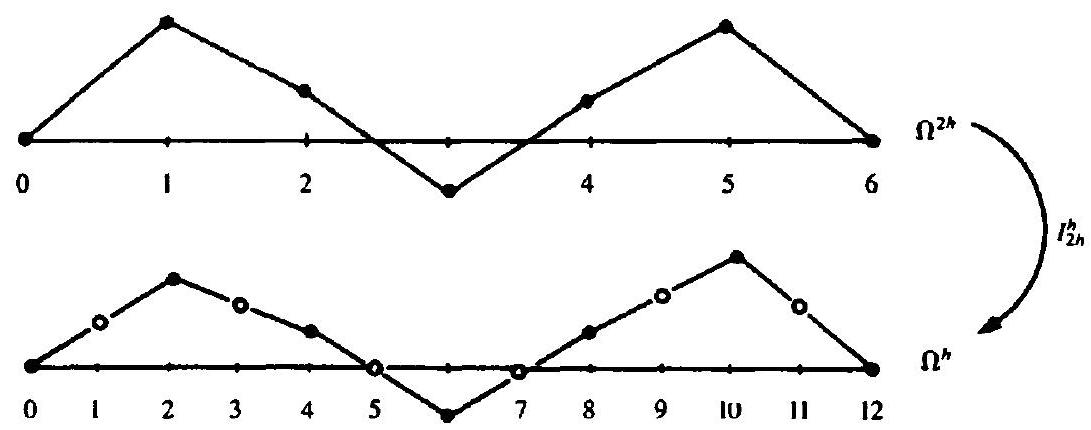
\includegraphics[max width=\textwidth]{2023_10_10_f3de0b9400b097aecf14g-047}
\end{center} 
\textbf{Figure 3.2}: Interpolation of a vector on coarse grid $\Omega^{2 h}$ to fine grid $\Omega^{h}$ on $\Omega^{h}$ and transfer it to $\Omega^{2 h}$.\\ \\
We also need to know how to relax on $\Omega^{2 h}$ and what initial guess should be used. Moreover, how do we transfer the error estimate from $\Omega^{2 h}$ back to $\Omega^{h}$? These questions suggest that we need mechanisms for transferring information between the grids. We now turn to this important consideration. \\
In our discussion of intergrid transfers, we consider only the case in which the coarse grid has twice the grid spacing of the next finest grid. This is a nearly universal practice, because there is usually no advantage in using grid spacings with ratios other than 2. Think for a moment about the step in the correction scheme that requires transferring the error approximation $\mathbf{e}^{2 h}$ from the coarse grid $\Omega^{2 h}$ to the fine grid $\Omega^{h}$. This is a common procedure in numerical analysis and is generally called interpolation or prolongation. Many interpolation methods could be used. Fortunately, for most multigrid purposes, the simplest of these is quite effective. For this reason, we consider only linear interpolation. \\ \\
The linear interpolation operator will be denoted $I_{2 h}^{h}$. It takes coarse-grid vectors and produces fine-grid vectors according to the rule $I_{2 h}^{h} \mathbf{v}^{2 h}=\mathbf{v}^{h}$, where
$$
\begin{cases}
v_{2 j}^{h} & =v_{j}^{2 h} \\
v_{2 j+1}^{h} & =\frac{1}{2}\left(v_{j}^{2 h}+v_{j+1}^{2 h}\right), \quad 0 \leq j \leq \frac{n}{2}-1
\end{cases}
$$
\textbf{Figure 3.2} shows graphically the action of $I_{2 h}^{h}$. At even-numbered fine-grid points, the values of the vector are transferred directly from $\Omega^{2 h}$ to $\Omega^{h}$. At odd-numbered fine-grid points, the value of $v^{h}$ is the average of the adjacent coarse-grid values.\\ \\
In anticipation of discussions to come, we note that $I_{2 h}^{h}$ is a linear operator from $\mathbb{R}^{\frac{n}{2}-1}$ to $\mathbb{R}^{n-1}$. It has full rank and the trivial null space, $\mathcal{N}=\{0\}$.
How well does this interpolation process work? First assume that the "real" error (which is not known exactly) is a smooth vector on the fine grid.\\ \\
a)
\begin{center}
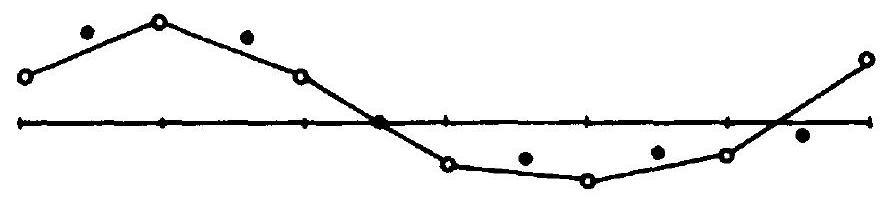
\includegraphics[max width=\textwidth]{2023_10_10_f3de0b9400b097aecf14g-048}
\end{center}
(b)
\begin{center}
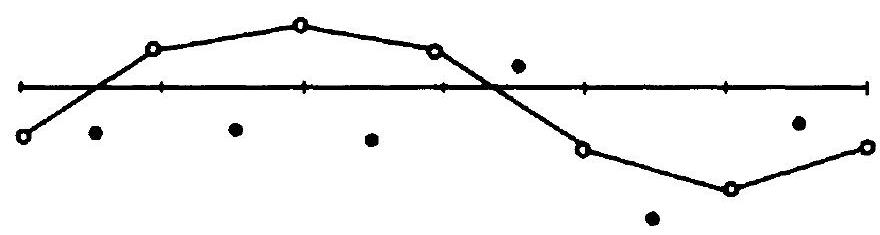
\includegraphics[max width=\textwidth]{2023_10_10_f3de0b9400b097aecf14g-048(1)}
\end{center}
\textbf{Figure 3.3} (a) If the exact error on $\Omega^h$ (indicated by $\circ$ and $\bullet$ ) is smooth, an interpolant of the coarse-grid error $\mathbf{e}^{2 h}$ (solid line connecting $\circ$ points) should give a good representation of the exact error. (b) If the exact error on $\Omega^h$ (indicated by $\circ$ and $\bullet$ ) is oscillatory, an interpolant of the coarse-grid error $\mathbf{e}^{2 h}$ (solid line connecting $\circ$ points) may give a poor representation of the exact error.\\ \\
Assume also that a coarse-grid approximation to the error has been determined on $\Omega^{2 h}$ and that this approximation is exact at the coarse-grid points. When this coarse grid approximation is interpolated to the fine grid, the interpolant is also smooth. Therefore, we expect a relatively good approximation to the fine-grid error, as shown in Fig. 3.3(a). By contrast, if the "real" error is oscillatory, even a very good coarse-grid approximation may produce an interpolant that is not very accurate. This situation is shown in Fig. 3.3(b). \\ \\
Thus, interpolation is most effective when the error is smooth. Because interpolation is necessary for both nested iteration and the correction scheme, we may conclude that these two processes are most effective when the error is smooth. As we will see shortly, these processes provide a fortunate complement to relaxation, which is most effective when the error is oscillatory.
For two-dimensional problems, the interpolation operator may be defined in a similar way. If we let $I_{2 h}^{h} \mathbf{v}^{2 h}=\mathrm{v}^{h}$, then the components of $\mathrm{v}^{h}$ are given by:
$$
\begin{cases}
v_{2 i, 2 j}^{h} & =v_{i j}^{2 h} \\
v_{2 i+1,2 j}^{h} & =\frac{1}{2}\left(v_{i j}^{2 h}+v_{i+1, j}^{2 h}\right) \\
v_{2 i, 2 j+1}^{h} & =\frac{1}{2}\left(v_{i j}^{2 h}+v_{i, j+1}^{2 h}\right) \\
v_{2 i+1,2 j+1}^{h} & =\frac{1}{4}\left(v_{i j}^{2 h}+v_{i+1, j}^{2 h}+v_{i, j+1}^{2 h}+v_{i+1, j+1}^{2 h}\right), \quad 0 \leq i, j \leq \frac{n}{2}-1 .
\end{cases}
$$
The second class of intergrid transfer operations involves moving vectors from a fine grid to a coarse grid. They are generally called restriction operators and are denoted by $I_{h}^{2 h}$. The most obvious restriction operator is injection. It is defined by $I_{h}^{2 h} \mathbf{v}^{h}=\mathrm{v}^{2 h}$, where:
$$
v_{j}^{2 h}=v_{2 j}^{h}
$$
\begin{center}
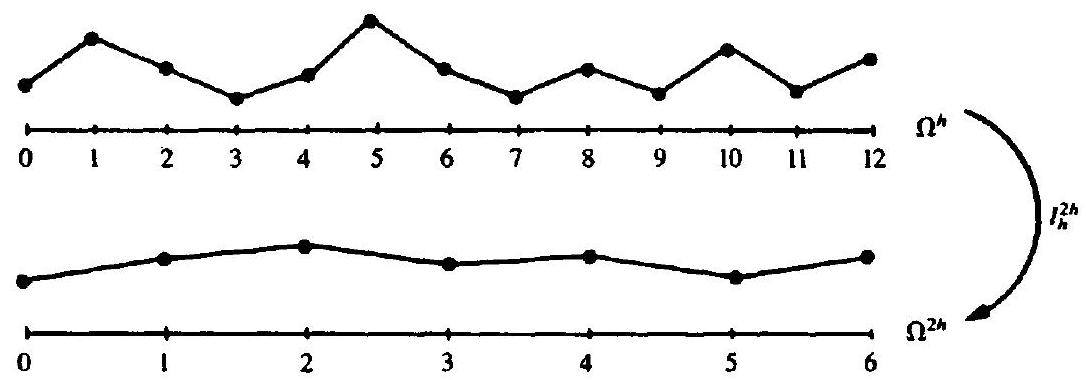
\includegraphics[max width=\textwidth]{2023_10_10_f3de0b9400b097aecf14g-049}
\end{center}
\textbf{Figure 3.4}: Restriction by full weighting of a fine-grid vector to the coarse grid. \\ \\
In other words, with injection, the coarse-grid vector simply takes its value directly from the corresponding fine-grid point. An alternate restriction operator, called full weighting, is defined by $I_{h}^{2 h} \mathbf{v}^{h}=$ $\mathbf{v}^{2 h}$, where:
$$
v_{j}^{2 h}=\frac{1}{4}\left(v_{2 j-1}^{h}+2 v_{2 j}^{h}+v_{2 j+1}^{h}\right), \quad 1 \leq j \leq \frac{n}{2}-1
$$
As Fig. 3.4 shows, the values of the coarse-grid vector are weighted averages of values at neighboring fine-grid points.
In the discussion that follows, we use full weighting as a restriction operator. However, in some instances, injection may be the better choice. \\ \\
The full weighting operator is a linear operator from $\mathbb{R}^{n-1}$ to $\mathbb{R}^{\frac{n}{2}-1}$. It has a rank of $\frac{n}{2}-1$ and a null space of dimension $\frac{n}{2}$.
One reason for our choice of full weighting as a restriction operator is the important fact that:
$$
I_{2 h}^{h}=c\left(I_{h}^{2 h}\right)^{T}, \quad c \in \mathbb{R} .
$$
The fact that the interpolation operator and the full weighting operator are transposes of each other up to a constant is called a variational property and will soon be of importance.
For the sake of completeness, we give the full weighting operator in two dimensions. It is just an averaging of the fine-grid nearest neighbors. Letting $I_{h}^{2 h} \mathbf{v}^{h}=\mathbf{v}^{2 h}$, we have that:
\begin{flalign*}
v_{i j}^{2 h}=\frac{1}{16}\left[v_{2 i-1,2 j-1}^{h}\right. & +v_{2 i-1,2 j+1}^{h}+v_{2 i+1,2 j-1}^{h}+v_{2 i+1,2 j+1}^{h} \\
& +2\left(v_{2 i, 2 j-1}^{h}+v_{2 i, 2 j+1}^{h}+v_{2 i-1,2 j}^{h}+v_{2 i+1,2 j}^{h}\right) 
 \left.+4 v_{2 i, 2 j}^{h}\right], \quad 1 \leq i, j \leq \frac{n}{2}-1
\end{flalign*}
We now have a well-defined way to transfer vectors between fine and coarse grids. Therefore, we can return to the correction scheme and make it precise. To do this, we define the following two-grid correction scheme.

\section*{Two-Grid Correction Scheme}
$$
\mathbf{v}^{h} \leftarrow M G\left(\mathbf{v}^{h}, \mathbf{f}^{h}\right)
$$

\begin{itemize}
  \item Relax $\nu_{1}$ times on $A^{h} \mathbf{u}^{h}=\mathbf{f}^{h}$ on $\Omega^{h}$ with initial guess $\mathbf{v}^{h}$.

  \item Compute the fine-grid residual $\mathbf{r}^{h}=\mathbf{f}^{h}-A^{h} \mathbf{v}^{h}$ and restrict it to the coarse grid by $\mathbf{r}^{2 h}=I_{h}^{2 h} \mathbf{r}^{h}$.

  \item Solve $A^{2 h} \mathbf{e}^{2 h}=\mathbf{r}^{2 h}$ on $\Omega^{2 h}$.

  \item Interpolate the coarse-grid error to the fine grid by $\mathbf{e}^{h}=I_{2 h}^{h} \mathbf{e}^{2 h}$ and correct the fine-grid approximation by $\mathbf{v}^{h} \leftarrow \mathbf{v}^{h}+\mathbf{e}^{h}$.

  \item Relax $\nu_{2}$ times on $A^{h} \mathbf{u}^{h}=\mathbf{f}^{h}$ on $\Omega^{h}$ with initial guess $\mathbf{v}^{h}$.

\end{itemize}
This procedure is simply the original correction scheme, now refined by the use of the inter-grid transfer operators. We relax on the fine grid until it ceases to be worthwhile. In practice, $\nu_{1}$ is often 1, 2, or 3. The residual of the current approximation is computed on $\Omega^{h}$ and then transferred by a restriction operator to the coarse grid. As it stands, the procedure calls for the exact solution of the residual equation on $\Omega^{2 h}$, which may not be possible. However, if the coarse-grid error can at least be approximated, it is then interpolated up to the fine grid, where it is used to correct the fine-grid approximation. This is followed by $\nu_{2}$ additional fine-grid relaxation sweeps. \\ \\
Several comments are in order. First, notice that the superscripts $h$ or $2 h$ are essential to indicate the grid on which a particular vector or matrix is defined. Second, all of the quantities in the above procedure are well defined except for $A^{2 h}$. For the moment, we take $A^{2 h}$ simply to be the result of discretizing the problem on $\Omega^{2 h}$. Finally, the integers $\nu_{1}$ and $\nu_{2}$ are parameters in the scheme that control the number of relaxation sweeps before and after visiting the coarse grid. They are usually fixed at the start, based on either theoretical considerations or on past experimental results.\\ \\
It is important to appreciate the complementarity at work in the process. Relaxation on the fine grid eliminates the oscillatory components of the error, leaving a relatively smooth error. Assuming the residual equation can be solved accurately on $\Omega^{2 h}$, it is still important to transfer the error accurately back to the fine grid. Because the error is smooth, interpolation should work very well and the correction of the fine-grid solution should be effective. \\ \\
One more point needs to be addressed: what initial guess do we use for $v^{2 h}$ on the first visit to $\Omega^{2 h}$ ? Because there is presumably no information available about the solution, $\mathbf{u}^{2 h}$, we simply choose $\mathbf{v}^{2 h}=0$. Here then is the two-grid correction scheme, now imbedded within itself. We assume that there are $l>1$ grids with grid spacings $h, 2 h, 4 h, \ldots, L h=2^{l-1} h$.

\section*{V-Cycle Scheme}
\begin{itemize}
\item $\mathbf{v}^h \leftarrow V^h\left(\mathbf{v}^h, \mathbf{f}^h\right)$
\begin{itemize}
\item Relax on $A^h \mathbf{u}^h=\mathrm{f}^h \ \nu_1$ times with initial guess $\mathbf{v}^h$.
\item Compute $\mathbf{f}^{2 h}=I_h^{2 h} \mathbf{r}^h$.
\begin{itemize}
\item Relax on $A^{2 h} \mathbf{u}^{2 h}=\mathbf{f}^{2 h} \ \nu_1$ times with initial guess $\mathbf{v}^{2 h}=\mathbf{0}$.
\item Compute $\mathbf{f}^{4 h}=I_{2 h}^{4 h} \mathbf{r}^{2 h}$.
\begin{itemize}
\item Relax on $A^{4 h} \mathbf{u}^{4 h}=\mathbf{f}^{4 h} \ \nu_1$ times with initial guess $\mathbf{v}^{4 h}=\mathbf{0}$.
\item Compute $\mathbf{f}^{8 h}=I_{4 h}^{8 h} \mathbf{r}^{4 h}$.
\item Solve $A^{L h} \mathbf{u}^{L h}=\mathbf{f}^{L h}$.
\end{itemize}
\item Correct $\mathbf{v}^{4 h} \leftarrow \mathbf{v}^{4 h}+I_{8 h}^{4 h} \mathbf{v}^{8 h}$.
\item Relax on $A^{4 h} \mathbf{u}^{4 h}=\mathrm{f}^{4 h} \ \nu_2$ times with initial guess $\mathbf{v}^{4 h}$.
\end{itemize}
\item Correct $\mathbf{v}^{2 h} \leftarrow \mathbf{v}^{2 h}+I_{4 h}^{2 h} \mathbf{v}^{4 h}$.
\item Relax on $A^{2 h} \mathbf{u}^{2 h}=\mathbf{f}^{2h} \ v_{2}$ times with initial guess $\mathbf {v}^{2h}$.
\end{itemize}
\item Correct $\mathbf{v}^h \leftarrow \mathbf{v}^h+I_{2 h}^h \mathbf{v}^{2 h}$.
\item Relax on $A^h \mathbf{u}^h=\mathbf{f}^h \nu_2$ times with initial guess $\mathbf{v}^h$.
\end{itemize}
The algorithm telescopes down to the coarsest grid, which can consist of one or a few interior grid points, then works its way back to the finest grid. Figure 3.6(a) shows the schedule for the grids in the order in which they are visited. Because of the pattern in this diagram, this algorithm is called the $V$-cycle. It is our first true multigrid method. \\
Not surprisingly, the V-cycle has a compact recursive definition, which is given as follows.


\section*{V-Cycle Scheme (Recursive Definition)}
To facilitate the description of this procedure, some economy of notation is desirable. The same notation is used for the computer implementation of the resulting algorithm. We call the right-side vector of the residual equation $\mathbf{f}^{2 h}$, rather than $\mathbf{r}^{2 h}$, because it is just another right-side vector. Instead of calling the solution of the residual equation $\mathbf{e}^{2 h}$, we use $\mathbf{u}^{2 h}$ because it is just a solution vector. We can then use $\mathbf{v}^{2 h}$ to denote approximations to $\mathbf{u}^{2 h}$. These changes simplify the notation, but it is still important to remember the meaning of these variables. \\ \\
One more point needs to be addressed: what initial guess do we use for $\mathbf{v}^{2 h}$ on the first visit to $\Omega^{2 h}$ ? Because there is presumably no information available about the solution, $\mathbf{u}^{2 h}$, we simply choose $\mathbf{v}^{2 h}=0$. Here then is the two-grid correction scheme, now imbedded within itself. We assume that there are $l>1$ grids with grid spacings $h, \ 2 h, \  4 h, \ \ldots, L h=2^{l-1} h$.\\ \\ 
\begin{enumerate}
  \item Relax $\nu_{1}$ times on $A^{h} \mathbf{u}^{h}=\mathbf{f}^{h}$ with a given initial guess $\mathbf{v}^{h}$.

  \item If $\Omega^{h}=$ coarsest grid, then go to step 4 .
\end{enumerate}

Else

$$
\begin{aligned}
& \mathbf{f}^{2 h} \leftarrow I_{h}^{2 h}\left(\mathbf{f}^{h}-A^{h} \mathbf{v}^{h}\right) \\
& \mathbf{v}^{2 h} \leftarrow \mathbf{0} \\
& \mathbf{v}^{2 h} \leftarrow V^{2 h}\left(\mathbf{v}^{2 h}, \mathbf{f}^{2 h}\right)
\end{aligned}
$$

\begin{enumerate}
  \setcounter{enumi}{2}
  \item Correct $\mathrm{v}^{h} \leftarrow \mathrm{v}^{h}+I_{2 h}^{h} \mathrm{v}^{2 h}$.

  \item Relax $\nu_{2}$ times on $A^{h} \mathbf{u}^{h}=\mathbf{f}^{h}$ with initial guess $\mathbf{v}^{h}$.
\end{enumerate}
  The V-cycle is just one of a family of multigrid cycling schemes. The entire family is called the $\mu$-cycle method and is defined recursively by the following.
\section*{$\mu$-Cycle Scheme}
$$
\mathbf{v}^{h} \leftarrow M \mu^{h}\left(\mathbf{v}^{h}, \mathrm{f}^{h}\right)
$$

\begin{enumerate}
  \item Relax $\nu_{1}$ times on $A^{h} \mathbf{u}^{h}=\mathrm{f}^{h}$ with a given initial guess $\mathbf{v}^{h}$.

  \item If $\Omega^{h}=$ coarsest grid, then go to step 4 .

\end{enumerate}

Else

$$
\begin{aligned}
& \mathbf{f}^{2 h} \leftarrow I_{h}^{2 h}\left(\mathbf{f}^{h}-A^{h} \mathbf{v}^{h}\right) \\
& \mathbf{v}^{2 h} \leftarrow 0 \\
& \mathbf{v}^{2 h} \leftarrow M \mu^{2 h}\left(\mathbf{v}^{2 h}, \mathbf{f}^{2 h}\right) \mu \text { times. }
\end{aligned}
$$

\begin{enumerate}
  \setcounter{enumi}{2}
  \item Correct $\mathbf{v}^{h} \leftarrow \mathbf{v}^{h}+I_{2 h}^{h} \mathbf{v}^{2 h}$.

  \item Relax $\nu_{2}$ times on $A^{h} \mathbf{u}^{h}=\mathbf{f}^{h}$ with initial guess $\mathbf{v}^{h}$.

\end{enumerate}
In practice, only $\mu=1$ (which gives the V-cycle) and $\mu=2$ are used. Figure 3.6(b) shows the schedule of grids for $\mu=2$ and the resulting $W$-cycle. We refer to a $\mathrm{V}$-cycle with $\nu_{1}$ relaxation sweeps before the correction step and $\nu_{2}$ relaxation sweeps after the correction step as a $\mathrm{V}\left(\nu_{1}, \nu_{2}\right)$-cycle, with a similar notation for W-cycles. \\ \\
We originally stated that two ideas would lead to multigrid. So far we have developed only the correction scheme. The nested iteration idea has yet to be explored. Recall that nested iteration uses coarse grids to obtain improved initial guesses for fine-grid problems. In looking at the V-cycle, we might ask how to obtain an informed initial guess for the first fine-grid relaxation. Nested iteration would suggest solving a problem on $\Omega^{2 h}$. But how can we obtain a good initial guess for the $\Omega^{2 h}$ problem? Nested iteration sends us to $\Omega^{4 h}$. Clearly, we are on another recursive path that leads to the coarsest grid. \\ \\         
The algorithm that joins nested iteration with the V-cycle is called the full multigrid $V$-cycle (FMG). Given first in explicit terms, it appears as follows.

\section*{Full Multigrid V-Cycle}
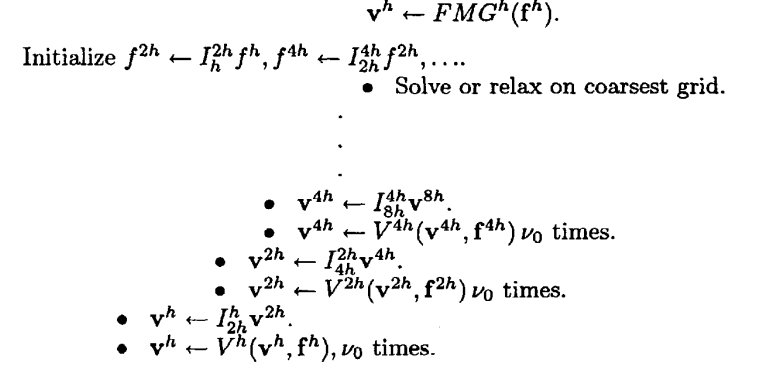
\includegraphics[scale=0.6]{images/FMVC1.png} \\ \\
We initialize the coarse-grid right sides by transferring $\mathbf{f}^{h}$ from the fine grid. Another option is to use the original right-side function $f$. The cycling parameter, $\nu_{0}$, sets the number of $\mathbf{V}$-cycles done at each level. It is generally determined by a previous numerical experiment; $\nu_{0}=1$ is the most common choice. Expressed recursively, the algorithm has the following compact form.
\section*{Full Multigrid V-Cycle (Recursive Form)}
$$
\mathbf{v}^{h} \leftarrow F M G^{h}\left(\mathbf{f}^{h}\right)
$$

\begin{enumerate}
  \item If $\Omega^{h}=$ coarsest grid, set $\mathbf{v}^{h} \leftarrow \mathbf{0}$ and go to step 3 .
\end{enumerate}

Else

$$
\begin{aligned}
& \mathbf{f}^{2 h} \leftarrow I_{h}^{2 h}\left(\mathbf{f}^{h}\right) \\
& \mathbf{v}^{2 h} \leftarrow F M G^{2 h}\left(\mathbf{f}^{2 h}\right) .
\end{aligned}
$$

\begin{enumerate}
  \setcounter{enumi}{1}
  \item Correct $\mathbf{v}^{h} \leftarrow I_{2 h}^{h} \mathbf{v}^{2 h}$.

  \item $\mathbf{v}^{h} \leftarrow V^{h}\left(\mathbf{v}^{h}, \mathbf{f}^{h}\right) \nu_{0}$ times.

\end{enumerate}
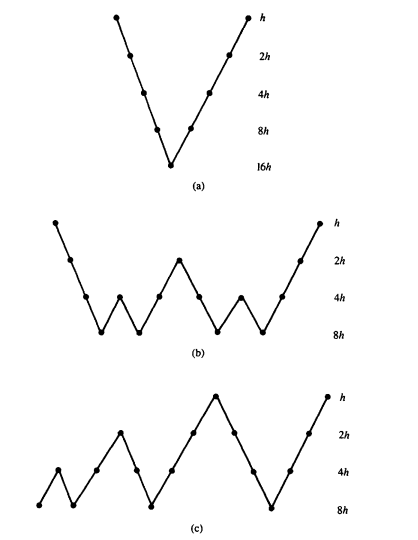
\includegraphics[]{images/MMM.png}\\
\textbf{Figure 3.6} Schedule of grids for (a) V-cycle, (b) W-cycle, and (c) FMG scheme,
all on four levels.\\ \\
Figure 3.6(c) shows the schedule of grids for FMG with $\nu_{0}=1$. Each Vcycle is preceded by a coarse-grid $\mathrm{V}$-cycle designed to provide the best initial guess possible. As we will see, the extra work done in these preliminary V-cycles is not only inexpensive (Exercise 8 ), but easily pays for itself.\\ \\ 
Full multigrid is the complete knot into which the many threads of the preceding pages are tied. It is a remarkable synthesis of ideas and techniques that individually have been well known and used for a long time. Taken alone, many of these ideas have serious defects. Full multigrid is a technique for integrating them so that they can work together in a way that overcomes these limitations. The result is a very powerful algorithm.

\chapter{Algebraic Multigrid Methods}
This chapter follows closely the eighth chapter of the following book: "A Multigrid Tutorial: Second Edition", by  William L. Briggs, Van Emden Henson, Steve F. McCormick. It is recommended to read it to gain a deeper understanding. \\ \\
Can we apply multigrid techniques when there is no grid? Suppose we have relationships among the unknowns that are similar to those in the model problem, but the physical locations of the unknowns are themselves unknown (or immaterial). Can we hope to apply the tools we have developed? A related question is if it is possible to apply multigrid in the case where grid locations are known but may be highly unstructured or irregular, making the selection of a coarse grid problematic? These are the problems that are addressed by a technique known as algebraic multigrid, or AMG. \\ \\
For any multigrid algorithm, the same fundamental components are required. There must be a sequence of grids, intergrid transfer operators, a relaxation (smoothing) operator, coarse-grid versions of the fine-grid operator, and a solver for the coarsest grid.\\ \\
Let us begin by deciding what we mean by a grid. Throughout this chapter, we look to standard multigrid (which we refer to as the geometric case) to guide us in defining AMG components. In the geometric case, the unknown variables $u_{i}$ are defined at known spatial locations (grid points) on a fine grid. We then select a subset of these locations as a coarse grid. As a consequence, a subset of the variables $u_{i}$ is used to represent the solution on the coarse grid. For AMG, by analogy, we seek a subset of the variables $u_{i}$ to serve as the coarse-grid unknowns. A useful point of view, then, is to identify the grid points with the indices of the unknown quantities. Hence, if the problem to be solved is $A \mathbf{u}=\mathbf{f}$ and then the fine-grid points are just the indices $\{1,2, \ldots, n\}$.
$$
\mathbf{u}=\left[\begin{array}{c}
u_{1} \\
u_{2} \\
\vdots \\
u_{n}
\end{array}\right]
$$
Having defined the grid points, the connections within the grid are determined by the undirected adjacency graph of the matrix $A$. Letting the entries of $A$ be $a_{i j}$, we associate the vertices of the graph with the grid points and draw an edge between the $i$-th and $j$-th vertices if either $a_{i j} \neq 0$ or $a_{j i} \neq 0$. The connections in the grid are the edges in the graph; hence, the grid is entirely defined by the matrix A. For example:
$$
A=\left[\begin{array}{llllll}
X & X & & X & X & \\
X & X & X & X & & \\
& X & X & X & X & X \\
X & X & X & X & & \\
X & & X & & X & X \\
& & X & & X & X
\end{array}\right]
$$
Now that we can represent the fine grid, how do we select a coarse grid? With standard multigrid methods, smooth functions are geometrically or physically smooth; they have a low spatial frequency. In these cases, we assume that relaxation smooths the error and we select a coarse grid that represents smooth functions accurately. We then choose intergrid operators that accurately transfer smooth functions between grids.\\ \\
With AMG, the approach is different. We first select a relaxation scheme that allows us to determine the nature of the smooth error. Because we do not have access to a physical grid, the sense of smoothness must be defined algebraically. The next step is to use this sense of smoothness to select coarse grids, which will be subsets of the unknowns. A related issue is the choice of intergrid transfer operators that allow for effective coarsening. Finally, we select the coarse-grid versions of the operator $A$, so that coarse-grid correction has the same effect that it has in geometric multigrid: it must eliminate the error components in the range of the interpolation operator.

\section*{Algebraic Smoothness}
Having chosen a relaxation scheme, the crux of the problem is to determine what is meant by smooth error. If the problem provides no geometric information (for example, true grid point locations are unknown), then we cannot simply examine the Fourier modes of the error. Instead, we must proceed by analogy. In the geometric case, the most important property of smooth error is that it is not effectively reduced by relaxation. Thus, we now define smooth error loosely to be any error that is not reduced effectively by relaxation. \\ \\
That was simple. Of course, we still need to figure out exactly what this definition means. To do this in the simplest case, we focus on weighted point Jacobi relaxation. We also assume that $A$ is a symmetric $M$-matrix: it is symmetric $\left(A^{T}=A\right)$ and positive-definite $\left(\mathbf{u}^{T} A \mathbf{u}>0\right.$ for all $\left.\mathbf{u} \neq 0\right)$ and has positive diagonal entries and non-positive off-diagonal entries. These properties are shared by matrices arising from the discretization of many (not all) scalar elliptic differential equations. These assumptions are not necessary for AMG to work. However, the original theory of AMG was developed for symmetric M-matrices, and if $A$ is far from being an M-matrix, it is less likely that standard AMG will be effective in solving the problem. \\ \\
By our definition, algebraic smoothness means that the size of $\mathbf{e}^{i+1}$ is not significantly less than that of $\mathbf{e}^{i}$. We need to be more specific about the concept of size. A natural choice is to measure the error in the $A$-norm, which is induced by the $A$-inner product. We have that:
$$
\|\mathbf{e}\|_{A}=(A \mathbf{e}, \mathbf{e})^{1 / 2}
$$
It can be derived that it is possible to write this condition loosely as:
$$
A \mathbf{e} \approx \mathbf{0}
$$
and read it as meaning that smooth error has relatively small residuals.

\section*{Influence and Dependence}
Most of AMG rests on two fundamental concepts. We have just discussed the first concept, namely, smooth error. The second important concept is that of strong dependence or strong influence. Because of the dominance of the diagonal entry ($A$ is an M-matrix), we associate the $i$- th equation with the $i$-th unknown. The job of the $i$-th equation is to determine the value of $u_{i}$. Of course, it usually takes all of the equations to determine any given variable precisely. Nevertheless, our first task is to determine which other variables are most important in the $i$-th equation, which $u_{j}$ are most important in the $i$-th equation in determining $u_{i}$? \\ \\
One answer to this question lies in the following observation: if the coefficient, $a_{i j}$, which multiplies $u_{j}$ in the $i$-th equation, is large relative to the other coefficients in the $i$-th equation, then a small change in the value of $u_{j}$ has more effect on the value of $u_{i}$ than a small change in other variables in the $i$-th equation. Intuitively, it seems logical that a variable whose value is instrumental in determining the value for $u_{i}$ would be a good value to use in the interpolation of $u_{i}$. Hence, such a variable (point) should be a candidate for a coarse-grid point. This observation suggests the following definition.\\ \\
\textbf{Definition 1.} Given a threshold value $0<\theta \leq 1$, the variable (point) $u_{i}$ strongly depends on the variable (point) $u_{j}$ if
$$
-a_{i j} \geq \theta \max _{k \neq i}\left\{-a_{i k}\right\}
$$
This says that grid point $i$ strongly depends on grid point $j$ if the coefficient $a_{i j}$ is comparable in magnitude to the largest off-diagonal coefficient in the $i$ th equation. We can state this definition from another perspective. \\ \\
\textbf{Definition 2.} If the variable $u_{i}$ strongly depends on the variable $u_{j}$, then the variable $u_{j}$ strongly influences the variable $u_{i}$. \\ \\ 
With the twin concepts of smooth error and strong influence/dependence in hand, we can return to the task of defining the multigrid components for AMG. As with any multigrid algorithm, we begin by defining a two-grid algorithm, then proceed to multigrid by recursion. Having defined the relaxation scheme, we have several tasks before us:
\begin{itemize}

 \item  Select a coarse grid so that the smooth components can be represented accurately;
 
  \item Define an interpolation operator so that the smooth components can be accurately transferred from the coarse grid to the fine grid; 

  \item Define a restriction operator and a coarse-grid version of $A$ using the variational properties.

\end{itemize}

\section*{Defining the Interpolation Operator}
Assume for the moment that we have already designated the coarse-grid points. This means that we have a partitioning of the indices $\{1,2, \ldots, n\}=C \cup F$, where the variables (points) corresponding to $i \in C$ are the coarse-grid variables. These coarse-grid variables are also fine-grid variables and the indices $i \in F$ represent those variables that are only fine-grid variables. Next, suppose that $e_{i}, \ i \in C$, is a set of values on the coarse grid representing a smooth error that must be interpolated to the fine grid, $C \cup F$. What do we know about $e_{i}$ that allows us to build an interpolation operator that is accurate? With geometric multigrid, we use linear interpolation between the coarse grid points. With an unstructured, or perhaps nonexistent, grid, the answer is not so obvious. \\ \\
If a $C$-point $j$ strongly influences an $F$-point $i$, then the value $e_{j}$ contributes heavily to the value of $e_{i}$ in the $i$-th (fine-grid) equation. It seems reasonable that the value $e_{j}$ in the coarse-grid equation could therefore be used in an interpolation formula to approximate the fine-grid value $e_{i}$. This idea can be strengthened by noting that the following bound must hold for smooth error on average, that is, for most $i$:
$$
\sum_{j \neq i}\left(\frac{\left|a_{i j}\right|}{a_{i i}}\right)\left(\frac{e_{i}-e_{j}}{e_{i}}\right)^{2} \ll 1, \quad 1 \leq i \leq n
$$
The left side of the inequality is a sum of products of non-negative terms. These products must be very small, which means that one or both of the factors in each product must be small. But if $e_{i}$ strongly depends on $e_{j}$, we know that $-a_{i j}$ could be comparable to $a_{i i}$. Therefore, for these strongly influencing $e_{j}$'s, it must be true that $e_{i}-e_{j}$ is small, so $e_{j} \approx e_{i}$.\\ \\
We describe this by saying that smooth error varies slowly in the direction of strong connection. Thus, we have a justification for the idea that the fine-grid quantity $u_{i}$ can be interpolated from the coarse-grid quantity $u_{j}$ if $i$ strongly depends on $j$.\\ \\
For each fine-grid point $i$, we define $N_{i}$, the neighborhood of $i$, to be the set of all points $j \neq i$ such that $a_{i j} \neq 0$. These points can be divided into three categories:
\begin{itemize}
  \item The neighboring coarse-grid points that strongly influence $i$. This is the coarse interpolatory set for $i$, denoted by $C_{i}$.

  \item The neighboring fine-grid points that strongly influence $i$, denoted by $D_{i}^{s}$; and

  \item The points that do not strongly influence $i$, denoted by $D_{i}^{w}$; this set may contain both coarse- and fine-grid points; it is called the set of weakly connected neighbors. 
\end{itemize}
The goal is to define the interpolation operator $I_{2 h}^{h}$ (although physical grids may not be present, we continue to denote fine-grid quantities by $h$ and coarse-grid quantities by $2 h$ ). We require that the $i$ th component of $I_{2 h}^{h} \mathbf{e}$ be given by:
$$
\left(I_{2 h}^{h} \mathbf{e}\right)_{i}=\left\{\begin{aligned}
e_{i} & \text { if } i \in C, \\
\sum_{j \in C_{i}} \omega_{i j} e_{j} & \text { if } i \in F,
\end{aligned}\right.
$$
where the interpolation weights, $\omega_{i j}$, must now be determined.\\ \\
Recall that the main characteristic of smooth error is that the residual is small: $\mathbf{r} \approx 0$. We can write the $i$-th component of this condition as:
$$
a_{i i} e_{i} \approx-\sum_{j \in N_{i}} a_{i j} e_{j}
$$
Splitting the sum into its component sums over the coarse interpolatory set, $C_{i}$, the fine-grid points with strong influence, $D_{i}^{s}$, and the weakly connected neighbors, $D_{i}^{w}$, we have:
$$
a_{i i} e_{i} \approx-\sum_{j \in C_{i}} a_{i j} e_{j}-\sum_{j \in D_{i}^{s}} a_{i j} e_{j}-\sum_{j \in D_{i}^{w}} a_{i j} e_{j}
$$
To determine the $\omega_{i j}$, we need to replace the $e_{j}$ in the second and third sums on the right side of the last equation with approximations in terms of $e_{i}$ or $e_{j}$, where $j \in C_{i}$.\\ \\
Consider the third sum over points that are weakly connected to point $i$. We distribute these terms to the diagonal coefficient; that is, we simply replace $e_{j}$ in the rightmost sum by $e_{i}$, giving:
$$
\left(a_{i i}+\sum_{j \in D_{i}^{w}} a_{i j}\right) e_{i} \approx-\sum_{j \in C_{i}} a_{i j} e_{j}-\sum_{j \in D_{i}^{s}} a_{i j} e_{j} \ \ \ (4.1)
$$
We can justify this distribution in the following way. Suppose we have underestimated the dependence, so that $e_{i}$ does depend strongly on the value of the points in $D_{i}^{w}$. Then the fact that smooth error varies slowly in the direction of strong dependence means that $e_{i} \approx e_{j}$ and the distribution to the diagonal makes sense. Alternatively, suppose the value of $e_{i}$ does not depend strongly on the points in $D_{i}^{w}$. Then the corresponding value of $a_{i j}$ will be small and any error committed in making this assignment will be relatively insignificant.\\ \\
Treating the second sum over $D_{i}^{s}$ is a bit more complicated because we must be more careful with these strong connections. We might simply distribute these terms to the diagonal, and, indeed, this would work nicely for many problems. However, experience has shown that it is better to distribute the terms in $D_{i}^{s}$ to $C_{i}$. Essentially, we want to approximate the $e_{j}$'s in this sum with weighted sums of the $e_{k}$ for $k \in C_{i}$. That is, we want to replace each $e_{j}$, where $j$ is a fine-grid point that strongly influences $i$, with a linear combination of values of $e_{k}$ from the coarse interpolatory set of the point $i$. We do this, for each fixed $j \in D_{i}^{s}$, by making the approximation:
$$
e_{j} \approx \frac{\sum_{k \in C_{i}} a_{j k} e_{k}}{\sum_{k \in C_{i}} a_{j k}} \ \  \ (4.2)
$$
The numerator is appropriate because the $e_{j}$ are strongly influenced by the $e_{k}$ in proportion to the matrix entries $a_{j k}$. The denominator is chosen to ensure that the approximation interpolates constants exactly. Notice that this approximation requires that if $i$ and $j$ are any two strongly connected fine-grid points, then they must have at least one point common to their coarse interpolatory sets $C_{i}$ and $C_{j}$.
If we now substitute (4.2) into (4.1) and engage in a spate of algebra, we find that the interpolation weights are given by
$$
\omega_{i j}=-\frac{a_{i j}+\sum_{m \in D_{i}^{s}}\left(\frac{a_{i m} a_{m j}}{\sum_{k \in C_{i}} a_{m k}}\right)}{a_{i i}+\sum_{n \in D_{i}^{w}} a_{i n}} .
$$
In the context of Algebraic Multigrid (AMG) methods, $\omega_{ij}$ represents an element of the interpolation matrix, which is crucial in the process of transferring information between different grid levels. Each $\omega_{ij}$ essentially determines the weight or influence of the coarse grid variable $u_j$ on the fine grid variable $u_i$ during the interpolation process. These weights are not related to the frequency of any quantity, but instead, they are computed based on the strength of connections between different variables and the smoothness of the error. The interpolation matrix, populated with these $\omega_{ij}$ weights, is used to approximate the values of the fine grid variables using the values of the coarse grid variables. Therefore, $\omega_{ij}$ plays a key role in the effectiveness and accuracy of the AMG method.

\section*{Selecting the Coarse Grid}
The preceding discussion of the interpolation operator assumed that we had already designated points of the coarse grid. We must now turn our attention to this critical task. We use the twin concepts of strong influence/dependence and smooth error, just as we did in defining interpolation. As in the geometric problem, we rely on the fundamental premise that the coarse grid must be one with the following characteristics:
\begin{itemize}
  \item On which smooth error can be approximated accurately;

  \item From which smooth functions can be interpolated accurately;

  \item It has substantially fewer points than the fine grid, so that the residual problem may be solved with relatively little expense. 
\end{itemize}
The basic idea is straightforward. By examining the suitability of each grid point to be a point of one of the $C_{i}$ sets, we make an initial partitioning of the grid points into $C$-and $F$-points. Then, as the interpolation operator is constructed, we make adjustments to this partitioning, changing points initially chosen as $F$-points to be $C$-points in order to ensure that the partitioning conforms to certain heuristic rules.\\ \\
Before we can describe the coarsening process in detail, we need to make two more definitions and to introduce these heuristics. Denote by $S_{i}$ the set of points that strongly influence $i$, the points on which the point $i$ strongly depends. Also denote by $S_{i}^{T}$ the set of points that strongly depend on the point $i$. Armed with these definitions, we describe two heuristic criteria that guide the initial selection of the $C$-points:\\ \\
\textbf{H-1:} For each $F$-point $i$, every point $j \in S_{i}$ that strongly influences $i$ either should be in the coarse interpolatory set $C_{i}$ or should strongly depend on at least one point in $C_{i}$.\\ \\
\textbf{H-2:} The set of coarse points $C$ should be a maximal subset of all points with the property that no $C$-point strongly depends on another $C$-point. \\ \\
To motivate heuristic H-1, we examine the approximation (4.2) that was made in developing the interpolation formula. Recall that this approximation applies to points $j \in D_{i}^{s}$ that consist of $F$-points strongly influencing the $F$-point $i$. Because $e_{i}$ depends on these points, their values must be represented in the interpolation formula in order to achieve accurate interpolation. But because they have not been chosen as $C$-points, they are represented in the interpolation formula only by distributing their values to points in $C_{i}$ using (4.2). It seems evident that (4.2) will be more accurate if $j$ is strongly dependent on several points in $C_{i}$. However, for the approximation to be made at all, $j$ must be strongly dependent on at least one point in $C_{i}$. Heuristic H-1 simply ensures that this occurs. \\ \\
Heuristic \textbf{H-2} is designed to strike a balance on the size of the coarse grid. Multigrid efficiency is generally controlled by two properties: convergence factor and number of WUs per cycle. If the coarse grid is a large fraction of the total points, then the interpolation of smooth errors is likely to be very accurate, which, in turn, generally produces better convergence factors. However, relatively large coarse grids generally mean a prohibitively large amount of work in doing V-cycles. By requiring that no $C$-point strongly depends on another, $\mathbf{H-2}$ controls the size of the coarse grid because $C$-points tend to be farther apart. By requiring $C$ to be a maximal subset (that is, no other point can be added to $C$ without violating the ban on mutual strong dependence), $\mathbf{H-2}$ ensures that $C$ is big enough to produce good convergence factors.\\ \\
It is not always possible to enforce both \textbf{H-1} and \textbf{H-2}. Because the interpolation formula depends on $\mathbf{H-1}$ being satisfied, we choose to enforce \textbf{H-1} rigorously, while using \textbf{H-2} as a guide. While this choice may lead to larger coarse grids than necessary, experience shows that this trade-off between accuracy and expense is generally worthwhile. \\ \\
The basic coarse-point selection algorithm proceeds in two passes. We first make an initial coloring of the grid points by choosing a preliminary partition into $C$ and $F$-points. The goal in the first pass is to create a set of $C$-points that have good approximation properties and also tend to satisfy  \textbf{H-2}. Once the initial assignments have been made, we make a second pass, changing initial $F$-points to $C$-points as necessary to enforce \textbf{H-1}.

\section*{The Coloring Scheme}
The first pass begins by assigning to each point $i$ a measure of its potential quality as a $C$-point. There are several ways we can make this assessment, but the simplest is to count the number of other points strongly influenced by $i$. Because those points are the members of $S_{i}^{T}$, this count, $\lambda_{i}$, is the cardinality of $S_{i}^{T}$. Once the measures $\lambda_{i}$ have been determined, we select a point with maximum $\lambda_{i}$ value as the first point in $C$. \\ \\
The point we just selected strongly influences several of the other points and should appear in the interpolation formula for each of them. This implies that the points that depend strongly on $i$ should become $F$-points. We therefore assign all points in $S_{i}^{T}$ to $F$, which is permissible because we already have a $C$-point, $i$, that strongly influences them. It is logical to look at other points that strongly influence these new $F$-points as potential $C$-points, because their values could be useful for accurate interpolations. Therefore, for each new $F$-point $j$ in $S_{i}^{T}$, we increment the measure, $\lambda_{k}$, of each unassigned point $k$ that strongly influences $j$, this would be each unassigned member of $k \in S_{j}$.\\ \\
The process is then repeated. A new unassigned point $i$ is found with maximum $\lambda_{i}$ and it is assigned to $C$. The unassigned points $j \in S_{i}^{T}$ are then assigned to $F$ and the measures of the unassigned points in $S_{j}$ are incremented by 1. This process continues until all points have been assigned to $C$ or $F$. \\ \\
It is useful to observe that the coarsening determined by this method depends on several factors. Among the most influential is the order in which the grid points are scanned when seeking the next point with maximal $\lambda$. Because many, if not most, of the grid points will have the maximal value at the start, any of them could be selected as the first coarse point. Once the first point is selected, the rest proceeds as outlined. Again, any time there is more than one point having the maximal value, there are many possible coarsenings. The heuristics ensure that whatever specific coarse grid is obtained, it will have the desired properties: it provides a good representation of smooth error components, while keeping the size of the coarse grid reasonably small.


\section*{Coarse-Grid Operators}
Recall that although physical grids may not be present, we continue to denote fine-grid quantities by $h$ and coarse-grid quantities by $2 h$. Once the coarse grid is chosen and the interpolation operator $I_{2 h}^{h}$ is constructed, the restriction operator $I_{h}^{2 h}$ is defined using the usual variational property:
$$
I_{h}^{2 h}=\left(I_{2 h}^{h}\right)^{T}
$$
The coarse-grid operator is constructed using the Galerkin condition:
$$
A^{2 h}=I_{h}^{2 h} A^{h} I_{2 h}^{h}
$$
The reason for defining interpolation and the coarse operator by these variational principle is that the resulting coarse-grid correction is optimal in the $A^{h}$-norm.

\section*{Cycling Algorithms}
We have now defined all the components necessary to create a two-grid correction algorithm for AMG: a relaxation scheme, a set of coarse-grid points $C$, a coarsegrid operator $A^{2 h}$, and intergrid transfer operators $I_{h}^{2 h}$ and $I_{2 h}^{h}$. Although we have discussed weighted Jacobi, Gauss-Seidel relaxation is often preferred. The two-grid correction algorithm appears exactly as it did for geometric multigrid, as shown below.

\section*{AMG Two-Grid Correction Cycle}
$$
\mathbf{v}^{h} \leftarrow \operatorname{AMG}\left(\mathbf{v}^{h}, \mathbf{f}^{h}\right) .
$$

\begin{itemize}
  \item Relax $\nu_{1}$ times on $A^{h} \mathbf{u}^{h}=\mathbf{f}^{h}$ with initial guess $\mathbf{v}^{h}$.

  \item Compute the fine-grid residual $\mathbf{r}^{h}=\mathbf{f}^{h}-A^{h} \mathbf{v}^{h}$ and restrict it to the coarse grid by $\mathbf{r}^{2 h}=I_{h}^{2 h} \mathbf{r}^{h}$.

  \item Solve $A^{2 h} \mathrm{e}^{2 h}=\mathrm{r}^{2 h}$ on $\Omega^{2 h}$.

  \item Interpolate the coarse-grid error to the fine grid by $\mathrm{e}^{h}=I_{2 h}^{h} \mathrm{e}^{2 h}$ and correct the fine-grid approximation by $\mathbf{v}^{h} \leftarrow \mathbf{v}^{h}+\mathbf{e}^{h}$.

  \item Relax $\nu_{2}$ times on $A^{h} \mathbf{u}^{h}=\mathbf{f}^{h}$ with initial guess $\mathbf{v}^{h}$.

\end{itemize}
Having defined the two-grid correction algorithm, we can define other multigrid cycling schemes for AMG guided by geometric multigrid. For example, to create a V-cycle algorithm, we simply replace the direct solution of the coarse-grid problem with a recursive call to AMG on all grids except the coarsest grid, where we use a direct solver. W-cycles, $\mu$-cycles, and FMG-cycles can also be created by strict analogy to the geometric multigrid case.

\section*{Parallel Coarsening Algorithms}
C-AMG coarsening algorithm is inherently sequential. There are several parallel algorithms (in hypre):

\begin{itemize}
  \item CLJP (Cleary-Luby-Jones-Plassmann): one-pass approach with random numbers to get concurrency.
  \item Falgout-C-AMG on processor interior, then CLJP to finish.
  \item CGC (Griebel, Metsch, Schweitzer): compute several coarse grids on each processor, then solve a global graph problem to select the grids with the best "fit.
\end{itemize}
Other parallel AMG codes use similar approaches.

\section*{Take home message}
   In Algebraic Multigrid (AMG), the construction of the multigrid hierarchy is carried out using only information from the matrix and not from the geometry of the problem. This approach has optimal convergence and good scaling potential with linear complexity. However, exposing high parallelism is not easy at "too coarse" levels. To achieve parallelism, additional restrictions on AMG algorithmic development are necessary. 
\chapter{Domain Decomposition Methods}
\section*{Alternating Schwarz Method}
Consider (an elliptic) partial differential equation of the form:
$$ L u=f \quad \text{in} \Omega=\Omega_{1} \cup \Omega_{2} $$
with boundary condition $u=g$ on $\partial \Omega$.

Given $u^{(0)}$\\ \\ 
1) On $\Omega_1$ solve $\begin{cases}L u_1^{\left(k+\frac{1}{2}\right)}=f & \text { in } \Omega_1 \\ u_1^{\left(k+\frac{1}{2}\right)}=g & \text { in } \partial \Omega_1 \backslash \Gamma_1 \\ u_1^{\left(k+\frac{1}{2}\right)}=u_2^{(k)} & \text { in } \Gamma_1\end{cases}$ \\ \\ \\ \\
2) On $\Omega_2$ solve $\left\{\begin{array}{rlrl}L u_2^{(k+1)} & =f &  \text { in } \Omega_2 \\ u_2^{(k+1)}=g &  \text { in } \partial \Omega_2 \backslash \Gamma_2 \\
u_2^{(k+1)} & =u_1^{\left(k+\frac{1}{2}\right)} &  \text { in } \Gamma_2\end{array}\right.$ \\ \\ \\ \\
3) Define $u^{(k+1)}=\left\{\begin{array}{lr}u_1^{\left(k+\frac{1}{2}\right)} & \text { in } \Omega  \backslash \Omega_2 \\ 
u_2^{(k+1)} & \text { in } \Omega_2\end{array}\right.$\\ \\
Schwarz proposed a method in 1870 to deal with regions for which analytical solutions are not known. This method involves alternating iterations until convergence to the solution on the entire domain. Today, this method is of interest in its discretized form, as it suggests one of two major paradigms for solving PDEs numerically by domain decomposition. The two paradigms are overlapping subdomains (Schwarz) and non-overlapping subdomains (Schur).\\
For $i=1,2$, let $S_{i}$ be set of $n_{i}$ indices of grid points in the interior of $\Omega_{i}$, where $n_{i}=\left|S_{i}\right|$. Because subdomains overlap, $S_{1} \cap S_{2} \neq \varnothing$ and $n_{1}+n_{2}>n$.

\section*{Discretized Schwarz Methods}
 Let $I$ be the set of indices of grid points in the interior of $\Omega$, where $|I|=N$. Because subdomains overlap, $I=\bigcup_{i=1}^m I_i$ and $I_i\cap I_j\neq \emptyset$ for some $i\neq j$. For $i=1,\dots,m$, let $R_i$ be the Boolean restriction matrix such that for any vector $x\in \mathbb{R}^N$, $R_ix$ contains precisely those components of $x$ corresponding to indices in $I_i$ (i.e., those components associated with nodes in $\Omega_i$). \\ \\
Conversely, let $E_i$ be the extension matrix that expands the vector $v_i$ into a vector $v=E_iv_i\in \mathbb{R}^N$, whose components corresponding to indices in $I_i$ are the same as those of $v_i$, and whose remaining components are all zero. The principal submatrices of $A$ corresponding to two subdomains are given by $A_i=R_iAR_i^T\in \mathbb{R}^{n_i\times n_i}$, for $i=1,2$.\\ \\
For the discretized problem, the alternating Schwarz iteration takes the following form: 
$$x^{(k+\frac{1}{2})}=x^{(k)}+R_1^TA_1^{-1}R_1(b-Ax^{(k)})$$
$$x^{(k+1)}=x^{(k+\frac{1}{2})}+R_2^TA_2^{-1}R_2(b-Ax^{(k+\frac{1}{2})})$$
This method is analogous to block Gauss-Seidel, but with overlapping blocks. The method is known as the multiplicative Schwarz method. Overall, the error is updated as $e^{(k)}=x-x^{(k)}$, $e^{(k+1)}=BMS e^{(k)}$, where $BMS=(I-R_2^TA_2^{-1}R_2A)(I-R_1^TA_1^{-1}R_1A)$. \\ \\
We have as yet achieved no parallelism, since two subproblems must be solved sequentially for each iteration, but instead of Gauss-Seidel, we can use the block Jacobi approach:
$$x^{(k+\frac{1}{2})}=x^{(k)}+R_1^TA_1^{-1}R_1(b-Ax^{(k)})$$
$$x^{(k+1)}=x^{(k+\frac{1}{2})}+R_2^TA_2^{-1}R_2(b-Ax^{(k)})$$
whose subproblems can be solved simultaneously. The method is known as the additive Schwarz method. Overall, the error is updated as $e^{(k)}=x-x^{(k)}$, $e^{(k+1)}=BAS e^{(k)}$, where $BAS=(R_2^TA_2^{-1}R_2 + R_1^TA_1^{-1}R_1)A$.\\ \\
With either Gauss-Seidel or Jacobi version, it can be shown 
that iteration converges at rate independent of mesh size, 
provided overlap area between subdomains is sufficiently 
large and the mesh is refined uniformly.
\section*{Additive Schwarz Method and preconditioner}

$$
\begin{gathered}
\mathbf{x}^{\left(k+\frac{1}{2}\right)}=\mathbf{x}^{(k)}+R_1^T A_1^{-1} R_1\left(\mathbf{b}-A \mathbf{x}^{(k)}\right) \\
\mathbf{x}^{(k+1)}=\mathbf{x}^{\left(k+\frac{1}{2}\right)}+R_2^T A_2^{-1} R_2\left(\mathbf{b}-A \mathbf{x}^{(k)}\right)
\end{gathered}
$$
Eliminate $\mathbf{x}^{\left(k+\frac{1}{2}\right)}$ in the Additive Schwarz Methods to obtain:
$$
\begin{aligned}
\mathbf{x}^{(k+1)} & =\mathbf{x}^{(k)}+R_1^T A_1^{-1} R_1\left(\mathbf{b}-A \mathbf{x}^{(k)}\right)+R_2^T A_2^{-1} R_2\left(\mathbf{b}-A \mathbf{x}^{(k)}\right) \\
& =\mathbf{x}^{(k)}+\left(R_1^T A_1^{-1} R_1+R_2^T A_2^{-1} R_2\right)\left(\mathbf{b}-A \mathbf{x}^{(k)}\right) \\
& =\mathbf{x}^{(k)}+\left(R_1^T A_1^{-1} R_1+R_2^T A_2^{-1} R_2\right)\left(\mathbf{r}^{(k)}\right) \\
& =\mathbf{x}^{(k)}+P_{a d}^{-1} \mathbf{r}^{(k)}
\end{aligned}
$$
which is just a Richardson iteration with additive Schwarz preconditioner with $P_{a d}^{-1}=\left(R_1^T A_1^{-1} R_1+R_2^T A_2^{-1} R_2\right)$.
$$
\mathbf{x}^{(k+1)}=\mathbf{x}^{(k)}+P_{a d}^{-1} \mathbf{r}^{(k)} \quad k \geq 0
$$

\section*{Symmetrized Multiplicative Schwarz preconditioner}
$$
\mathbf{x}^{(k+1)}=\mathbf{x}^{(k)}+\alpha_{k} P_{a d}^{-1} \mathbf{r}^{(k)} \quad k \geq 0
$$
\textbf{Remark}: Symmetry of preconditioner means that it can be used also in conjunction with PCG, with preconditioner $P_{a d}$ to accelerate convergence.

$$
\begin{aligned}
& \mathbf{x}^{\left(k+\frac{1}{2}\right)}=\mathbf{x}^{(k)}+R_{1}^{T} A_{1}^{-1} R_{1}\left(\mathbf{b}-A \mathbf{x}^{(k)}\right) \\
& \mathbf{x}^{(k+1)}=\mathbf{x}^{\left(k+\frac{1}{2}\right)}+R_{2}^{T} A_{2}^{-1} R_{2}\left(\mathbf{b}-A \mathbf{x}^{\left(k+\frac{1}{2}\right)}\right)
\end{aligned}
$$
The multiplicative Schwarz iteration matrix is not symmetric, but can be made symmetric by additional step with $A_{1}^{-1}$ each iteration.
$$
\begin{gathered}
\mathbf{x}^{\left(k+\frac{1}{3}\right)}=\mathbf{x}^{(k)}+R_{1}^{T} A_{1}^{-1} R_{1}\left(\mathbf{b}-A \mathbf{x}^{(k)}\right) \\
\mathbf{x}^{(k+2 / 3)}=\mathbf{x}^{\left(k+\frac{1}{3}\right)}+R_{2}^{T} A_{2}^{-1} R_{2}\left(\mathbf{b}-A \mathbf{x}^{(k+1 / 3)}\right) \\
\mathbf{x}^{(k+1)}=\mathbf{x}^{\left(k+\frac{2}{3}\right)}+R_{1}^{T} A_{1}^{-1} R_{1}\left(\mathbf{b}-A \mathbf{x}^{(k+2 / 3)}\right)
\end{gathered}
$$
which yields to a symmetric preconditioner that can be used in conjunction with PCG to accelerate convergence.
$$
\mathbf{x}^{(k+1)}=\mathbf{x}^{(k)}+\alpha_{k} P_{\text {mus }}^{-1} \mathbf{r}^{(k)} \quad k \geq 0
$$

\section*{Many Overlapping Subdomains}
To achieve a higher degree of parallelism with the Schwarz method, we can apply a two-domain algorithm recursively or use many subdomains. If there are $p$ overlapping subdomains, then we define matrices $R_{i}$ and $A_{i}$ as before, where $i=1, \ldots, p$. The Additive Schwarz preconditioner then takes the form $$P_{a d}^{-1}=\sum_{i=1, \ldots, p} R_{i}^{T} A_{i}^{-1} R_{i}$$
The resulting generalization of the block-Jacobi iteration is highly parallel, but not algorithmically scalable because the convergence rate degrades as $p$ grows. The convergence rate can be restored by using a coarse grid correction to provide global coupling. \\
Multiplicative Schwarz iteration for $p$ domains is defined analogously. As with classical Gauss-Seidel vs. Jacobi, multiplicative Schwarz has a faster convergence rate than the corresponding additive Schwarz (though it still requires coarse grid correction to remain scalable). Unfortunately, multiplicative Schwarz appears to provide no parallelism, as $p$ sub-problems per iteration must be solved sequentially. As with classical Gauss-Seidel, parallelism can be introduced by coloring subdomains to identify independent sub-problems that can be solved simultaneously.

\section*{Colouring techniques}

 The multiplicative Schwarz preconditioner is inherently serial. In order to identify a set of subdomains that can be processed concurrently, we must use a subdomain coloring mechanism. This may limit the degree of parallelism if there is a low number of subdomains per color. In general, the Multiplicative Schwarz method converges faster than the Additive Schwarz method, while the latter can result in better parallel speedup. 

\section*{Non Overlapping Subdomains}
We now consider adjacent subdomains whose only points in common are along their mutual boundary $\Gamma$. We partition the indices of unknowns in the corresponding discrete linear system into three sets: $S_{1}$ corresponding to interior nodes in $\Omega_{1}$, $S_{2}$ corresponding to interior nodes in $\Omega_{2}$, and $S_{\Gamma}$ corresponding to interface nodes in $\Gamma$. \\
\begin{center}
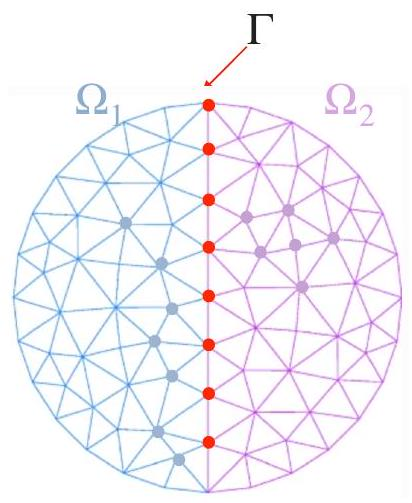
\includegraphics[scale = 0.35]{2023_09_05_b72ccc85584d9dc6fb5cg-191}
\end{center}
Partitioning the matrix and right-hand side vector accordingly, we obtain a symmetric block linear system. 
$$
\left(\begin{array}{ccc}
A_{11} & 0 & A_{1 \Gamma} \\
0 & A_{22} & A_{2 \Gamma} \\
A_{1 \Gamma}^{T} & A_{2 \Gamma}^{T} & A_{\Gamma \Gamma}
\end{array}\right)\left(\begin{array}{l}
\mathbf{x}_{1} \\
\mathbf{x}_{2} \\
\mathbf{x}_{\Gamma}
\end{array}\right)=\left(\begin{array}{l}
\mathbf{b}_{1} \\
\mathbf{b}_{2} \\
\mathbf{b}_{\Gamma}
\end{array}\right)
$$
Zero blocks result from assumption that nodes in $\Omega_{1}$ are not directly connected to nodes in $\Omega_{2}$, but only through interface nodes in $\Gamma$. \\
Block LU factorization of matrix A yields:
$$
\left(\begin{array}{ccc}
A_{11} & 0 & A_{1 \Gamma} \\
0 & A_{22} & A_{2 \Gamma} \\
A_{1 \Gamma}^{T} & A_{2 \Gamma}^{T} & A_{\Gamma \Gamma}
\end{array}\right)=\left(\begin{array}{ccc}
I & 0 & 0 \\
0 & I & 0 \\
A_{1 \Gamma}^{T} & A_{11}^{-1} & I
\end{array}\right)\left(\begin{array}{ccc}
A_{11} & 0 & A_{1 \Gamma} \\
0 & A_{22} & A_{2 \Gamma} \\
0 & 0 & S
\end{array}\right)
$$
where $S$ is the schur complement:
$$
S=A_{\Gamma \Gamma}-A_{1 \Gamma}^{T} A_{11}^{-1} A_{1 \Gamma}-A_{2 \Gamma}^{T} A_{22}^{-1} A_{2 \Gamma}.
$$
We can now determine interface unknowns $\mathbf{u}_{\Gamma}$ by solving system:
$$
S \mathbf{x}_{\Gamma}=\widetilde{\mathbf{b}}_{\Gamma}
$$
where:
$$
\widetilde{\mathbf{b}}_{\Gamma}=\mathbf{b}_{\Gamma}-A_{1 \Gamma}^{T} A_{11}^{-1} \mathbf{b}_{1}-A_{2 \Gamma}^{T} A_{22}^{-1} \mathbf{b}_{2}
$$
The remaining unknowns (which can be computed simultaneously) are then given by:
$$
\begin{aligned}
& \mathbf{x}_{1}=A_{11}^{-1}\left(\mathbf{b}_{1}-A_{1 \Gamma} \mathbf{x}_{\Gamma}\right) \\
& \mathbf{x}_{2}=A_{22}^{-1}\left(\mathbf{b}_{2}-A_{2 \Gamma} \mathbf{x}_{\Gamma}\right)
\end{aligned}
$$

\section*{The schur complement system: remarks}
The Schur complement matrix $S$ is expensive to compute and is generally dense even if $A$ is sparse. If the Schur complement system $S \mathbf{x}_{\Gamma}=\widetilde{\mathbf{b}}_{\Gamma}$ is solved iteratively, then $S$ need not be formed explicitly.
The Schur complement system, denoted as $S \mathbf{x}_{\Gamma}=\widetilde{\mathbf{b}}_{\Gamma}$, is a system of linear equations. Solving this system directly would require forming the matrix $S$, which is computationally expensive, especially if $S$ is a large matrix.
However, if we use iterative methods to solve this system, such as the Conjugate Gradient method or the Gauss-Seidel method, we don't need to form the matrix $S$ explicitly. These iterative methods only require the result of a matrix-vector multiplication at each step.
Matrix-vector multiplication by $S$ requires the solution in each subdomain, implicitly involving $A_{11}^{-1}$ and $A_{22}^{-1}$, which can be done in parallel. The condition number of $S$ is generally better than that of $A$, typically $O\left(h^{-1}\right)$ instead of $O\left(h^{-2}\right)$ for mesh size $h$. In practice, suitable interface pre-conditioners are still needed to accelerate convergence. The term "interface preconditioners" refers to preconditioners that are specifically designed for problems where the domain is divided into subdomains, and the preconditioner operates on the "interface" between these subdomains. 


\section*{Many Non-Overlapping Subdomains}
To improve parallelism with the Schur method, we can use many subdomains. If there are $p$ non-overlapping subdomains, let $I$ be the set of indices of interior nodes of subdomains and, as before, let $\Gamma$ be the set of indices of interface nodes. Then the discrete linear system has the following block form: \\

$$\left(\begin{array}{cc}A_{I I} & A_{I \Gamma} \\A_{I  \Gamma}^{T} & A_{\Gamma \Gamma}\end{array}\right)\left(\begin{array}{l}\mathbf{x}_{I} \\\mathbf{x}_{\Gamma}\end{array}\right)=\left(\begin{array}{l}\mathbf{b}_{I} \\\mathbf{b}_{\Gamma}\end{array}\right)$$ 
The matrix $A_{I I}$ is block diagonal and has the following structure: $$A_{I I}=\left(\begin{array}{cccc}A_{11} & 0 & \ldots & 0 \\0 & A_{22} & \ldots & 0 \\0 & \vdots & \ddots & 0 \\0 & \ldots & 0 & A_{p p}\end{array}\right)$$ As before, block LU factorization of matrix A yields a system:

$$S \mathbf{x}_{\Gamma}=\widetilde{\mathbf{b}}_{\Gamma}$$ where the Schur complement matrix $S$ is given by $$S=A_{\Gamma \Gamma}-A_{I \Gamma}^{T} A_{I I}^{-1} A_{I \Gamma}.$$
This system can be solved again iteratively without forming $S$ explicitly. Suitable interface preconditioners can be used to accelerate convergence. Interior unknowns are then given by:
$$\mathbf{x}_{I}=A_{I I}^{-1}\left(\mathbf{b}_{I}-A_{I \Gamma} \mathbf{x}_{\Gamma}\right).$$
All the occurrences of $A_{I I}^{-1}$ can be performed on all subdomains in parallel because $A_{I I}$ is block diagonal.

\section*{How to evaluate the efficiency of a domain decomposition?}

Weak scalability refers to how the solution time varies with the number of processors for a fixed problem size per processor. It is not achieved with the one-level method. When we say a method doesn’t achieve weak scalability, it means that as we increase the number of processors, the time to solution does not remain constant even though each processor is working on a fixed size of the problem.
In an ideal weakly scalable system, if we double the number of processors and double the size of the problem, the time to solution should remain the same. However, if a method doesn’t achieve weak scalability, then doubling the number of processors and the size of the problem would lead to an increase in the time to solution. Without the coarse correction, the iteration count increases linearly with the number of subdomains. 


\chapter{Direct methods for sparse linear
systems}
\section*{LU factorization}
Let $A_{p, i} \in \mathbb{R}^{i, i}, i=1, \ldots, n$ be the principal sub-matrices of $A$ obtained by considering the first rows and columns
$$
\begin{aligned}
& {\left[\begin{array}{ccc|cc}
a_{11} & \ldots & a_{1 i} & \ldots & a_{1 n} \\
\vdots & & & & \\
a_{i 1} & \ldots & a_{i i} & & \vdots \\
a_{n 1} & \ldots & & \ldots & a_{n n}
\end{array}\right]} \\
& \operatorname{det}\left(A_{p, i}\right) \ \neq 0 \forall i=1, \ldots, n-1
\end{aligned}
$$
\textbf{LU factorization.} Let $A$ be a square matrix. An LU factorization refers to the factorization of $A$ into two factors: a lower unitary triangular matrix $L$ and an upper triangular matrix: $A=LU$.\\ \\
\textbf{Theorem}: If $A$ is invertible, then it admits an LU factorization if and only if all its leading principal minors are nonzero.

\section*{Gaussian elimination}
It consists of a sequence of operations (swapping two rows, multiplying a row by a nonzero number, adding a multiple of one row to another row) performed on the corresponding matrix of coefficients, so as to "transform" $A$ into an upper triangular matrix $\left(A^{(n)}=U\right)$.\\ \\ 
For $k=1, \ldots, n$ \\       
$A^{(1)}=A \rightarrow A^{(2)} \rightarrow \ldots \rightarrow A^{(k)} \rightarrow A^{(k+1)} \rightarrow \ldots \rightarrow A^{(n)}=U$.\\
$\boldsymbol{b}^{(1)}=\boldsymbol{b} \rightarrow \boldsymbol{b}^{(2)} \rightarrow \ldots \rightarrow \boldsymbol{b}^{(k)} \rightarrow \boldsymbol{b}^{(k+1)} \rightarrow \ldots \rightarrow \boldsymbol{b}^{(n)}=\boldsymbol{y}$. \\ \\
To do this in practice, a multiple of row $k$ is subtracted from the subsequent rows in order to cancel the desired elements. \\ \\
For $k=1, \ldots, n-1$\\
\hspace*{1em} For $i=k+1, \ldots, n$\\
\hspace*{2em} $l_{i k}=\frac{a_{i k}^{(k)}}{a_{k k}^{(k)}}$\\
\hspace*{2em} For $j=k+1, \ldots, n$\\
\hspace*{3em} $ a_{i j}^{(k+1)}=a_{i j}^{(k)}-l_{i k} a_{k j}^{(k)} $\\
\hspace*{2em} $b_i^{(k+1)}=b_i^{(k)}-l_{i k} b_k^{(k)}$\\ \\
After $\mathrm{n}$ steps we have:
$A^{(n)}=U$, \ $l_{i j} \rightarrow L$, \ $\boldsymbol{b}^{(n)}=\boldsymbol{y}$.
\subsection*{A practical example}
\textbf{Gaussian Elimination}
$$
A=\left[\begin{array}{ccc}
1 & 1 / 2 & 1 / 3 \\
1 / 2 & 1 / 3 & 1 / 4 \\
1 / 3 & 1 / 4 & 1 / 5
\end{array}\right] \quad \boldsymbol{b}=\left[\begin{array}{c}
11 / 6 \\
13 / 12 \\
47 / 60
\end{array}\right]
$$

$$
\begin{gathered}
\longrightarrow A^{(2)}=\left[\begin{array}{ccc}
1 & 1 / 2 & 1 / 3 \\
0 & 1 / 12 & 1 / 12 \\
0 & 1 / 12 & 4 / 45
\end{array}\right] \quad \boldsymbol{b}^{(2)}=\left[\begin{array}{c}
11 / 6 \\
1 / 6 \\
31 / 180
\end{array}\right] \\
\longrightarrow U=A^{(3)}=\left[\begin{array}{ccc}
1 & 1 / 2 & 1 / 3 \\
0 & 1 / 12 & 1 / 12 \\
0 & 0 & 1 / 180
\end{array}\right] \quad \boldsymbol{y}=\boldsymbol{b}^{(3)}=\left[\begin{array}{c}
11 / 6 \\
1 / 6 \\
1 / 180
\end{array}\right]
\end{gathered}
$$
\textbf{Backward substitution}
$$
\begin{aligned}
x_{3}=\frac{1 / 180}{1 / 180}=1 \longrightarrow x_{2}=\frac{1 / 6-1 / 12 \cdot 1}{1 / 12} & =1 \\
& \longrightarrow x_{1}=\frac{11 / 6-1 / 2 \cdot 1-1 / 3 \cdot 1}{1}=1
\end{aligned}
$$

\subsection*{Gaussian elimination: computational costs}
For any $$k=1, \ldots, n$$
$$
\begin{aligned}
\sum_{k=1}^{n-1}  k+ \left(2(n-k)^{2}+3(n-k)\right)=\sum_{p=1}^{n-1}k+\left(2 p^{2}+3 p\right) & = \\
=k(n-1)+ 2 \frac{n(n-1)(2 n-1)}{6}+3 \frac{n(n-1)}{2} & \sim 2 / 3 n^{3}
\end{aligned}
$$

\subsection*{Sufficient conditions for Gaussian elimination}
\begin{enumerate}
  \item $A$ is strictly diagonally dominant by rows/columns.
  \item  $A$ is SPD.
\end{enumerate}

\section*{Cholesky factorisation (A is SPD)}
Let $A$ be a SPD matrix of order $n$. Then, there exists a unique upper triangular matrix $R$ with real and positive diagonal entries such that: $A=R^{T} R$.\\  \\
Let $r_{11}=\sqrt{a_{11}}$. \\
For $j=2, \ldots, n$
$$
\begin{aligned}
& r_{i j}=\frac{1}{r_{i i}}\left(a_{i j}-\sum_{k=1}^{i-1} r_{k i} r_{k j}\right), i=1, \ldots, j-1 \\
& r_{j j}=\sqrt{a_{j j}-\sum_{k=1}^{j-1} r_{k j}^{2}}
\end{aligned}
$$
Computational cost $\approx n^{3} / 3$


\section*{Pivoting}
\subsection*{Pivoting Techniques}
If at the step $k$ of Gaussian Elimination the pivotal element $a_{k k}^{(k)}=0$ then the algorithm switches row $k$ with row $i>k$, where the index $i$ is chosen so that $a_{i k}^{(k)} \neq 0$.

\subsection*{Pivoting by rows}
As a matter of fact, if at step $k$ row $k$ is swapped with row $i>k$, it is equivalent to pre-multiplying $A^{(k)}$ by a matrix obtained by exchanging the $k$-th and $i$-th rows in the identity matrix:
$$
\begin{aligned}
& A=A^{(1)} \rightarrow P^{(1)} A^{(1)} \rightarrow A^{(2)} \rightarrow P^{(2)} A^{(2)} \rightarrow A^{(3)} \rightarrow \ldots \rightarrow A^{(n)} \\
& P=P^{(n-1)} P^{(n-2)} \ldots P^{(1)}
\end{aligned}
$$
The pivotal element should be as large as possible to "avoid" round-off errors. In practice:
\begin{itemize}
  \item Do pivoting even when it is not strictly needed $\left(a_{k k}^{(k)} \neq 0\right)$.
  \item Swap the row $k$ with the row $\bar{i}$, where $\bar{i}$ is chosen to maximize $\left|a_{i k}^{(k)}\right|$ for $i=k, \ldots, n$.
\end{itemize}

\section*{Complete pivoting}
 Complete pivoting searches for the largest element in magnitude in the entire remaining submatrix, not just in a particular row or column, and then swaps rows and columns to place that value in the upper left position. This is equivalent to introducing a second permutation matrix $Q$:
$$
PA Q=LU.
$$
$$
\mathrm{Ax}=\mathrm{b} \Leftrightarrow \underbrace{\mathrm{PAQ}}_{\mathrm{LU}} \underbrace{\mathrm{Q}^{-1} \mathrm{x}}_{\mathrm{x}^{*}}=\mathrm{Pb} \Longrightarrow \mathrm{Ly}=\mathrm{Pb} \quad \mathrm{Ux}^{*}=\mathbf{y} \quad \mathrm{x}=\mathrm{Qx}^{*}
$$

\subsection*{Fill-in}
When $A$ is sparse, $\mathrm{LU}$ decomposition results in $\mathrm{L}, \mathrm{U}$ with non-zeros (called fill-in) at positions that were originally zero.\\
Gaussian Elimination (in its plain version) is made in such a way as to memorise $L$ and $U$ by overwriting the space allocated for $A$.\\
LU factorisation is not suitable from the point of view of memory occupation for sparse matrices.

\section*{Fill-in reduction strategies}
To reduce fill-in, it may be useful to employ reordering techniques, which consists in numbering the rows of A differently. The aim is to reduce the number of non-zeros in $L, U$ by permuting the nonzero structure of $A$ into a special form and respecting this form when performing the reordering.

\section*{Sparse direct methods}
The sequence in which variables are arranged can significantly impact the efficiency of numerical computations. This influence stems from variable ordering affecting several critical aspects, including the elimination tree, parallelism, computation, and memory usage.  \\
The elimination tree, a data structure representing the nonzero structure of a matrix used in sparse matrix factorization, plays a pivotal role. It aids in estimating storage and computational requirements, ascertaining dependencies between columns, facilitating parallel processing, and enabling advanced sparsification techniques.  \\
Hence, dedicating time to matrix analysis before embarking on factorization proves advantageous. However, it's vital to recognize that determining the optimal ordering to minimize fill-in (the introduction of new non-zero elements in factored matrices) is a challenging NP-hard problem, lacking an efficient solution algorithm. Nonetheless, heuristics can be deployed to investigate and optimize tree topology, including node count and sizes.  \\
To solve a system of linear equations represented as $A\mathbf{x}=\mathbf{b}$, three primary phases are involved:  
\begin{enumerate}  
\item Analysis of matrix $A$ (symbolic phase): This phase encompasses identifying suitable permutation matrices $P$ and $Q$ based on $A$'s nonzero structure to minimize fill-in. It entails computing the elimination tree and preparing for parallel execution by mapping tree nodes to different processors. Each processor then configures its local data structures accordingly.  
\item Factorization of $A$ (numerical factorization): The factors are determined using the elimination tree. It may be necessary to post-process (a-posteriori) modify $P$ and $Q$ to ensure numerical stability. Numerical stability pertains to the factorization process's sensitivity to small changes in the input matrix or to round-off errors during computation.  
\item Forward/backward substitution: In this phase, we solve for $x$ given $b$, utilizing the factors obtained in phase 2.  
\end{enumerate}  
  


\section*{The symbolic phase (idea)}
The symbolic phase is an integral part of matrix factorization. 
The symbolic phase typically involves two main steps:  
\begin{enumerate}  
\item Finding a good fill-reducing permutation. This involves identifying a permutation of the matrix's rows and columns that minimizes the number of non-zero elements that are introduced during factorization (known as "fill-in"). Minimizing fill-in can significantly reduce the computational and memory requirements of the factorization process.  
\item Once the ordering is found, the symbolic phase proceeds to determine the elimination tree and the nonzero pattern of the factorization. In addition, it identifies key properties such as the number of nonzeros in each row and column of the factors. These insights can further optimize the factorization process and are crucial for understanding the structure of the matrix.  
\end{enumerate}    
The symbolic phase is less problematic compared to the numerical factorization phase. For one, it is asymptotically faster. This means that as the problem size increases, the time taken by the symbolic phase grows at a slower rate compared to the numerical phase. Furthermore, the symbolic phase enables the numerical phase to be more efficient in terms of time and memory. By determining the structure and sparsity pattern of the matrix in advance, the symbolic phase allows for more optimized computations during the numerical phase. Another significant advantage of the symbolic phase is that it allows for the numeric factorization to be repeated for a sequence of matrices with an identical nonzero pattern. This feature is particularly useful when solving non-linear and/or differential equations, where the structure of the matrix remains the same, but the actual values might change.  



\section*{Fill-in reducing orderings}
\subsection*{The fill-in minimization problem}
The fill-in minimization problem can be stated as follows:\\ \\
Given a matrix $A$, find a row and column permutation $P$ and $Q$ (with the added constraint that $Q=P^{T}$ for a sparse Cholesky factorization) such that the number of non-zeros in the factorization of $PAQ$ (or the amount of work required to compute it) are minimized.\\ \\
Computing an ordering for the minimum fill is NP-hard, in its many forms. The primary aim is to minimize the number of non-zero elements in the factorization, also known as fill-in. This is because sparse matrices, which have many zero elements, can be stored and manipulated more efficiently than dense matrices. By minimizing fill-in, we maintain sparsity and thus save on storage and computational resources.\\
Moreover, minimizing fill-in often also leads to a reduction in the computational work required for the factorization. This is because operations with zero elements do not need to be performed, so fewer non-zero elements means fewer operations. Therefore, while the primary aim is to minimize fill-in, this often also results in a reduction in the time to compute the factorization. So, both aspects are interconnected. There are many approaches to tackle this problem:

\begin{enumerate}  
    \item \textbf{Symmetric minimum degree:} This is a heuristic widely used for finding a permutation $P$ such that $P A P^{T}$ has fewer non-zeros in its factorization than $A$. It is a greedy method that selects the pivot row and column with the fewest non-zero elements during the course of a right-looking sparse Cholesky factorization.  
      
    \item \textbf{Unsymmetric minimum degree:} This method is similar to symmetric minimum degree but it does not require the matrix to be symmetric. It is used when the matrix $A$ is not symmetric and we cannot apply symmetric minimum degree.  
      
    \item \textbf{Nested dissection:}  Consider the undirected graph of a matrix $A$ with symmetric nonzero pattern. Nested dissection finds a vertex separator that splits the graph into two or more roughly equal-sized subgraphs (left and right), when the vertices in the separator (and their incident edges) are removed from the graph. The subgraphs are then ordered recursively, which helps in reducing fill-in during factorization.  It can be applied only to symmetric matrices. 
      
    \item \textbf{Permutations to block-triangular-form, and other special forms:} This approach involves permuting rows and columns of a matrix to bring it into a block triangular form or other special forms which can simplify computations or reduce fill-in during factorization.   
\end{enumerate}  


\section*{Sparse matrices and graphs}
\subsection*{Symmetric sparse matrices and graphs}
The structure of a square symmetric matrix $A$ with nonzero diagonal can be represented by an undirected graph $G(A)=(V, E)$ with:
\begin{itemize}
  \item $n$ vertices, one for each row/column of $A$;

  \item an edge $(\mathrm{i}, \mathrm{j})$ for each nonzero $a_{i j}, i>j$.

\end{itemize} 
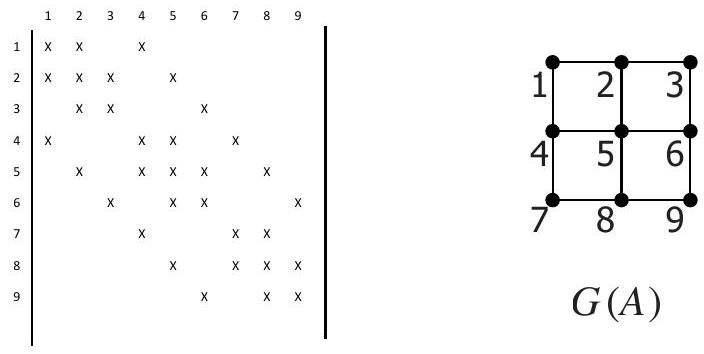
\includegraphics[scale = 0.4, center]{2023_09_05_b72ccc85584d9dc6fb5cg-225}

\section*{Non-symmetric sparse matrices and graphs}
The structure of a non-symmetric matrix of size $n \times n$ can be represented by:
\begin{itemize}
    \item A directed graph $G(A) = (V, E)$ with
    \begin{itemize}
        \item $n$ vertices, one for each column of $A$.
        \item an edge from $i$ to $j$ for each nonzero $a_{ij}$.
    \end{itemize}
    \item A bipartite graph $H(A) = (V, E)$ with
    \begin{itemize}
        \item $2n$ vertices, for rows and columns of $A$
        \item an edge $(i', j)$ for each nonzero $a_{ij}$.
    \end{itemize}
\end{itemize}

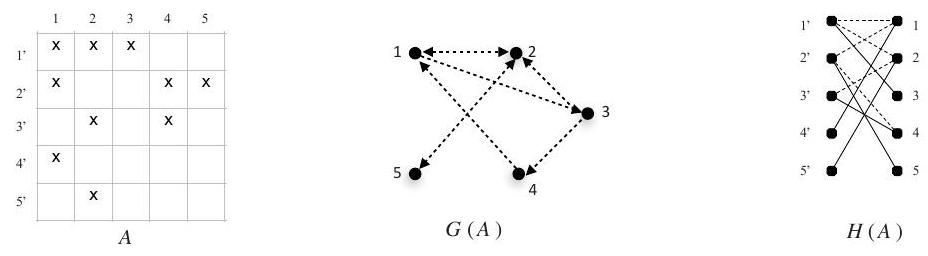
\includegraphics[scale = 0.4, center]{2023_09_05_b72ccc85584d9dc6fb5cg-226}

\subsection*{Filled graph $G^{+}(A)$, A SPD}

Given $G(A)=(V, E)$, $G^{+}(A)=\left(V, E^{+}\right)$ is defined as follows: there is an edge $(i, j) \in G^{+}(A)$ if and only if there is a path from $i$ to $j$ in $G(A)$ going through lower numbered vertices. The same definition holds also for directed graphs.\\ \\ 
\textbf{Useful remark}: $G\left(R+R^T\right)=G^{+}(A)$ (ignoring cancellations). "Ignoring cancellations" means that when constructing the graph $G\left(R+R^T\right)$, we do not consider the possibility that some elements in $R+R^T$ might cancel each other out and result in a zero entry. \\
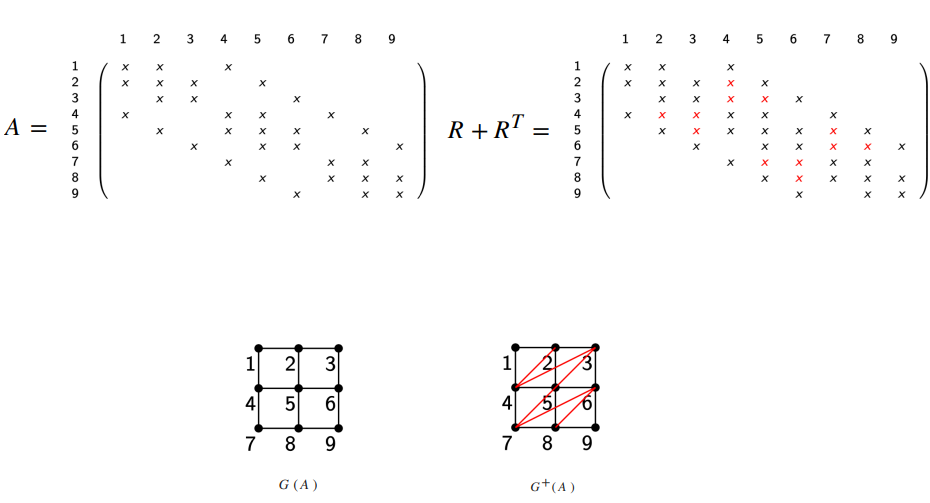
\includegraphics[max width=\textwidth, center]{images/Screen0.png}


\subsection*{Filled graph $G^{+}(A)$, A non-symmetric}

A is square, non-symmetric (nonzero diagonal entries). The nonzero structure of $L$ and $U$ can be determined prior to the numerical factorisation from the structure of $A$.\\
Filled graph:
\begin{itemize}
    \item Edges from rows to columns for all non-zeros of $A$.
    \item Add fill edge if there is a path from $i$ to $j$ in $G(A)$ through lower numbered vertices.
\end{itemize}
\textbf{Remark}: $G\left(R+R^T\right)=G^{+}(A)$ (ignoring cancellations).\\
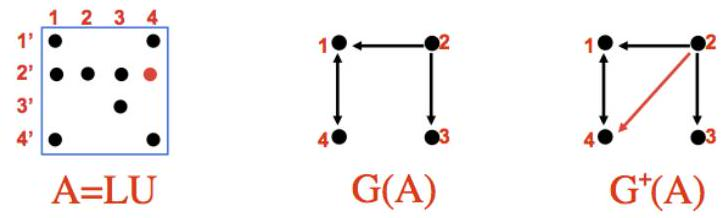
\includegraphics[max width=\textwidth, center]{2023_09_05_b72ccc85584d9dc6fb5cg-229}



\section*{Steps of sparse Cholesky factorisation}
\begin{enumerate}
    \item Order rows and columns of to reduce fill-in.
    \item Symbolic factorization (based on eliminaton trees).
    \begin{itemize}
        \item Compute the elimination tree.
        \item Allocate data structure. 
        \item Compute the nonzero structure of the factor R.
    \end{itemize}
    \item Factorization. 
    \item Triangular solve.
\end{enumerate}

\section*{Multifrontal direct methods}
The multifrontal method is a technique used to simplify the factorization of sparse matrices. It does this by breaking down the overall factorization into a series of smaller, dense submatrix factorizations. 
This process is guided by an elimination tree, which is a graphical representation of the dependencies between these partial factorizations. The structure of the matrix and the ordering of the variables (also known as permutations) determine this tree.
Here's a more detailed explanation:
\begin{itemize}
\item  Each node in the tree represents a partial factorization of a small, dense matrix.
\item  Each edge in the tree signifies the transfer of data between these dense matrices.
\item The tree establishes a partial order: a node can only be processed once all its child nodes have been processed. This means that the leaves (the nodes without any children) are processed first, while the root (the topmost node) is processed last.
\item Nodes that do not have an ancestor-descendant relationship can be processed at the same time, allowing for parallel processing.
\end{itemize}
In simpler terms, this method organizes the complex task of matrix factorization into manageable parts, following a specific order dictated by an elimination tree. This not only makes the process more efficient but also opens up opportunities for parallel computation.\\ \\
See Slides Pack n. 6 Pages 36-51 for visualization.

\section*{Examples of direct solvers}
An incomplete list of solvers and their characteristics:

\begin{itemize}
  \item PSPASES: for SPD matrices, distributed memory.

  \item UMFPACK / SuiteSparse (Matlab, Google Ceres) - symmetric/nonsymmetric, LU, QR, multicores/GPUs.

  \item SuperLU: non-symmetric matrices, shared/distributed memory.

  \item MUMPS: symmetric/non-symmetric, distributed memory.

  \item Pardiso (Intel MKL): symmetric/unsymmetric, shared/distributed memory.

\end{itemize}

\newpage 
\chapter{Eigenvalue problems}
The algebraic eigenvalue problem reads as follows:\\
Given a matrix $A \in \mathbb{C}^{n \times n}$, find $(\lambda, \mathbf{x}) \in \mathbb{C} \times \mathbb{C}^{n} \backslash\{\mathbf{0}\}$ such that:
$$
A \mathbf{v}=\lambda \mathbf{v}
$$
where $\lambda$ is an eigenvalue of $A$ and $\mathbf{v}$ (non-zero) is the corresponding eigenvector.
The set of all the eigenvalues of a matrix $\mathrm{A}$ is called the spectrum of $\mathrm{A}.$
The module of the eigenvalue with the maximum one is called the spectral radius of $A$:
$$
\rho(A)=\max \{|\lambda|: \lambda \in \lambda(A)\}
$$

\section*{Geometric interpretation}
Eigenvalues and eigenvectors provide a means of understanding the complicated behavior of a general linear transformation by decomposing it into simpler actions.\\
An eigenvector (corresponding to a real nonzero eigenvalue) points in a direction in which it is stretched by the linear transformation; the associated eigenvalue is the factor by which it is "stretched/contracted".

\section*{Mathematical background}
\begin{enumerate}
  \item The problem $A \mathbf{v}=\lambda \mathbf{v}$ is equivalent to $(A-\lambda I) \mathbf{v}=0$.

  \item This homogeneous equation has a nonzero solution $\mathbf{v}$ if and only if its matrix is singular. The eigenvalues of $A$ are the values $\lambda$ such that $\operatorname{det}(A-\lambda I)=0$.

  \item $\operatorname{det}(A-\lambda I)=0$ is a polynomial of degree $n$ in $\lambda$ : it is called the characteristic polynomial of $A$ and its roots are the eigenvalues of $A$.

\end{enumerate}

\section*{Some useful remarks}
\begin{itemize}
  \item From the Fundamental Theorem of Algebra, an $n \times n$ matrix $A$ always has $n$ eigenvalues $\lambda_{i}, \ i=1, \ldots, n$.

  \item Each $\lambda_{i}$ may be real but in general is a complex number.

  \item The eigenvalues $\lambda_{1}, \lambda_{2}, \ldots, \lambda_{n}$ may not all have distinct values.

  \item Rayleigh quotient: Let $\left(\lambda_{i}, \mathbf{v}_{i}\right)$ be an eigenpair of $A$, then:
$$
\lambda_{i}=\frac{\mathbf{v}_{i}^{H} A \mathbf{v}_{i}}{\mathbf{v}_{i}^{H} \mathbf{v}_{i}}
$$
The exponent $^H$ indicates the conjugate transpose of a vector.

\end{itemize}
We first need to identify:
\begin{itemize}
  \item What types of transformations preserve eigenvalues;

  \item For what types of matrices the eigenvalues are easily determined.

\end{itemize}
\textbf{Definition}: The matrix $B$ is similar to the matrix $A$ if there exists a nonsingular matrix $T$ such that $B=T^{-1} A T$.
With the above definition, it is trivial to show that:
$$
B \mathbf{y}=\lambda \mathbf{y} \rightarrow T^{-1}AT \mathbf{y}=\lambda \mathbf{y} \rightarrow A(T\mathbf{y})=\lambda(T \mathbf{y})
$$
so that $A$ and $B$ have the same eigenvalues, and if $\mathbf{y}$ is an eigenvector of $B$, then $\mathbf{v}=T \mathbf{y}$ is an eigenvector of $A$ \\ \\
\textbf{Similarity transformations} preserve eigenvalues but do not preserve eigenvectors (but the eigenvectors can be easily recovered).
Note that the converse is not true: two matrices that have the same eigenvalues are not necessarily similar.\\
The eigenvalues of a diagonal matrix are its diagonal entries. The eigenvalues of a triangular matrix are also the diagonal entries. \\
Note that:
\begin{itemize}
  \item Diagonal form simplifies eigenvalue problems for general matrices by similarity transformations.

  \item Some matrices cannot be transformed into diagonal form by a similarity transformation.

\end{itemize}
A square matrix $A$ is called diagonalisable (or non-defective) if it is similar to a diagonal matrix.

\section*{The general idea from the numerical viewpoint}

Some of numerical methods for computing eigenvalues and eigenvectors are based on reducing the original matrix to a simpler form, whose eigenvalues and eigenvectors can  easily be determined.\\
Ideally we would like to transform the underlying system of equations into a special set of coordinate axes in which the matrix is diagonal. The eigenvalues are therefore entries of the diagonal matrix and the eigenvectors are the new set of coordinate axes.

\section*{Computing eigenvalues and eigenvectors}
There are several methods designed to compute all of the eigenvalues of a matrix (and some of them require a great deal of work).
In practice, one may need only one or a few eigenvalues and the corresponding eigenvectors.
The simplest method for computing a single eigenvalue and eigenvector of a matrix is the so called power method.

\section*{Power method}
Assume that the matrix $A$ has a unique eigenvalue $\lambda_{1}$ of maximum absolute value, i.e.

$$
\left|\lambda_{1}\right|>\left|\lambda_{2}\right| \geq\left|\lambda_{3}\right| \geq \ldots\left|\lambda_{n}\right|
$$
with the corresponding unitary eigenvector $\mathbf{v}_{1}$.
Starting from a given nonzero vector $\mathbf{x}^{(0)}$, such that $\left\|\mathbf{x}^{(0)}\right\|=1$, let us consider the following iteration scheme, for $k \geq 0$ :
$$
\begin{aligned}
\mathbf{y}^{(k+1)} & \leftarrow A \mathbf{x}^{(k)} \\
\mathbf{x}^{(k+1)} & \leftarrow \frac{\mathbf{y}^{(k+1)}}{\left\|\mathbf{y}^{(k+1)}\right\|} \\
\nu^{(k+1)} & \leftarrow\left[\mathbf{x}^{(k+1)}\right]^{H} A \mathbf{x}^{(k+1)}
\end{aligned}
$$
It can be shown that the above iteration scheme converges to a multiple $\mathbf{v}_{1}$, the eigenvector corresponding to the dominant eigenvalue $\lambda_{1}$.

\subsection*{Hints of the Proof}
\begin{enumerate}
    \item Observe that since $A$ is diagonalisable, its eigenvector $\mathbf{v}_{i}$ forms a basis for $\mathbb{C}^{n}$.
    \item Express the starting vector $\mathbf{x}^{(0)}$ as a linear combination of the eigenvectors.
    \item Do some calculations to obtain:
           $$y^{k} = A^{k} x^{(0)}=\alpha_{1} \lambda_{1}^{k}\left(\mathbf{v}_{\mathbf{1}}+\sum_{i=2}^{n} \frac{\alpha_{i}}{\alpha_{1}}\left[\frac{\lambda_{i}}{\lambda_{1}}\right]^{k} \mathbf{v}_{\mathbf{i}}\right).$$
    \item The term $\lambda_{1}$ is the dominant eigenvalue, meaning its absolute value is larger than the absolute values of all other eigenvalues. Because of this, as $k$ increases, the terms involving $\frac{\lambda_{i}}{\lambda_{1}}$ for $i>1$ will tend to zero (since $|\frac{\lambda_{i}}{\lambda_{1}}|<1$), and the iteration will converge to a multiple of $\mathbf{v}_{1}$, the eigenvector corresponding to the dominant eigenvalue.
\end{enumerate}
\section*{Convergence rate of the power method}
The convergence rate of the power method depends on the ratio $\left|\lambda_{2}\right| /\left|\lambda_{1}\right|$, where $\lambda_{2}$ is the eigenvalue having the second largest absolute value.
The smaller $\left|\lambda_{2}\right| /\left|\lambda_{1}\right|$ is, the faster the convergence is.\\
Hence the power method will converge quickly if $\left|\lambda_{2}\right| /\left|\lambda_{1}\right|$ is small and slowly if $\left|\lambda_{2}\right| /\left|\lambda_{1}\right|$ is close to 1.\\ \\
\textbf{Theorem}. Suppose $\left|\lambda_1\right|>\left|\lambda_2\right| \geq \cdots \geq\left|\lambda_m\right| \geq 0$ and $\mathbf{v}_1^T \mathbf{x}^{(0)} \neq 0$. Then the iterates of the Power Method satisfy:
$$
\left\|\mathbf{x}^{(k)}-\left( \pm \mathbf{v}_1\right)\right\|=O\left(\left|\frac{\lambda_2}{\lambda_1}\right|^k\right), \quad\left|\lambda^{(k)}-\lambda_1\right|=O\left(\left|\frac{\lambda_2}{\lambda_1}\right|^{2 k}\right)
$$
as $k \rightarrow \infty$. The $\pm$ sign means that at each step $k$, one or the other choice of sign is to be taken, and then the indicated bound holds.
The reference for this theorem is Theorem 27.1 from the Numerical Linear Algebra Book by Trefethen.

\section*{Deflation method}

The elementary Householder tranformations can be conveniently employed to compute the first (largest or smallest) eigenvalues of a given matrix $A \in \mathbb{R}^{n \times n}$. Assume that the eigenvalues of A are ordered as previously stated and suppose that the eigenvalue/eigenvector pair $\left(\lambda_1, \mathbf{x}_1\right)$ has been computed using the power method. Then the matrix A can be transformed into the following block form:
$$
\mathrm{A}_1=\mathrm{HAH}=\left(\begin{array}{ll}
\lambda_1 & \mathbf{b}^T \\
0 & \mathrm{~A}_2
\end{array}\right)
$$
where $\mathbf{b} \in \mathbb{R}^{n-1}, \mathrm{H}$ is the Householder matrix such that $\mathrm{Hx}_1=\alpha \mathbf{x}_1$ for some $\alpha \in \mathbb{R}$, the matrix $\mathrm{A}_2 \in \mathbb{R}^{(n-1) \times(n-1)}$ and the eigenvalues of $\mathrm{A}_2$ are the same as those of $\mathrm{A}$ except for $\lambda_1$. The matrix $\mathrm{H}$ can be computed using with $\mathbf{v}=\mathbf{x}_1 \pm\left\|\mathbf{x}_1\right\|_2 \mathbf{e}_1$.

The deflation procedure consists of computing the second dominant (subdominant) eigenvalue of $\mathrm{A}$ by applying the power method to $\mathrm{A}_2$ provided that $\left|\lambda_2\right| \neq\left|\lambda_3\right|$. Once $\lambda_2$ is available, the corresponding eigenvector $\mathbf{x}_2$ can be computed by applying the inverse power iteration to the matrix $\mathrm{A}$ taking $\mu=\lambda_2$  and proceeding in the same manner with the remaining eigenvalue/eigenvector pairs. 

\section*{Inverse power method}
For some applications, the smallest eigenvalue of a matrix is required rather than the largest. We use the fact that the eigenvalues of $A^{-1}$ are the reciprocals of those of $A$.
Hence the smallest eigenvalue of $A$ is the reciprocal of the largest eigenvalue of $A^{-1}$.\\ \\
Starting from a given nonzero vector $\mathbf{q}^{(0)}$, such that $\left\|\mathbf{q}^{(0)}\right\|=1$, let us consider the following iteration scheme, for $k \geq 0$ :

\begin{enumerate}
\item Solve $A \mathbf{z}^{(k+1)}=\mathbf{q}^{(k)}$
\item $\mathbf{q}^{(k+1)} \leftarrow \frac{\mathbf{z}^{(k+1)}}{\left\|\mathbf{z}^{(k+1)}\right\|}$
\item $\sigma^{(k+1)} \leftarrow\left[\mathbf{q}^{(k+1)}\right]^{H} A \mathbf{q}^{(k+1)}$
\end{enumerate}
In the standard power method, we start with an initial guess for the eigenvector and multiply it by the matrix in each iteration. This process is repeated until the sequence converges to the dominant eigenvector (the one corresponding to the largest eigenvalue in absolute value). The corresponding eigenvalue can then be computed using the Rayleigh quotient.\\ \\
In this method instead of multiplying by the matrix $A$, we are solving a system of linear equations $A \mathbf{z}^{(k+1)}=\mathbf{q}^{(k)}$ at each step. This is equivalent to multiplying by the inverse of the matrix, $A^{-1}$, which effectively flips the spectrum of eigenvalues. As a result, this method converges to the eigenvector corresponding to the smallest eigenvalue of $A$, rather than the largest.

\section*{Inverse power method with shift}
For any $\mu \in \mathbb{R}$ that is not an eigenvalue of $A$, the eigenvectors of $(A-\mu I)^{-1}$ are the same as the eigenvectors of $A$, and the corresponding eigenvalues are $\left\{\left(\lambda_j-\mu\right)^{-1}\right\}$, where $\left\{\lambda_j\right\}$ are the eigenvalues of $A$. This suggests an idea. Suppose $\mu$ is close to an eigenvalue $\lambda_J$ of $A$. Then $\left(\lambda_J-\mu\right)^{-1}$ may be much larger than $\left(\lambda_j-\mu\right)^{-1}$ for all $j \neq J$. Thus, if we apply power iteration to $(A-\mu I)^{-1}$, the process will converge rapidly to $\mathbf{q}_J$, this is easy to understand remembering the definition of the convergence rate. This idea is called inverse iteration.\\ \\
If we want to approximate the eigenvalue $\lambda$ of $A$ which is the closest to a given number $\mu \notin \sigma(A)$.
We define $M_{\mu}=A-\mu I$ and observe that the eigenvalue $\lambda$ of $A$ which is the closest to $\mu$ is the minimum eigenvalue of $M_{\mu}$.
Starting from a given nonzero vector $\mathbf{q}^{(0)}$, such that $\left\|\mathbf{q}^{(0)}\right\|=1$, let us consider the following iteration scheme, for $k \geq 0$ :

\begin{enumerate} 
\item \begin{tabular}[t]{c} Solve $M_{\mu} \mathbf{z}^{(k+1)}=\mathbf{q}^{(k)}$ \end{tabular}
\item \begin{tabular}[t]{c} $\mathbf{q}^{(k+1)} \leftarrow \frac{\mathbf{z}^{(k+1)}}{\left\|\mathbf{z}^{(k+1)}\right\|}$ \end{tabular}
\item \begin{tabular}[t]{c} $\nu^{(k+1)} \leftarrow\left[\mathbf{q}^{(k+1)}\right]^{H} A \mathbf{q}^{(k+1)}$ \end{tabular}
\end{enumerate}




\section*{QR Factorization $(A=Q R)$}
\section*{Projectors and complementary projectors}
\begin{itemize}
  \item A projector is a square matrix $P \in \mathbb{R}^{n \times n}$ that satisfies $P = P^{2}$.

  \item If $\mathbf{w} \in \operatorname{range}(P)$, then $P \mathbf{w}=\mathbf{w}$. Indeed, since $\mathbf{w} \in \operatorname{range}(P)$, then $\mathbf{w}=P \mathbf{z}$, for some $\mathbf{z}$. Therefore:
$$P \mathbf{w}=P(P \mathbf{z})=P^{2} \mathbf{z}=P \mathbf{z}=\mathbf{w}.$$

  \item The matrix $I-P$ is the complementary projector to $P$.

  \item $I-P$ projects on the nullspace of $P$ : if $P \mathbf{w}=0$, then $(I-P) \mathbf{w}=\mathbf{w}$, so $\operatorname{null}(P) \subseteq \operatorname{range}(I-P)$.

  \item For any $\mathbf{w},(I-P) \mathbf{w}=\mathbf{w}-P \mathbf{w} \in \operatorname{null}(P)$, so range $(I-P) \subseteq \operatorname{null}(P)$.

  \item Therefore:
\begin{itemize}

\item$\operatorname{range}(I-P)=\operatorname{null}(P)$.

\item $\operatorname{null}(I-P)=\operatorname{range}(P)$.
\end{itemize}
\end{itemize}

\section*{Orthogonal Projectors}
A projector $P$ is orthogonal if $P=P^{2}=P^{T}$. We find orthonormal vectors $\left[\mathbf{q}_{1}, \mathbf{q}_{2}, \ldots, \mathbf{q}_{n}\right]$ that span the successive spaces spanned by the columns of $A=\left[\mathbf{a}_{1}, \mathbf{a}_{2}, \ldots, \mathbf{a}_{n}\right]$. This means that for full $\operatorname{rank} A$, $<\mathbf{a}_{1}, \mathbf{a}_{2}, \ldots, \mathbf{a}_{j}>=<\mathbf{q}_{1}, \mathbf{q}_{2}, \ldots, \mathbf{q}_{j}>$ for all $j=1, \ldots, n$.\\
In matrix form, this becomes:
$$\left[\mathbf{a}_1\left|\mathbf{a}_2\right| \cdots \mid \mathbf{a}_n\right]=\left[\mathbf{q}_1\left|\mathbf{q}_2\right| \cdots \mid \mathbf{q}_n\right]\left[\begin{array}{cccc}r_{11} & r_{12} & \ldots & r_{1 n} \\ 0 & r_{22} & \ldots & \vdots \\ 0 & 0 & \ddots & r_{n n}\end{array}\right]$$
This is called the reduced QR factorization.


\section*{The Full QR Factorization}
Let $A$ be an $m \times n$ matrix. The full QR factorization of $A$ is the factorization $A=Q R$, where $Q$ is $m \times m$ orthogonal $\left(Q Q^{T}=I\right)$ and $R$ is $m \times n$ upper-trapezoidal.\\
Similarly, the reduced QR factorization of $A$ is the factorization $A=\hat{Q} \hat{R}$, where $\hat{Q}$ is $m \times n$ and $\hat{R}$ is $n \times n$ upper-triangular. \\
Please note that in both cases, the factorization involves an orthogonal matrix and an upper-triangular (or upper-trapezoidal) matrix. The difference lies in the dimensions of these matrices in the full and reduced QR factorization.

\section*{Gram-Schmidt orthogonalisation}
\begin{itemize}

\item Given $\mathbf{a}_{1}, \mathbf{a}_{2}, \ldots, \mathbf{a}_{n}$ (the columns of $A$), we find a new $\mathbf{q}_{j}$ (the $j$-th column of $\hat{Q}$) orthogonal to $\mathbf{q}_{1}, \ldots, \mathbf{q}_{j-1}$ by subtracting components along previous vectors:

$$
\mathbf{w}_{j}=\mathbf{a}_{j}-\sum_{k=1}^{j-1}\left(\overline{\mathbf{q}}_{k}^{T} \mathbf{a}_{k}\right) \mathbf{q}_{k}
$$
\item We normalize to get $\mathbf{q}_{j}=\frac{\mathbf{w}_{j}}{\left\|\mathbf{w}_{j}\right\|}$.
\item We then obtain a reduced QR factorization $A=\hat{Q}\hat{R}$, with:
$$
r_{i j}=\overline{\mathbf{q}}_{i}^{T} \mathbf{a}_{j} \ \ i \neq j
$$
$$
r_{j j}=|| w_j||
$$
\end{itemize}
Please note that this method can be numerically unstable, which is why the Modified Gram-Schmidt process is often used. Here $\overline{\textbf{q}}_i^{t} = \textbf{q}_i^{H}$.


\section*{Existence and uniqueness}

\textbf{Theorem.} Every $A \in \mathbb{C}^{m \times n}(m \geq n)$ has a full $Q R$ factorization, hence also a reduced $Q R$ factorization.\\ \\
\textbf{Theorem.} Each $A \in \mathbf{C}^{m \times n}$ ( $m \geq n$ ) of full rank has a unique reduced QR factorization $A=\hat{Q} \hat{R}$ with $r_{j j}>0$.\\ \\
The complete proof of these statements can be found in the Book NLA by Trefethen as theorems $7.1$ and $7.2$.\\ \\
By slightly modifying the classical Gram-Schmidt process, we can obtain a modified Gram-Schmidt process. This modified process is numerically stable and less sensitive to rounding errors, which makes it more reliable for computations.
The algorithm for modified G-S is as follows:\\
$$
\begin{aligned}
& \text {for } j=1, \ldots, n \\
& \hspace{1em} \mathbf{w}_{j}=\mathbf{a}_{j} \\
& \hspace{1em} \text { for } i=1, \ldots, j-1 \\
& \hspace{3em} r_{i j}=\overline{\mathbf{q}}_i^T \mathbf{a}_j \\
&  \hspace{3em} r_{i j}=\overline{\mathbf{q}}_{i}^{T} \mathbf{w}_{j} \\
& \hspace{2em} \mathbf{w}_{j}=\mathbf{w}_{j}-r_{i j} \mathbf{q}_{i} \\
& \hspace{2em} r_{j j}=\left\|\mathbf{w}_{j}\right\| \\
& \hspace{2em} \mathbf{q}_{j}=\frac{\mathbf{w}_{j}}{\left\|\mathbf{w}_{j}\right\|} \\
& \hspace{1em} \text { end } \\
& \text { end }
\end{aligned}
$$
The FLOP (Floating Point Operations) count for the MGS process is approximately $2mn^2$, where $m$ is the number of rows and $n$ is the number of columns in the matrix being factorized. It does not distinguish between real and complex numbers, and it does not consider memory accesses or other performance aspects. 

\section*{Schur Decomposition}
If $A \in \mathbb{C}^{n \times n}$, then there exists a unitary matrix $U \in \mathbb{C}^{n \times n}$ such that $U^H AU = T$, where $T$ is upper triangular. The diagonal elements of $T$ are the eigenvalues of $A$. The columns of $U$, denoted as $[u_1, u_2, \ldots, u_n]$, are called Schur vectors. They are generally not eigenvectors.
\section*{Schur Vectors}
The $k$-th column of $U^H AU = T$ reads as $A u_k = \lambda_k u_k + \sum_{i=1}^{k-1} t_{ik} u_i$. This implies that $A u_k \in \text{span} \{u_1, \ldots, u_k\}$ for all $k$. The first Schur vector is an eigenvector of $A$. The first $k$ Schur vectors form an invariant subspace for $A$. The Schur decomposition is not unique.

\section*{Basic QR algorithm}
Let $A \in \mathbb{C}^{n \times n}$. The QR algorithm computes an upper triangular matrix $T$ and a unitary matrix $U$ such that $A=U T U^{H}$ is the Schur decomposition of $A$.
\begin{enumerate}
  \item Set $A^{(0)}=A, U^{(0)}=I$

  \item while(STOPPING CRITERIA)

  \item $A^{(k-1)}=Q^{(k)} R^{(k)}$ (QR factorisation of $A^{(k-1)}$ )

  \item $A^{(k)}=R^{(k)} Q^{(k)}$

  \item $U^{(k)}=U^{(k-1)} Q^{(k)}$ (Update transformation matrix)

  \item end for

  \item $\operatorname{Return} T=A^{(k)}, U=U^{(k)}$.

\end{enumerate}

\section*{Basic QR algorithm: remarks I}
\begin{enumerate}
  \item Notice that $A^{(k)}=R^{(k)} Q^{(k)}=\left[Q^{(k)}\right]^{H} A^{(k-1)} Q^{(k)}$, and therefore $A^{(k)}$ and $A^{(k-1)}$ are similar. Note that the matrix $Q$ is a unitary matrix.

  \item Moreover, from the above observation, we have:

\end{enumerate}

$$
\begin{aligned}
A^{(k)} & =\left[Q^{(k)}\right]^{H} A^{(k-1)} Q^{(k)}= \\
& =\left[Q^{(k)}\right]^{H}\left[Q^{(k-1)}\right]^{H} A^{(k-2)} Q^{(k-1)} Q^{(k)}= \\
& =\ldots= \\
& =\left[Q^{(k)}\right]^{H} \ldots\left[Q^{(1)}\right]^{H} A^{(0)} Q^{(1)} \ldots Q^{(k)}
\end{aligned}
$$

\section*{Convergence of QR method}
Let $\mathrm{A} \in \mathbb{R}^{n \times n}$ be a matrix such that
$$
\left|\lambda_1\right|>\left|\lambda_2\right|>\ldots>\left|\lambda_n\right| \text {. }
$$
Then:
$$
\lim _{k \rightarrow+\infty} \mathrm{A}^{(k)}=\left[\begin{array}{cccc}
\lambda_1 & t_{12} & \ldots & t_{1 n} \\
0 & \lambda_2 & t_{23} & \ldots \\
\vdots & \vdots & \ddots & \vdots \\
0 & 0 & \ldots & \lambda_n
\end{array}\right] .
$$
As for the convergence rate, we have:
$$
\left|a_{i, j}^{(k)}\right|=\mathcal{O}\left(\left|\frac{\lambda_i}{\lambda_{j}}\right|^k\right), \quad \text{for} \ i>k .
$$
Under the additional assumption that $\mathrm{A}$ is symmetric, the sequence $\left\{\mathrm{A}^{(k)}\right\}$ tends to a diagonal matrix.
If the eigenvalues of A, although being distinct, are not well-separated, it follows that the convergence of $\mathrm{A}^{(k)}$ towards a triangular matrix can be quite slow. With the aim of accelerating it, one can resort to the so-called shift technique.

\section*{QR algorithm - remarks}
The basic QR algorithm can be used to compute eigenvalues, but:
\begin{enumerate}
  \item It is computationally expensive (requiring $O\left(n^{3}\right)$ operations per iteration).

  \item It can have a very slow convergence depending on the eigenvalues of $A$.

\end{enumerate}

There are approaches to improve the situation:
\begin{itemize}
  \item Reduce the matrix $A$ to a similar matrix that is upper Hessenberg. Notice that Hessenberg structure is preserved by the $Q R$ algorithm (see later). This reduces the cost per iteration to $O\left(n^{2}\right)$ operations.

  \item Once an eigenvalue has been computed, it is “deflated” away from the matrix. This significantly speeds up the computation of later eigenvalues.

  \item Use "shifts" in the QR algorithm. The rate of convergence depends on the separation between eigenvalues. Therefore, shifts  are used to increase this separation and accelerate convergence. The shift can be used in the QR algorithm in exactly the same way that it is used in the inverse power method.
\end{itemize}
 A matrix $H \in \mathbb{C}^{n \times n}$ is called a Hessenberg matrix if its elements below the lower off-diagonal are zero.
$$
h_{i j}=0, \quad i>j+1 \text {. }
$$

$$
H=\left[\begin{array}{llllll}
* & * & * & * & * & * \\
* & * & * & * & * & * \\
0 & * & * & * & * & * \\
0 & 0 & * & * & * & * \\
0 & 0 & 0 & * & * & * \\
0 & 0 & 0 & 0 & * & *
\end{array}\right]
$$
A QR iteration on a Hessenberg matrix $H$ costs only $O\left(n^{2}\right)$ flops and the resulting matrix is again a Hessenberg matrix.

\section*{Hessenberg QR-method}
To improve the QR-method we make use of an algorithm consisting of two phases:
\begin{center}
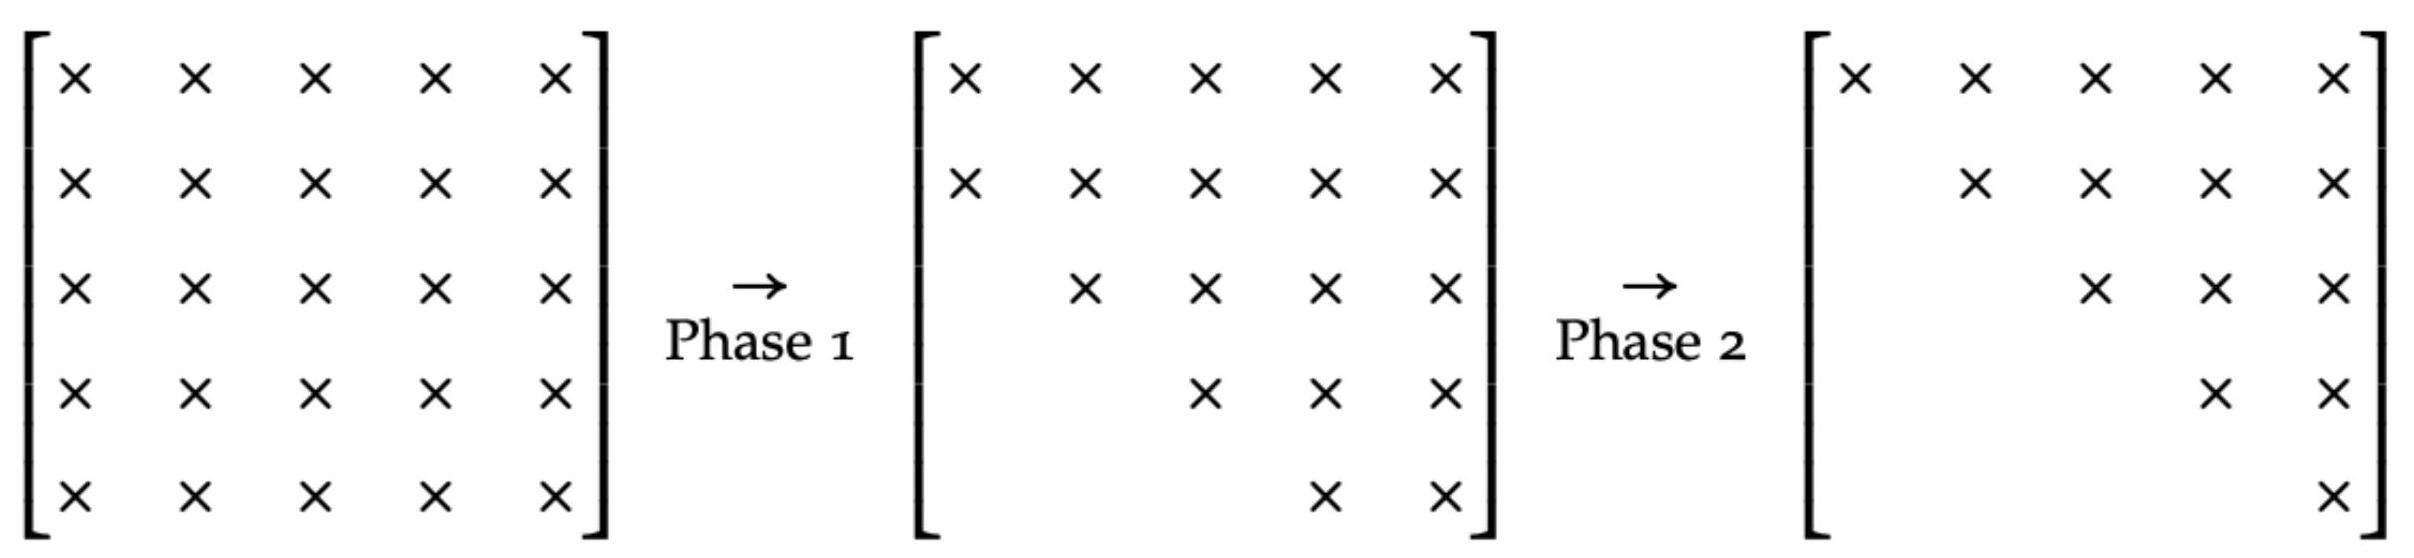
\includegraphics[max width=\textwidth]{2023_09_05_b72ccc85584d9dc6fb5cg-292}
\end{center}

\begin{itemize}
  \item \textbf{Phase 1.} Compute a Hessenberg matrix $H$ (and an orthogonal matrix $U$) such that $A=U H U^{H}$. Such a reduction can be done with a finite number of operations.

  \item \textbf{Phase 2.} Apply the basic QR-method to the matrix $H$. It turns out that when applying the basic QR-method to a Hessenberg matrix the complexity of one step is $O\left(n^{2}\right)$, instead of $O\left(n^{3}\right)$ of the basic version.

\end{itemize}

\section*{The Lanczos algorithm}

The Lanczos algorithm can be used to efficiently find the extremal eigenvalues (maximum and minimum) of a symmetric matrix $A$ of size $n \times n$.
It is based on computing the following decomposition of $A$ :
$$
A=Q T Q^{T}
$$
where $Q$ whose columns is an orthonormal basis of vectors $\mathbf{q}_{1}, \ldots, \mathbf{q}_{n}$ and $T$ is tri-diagonal:
$$
Q=\left[\mathbf{q}_{1}, \mathbf{q}_{2}, \ldots, \mathbf{q}_{n}\right] \quad T=\left[\begin{array}{ccccc}
\alpha_{1} & \beta_{1} & 0 & \ldots & 0 \\
\beta_{1} & \alpha_{2} & \beta_{2} & \ldots & 0 \\
0 & \ddots & \ddots & \vdots & 0 \\
0 & \ddots & \ddots & \vdots & \beta_{n-1} \\
0 & \ldots & 0 & \beta_{n-1} & \alpha_{n}
\end{array}\right]
$$
The decomposition always exists and is unique given that $\mathbf{q}_{1}$ has been specified. We know that $T=Q^{T} A Q$ which gives
$$
\alpha_{k}=\mathbf{q}_{k}^{T} A \mathbf{q}_{k} \quad \beta_{k}=\mathbf{q}_{k+1}^{T} A \mathbf{q}_{k}
$$
The full decomposition is obtained by imposing $A Q=Q T$ :
$$\left[A \mathbf{q}_{1}, A \mathbf{q}_{2}, \ldots, A \mathbf{q}_{n}\right]=\left[\alpha_{1} \mathbf{q}_{1}+\beta_{1} \mathbf{q}_{2}, \beta_{1} \mathbf{q}_{1}+\alpha_{2} \mathbf{q}_{2}+\beta_{2} \mathbf{q}_{3}, \ldots, \ldots, \beta_{n-1} \mathbf{q}_{n-1}+\alpha_{n} \mathbf{q}_{n}\right].$$
At iteration $k$ the algorithm generates intermediate matrices $Q_{k}$ and $T_{k}$ that satisfy $T_{k}=Q_{k}^{T} A Q_{k}$

$$
\begin{aligned}
\mathbf{Q}_{k} & =\left[\begin{array}{llll}
\mathbf{q}_{1} & \mathbf{q}_{2} & \cdots & \mathbf{q}_{k}
\end{array}\right], \\
\mathbf{T}_{k} & =\left[\begin{array}{ccccc}
\alpha_{1} & \beta_{1} & 0 & \cdots & 0 \\
\beta_{1} & \alpha_{2} & \ddots & & \vdots \\
0 & \ddots & \ddots & \ddots & 0 \\
\vdots & & \ddots & \ddots & \beta_{k} \\
0 & \cdots & 0 & \beta_{k} & \alpha_{k}
\end{array}\right]
\end{aligned}
$$
\textbf{Lanczos algorithm}: \\
$\mathbf{q}_{q}=\mathbf{r}_{0} ; \mathbf{q}_{0}=\mathbf{0} ; \beta_{0}=1 ;$

for $(k=1, \ldots, n)$

\begin{itemize}
  \item if $\left(\beta_{k-1}=0\right)$
        break;
  \item end

  \item $\mathbf{q}_{k}=\mathbf{r}_{k-1} / \beta_{k-1}$;

  \item $\alpha_{k}=\mathbf{q}_{k}^{\top} \mathbf{A} \mathbf{q}_{k}$;

  \item $\mathbf{r}_{k}=\left(\mathbf{A}-\alpha_{k}\right) \mathbf{q}_{k}-\beta_{k-1} \mathbf{q}_{k-1}$;

  \item $\beta_{k}=\left|\mathbf{r}_{k}\right|$;

\end{itemize}
end\\ \\ 
\textbf{Remark 1}: $\mathbf{q}_{1}$ is set randomly.\\
\textbf{Remark 2}: The (orthonormal) vectors $\mathbf{q}_{k}$ are called the Lanczos vectors.

\section*{Properties of $\mathbf{q}_{k}$ and $T_{k}$}
At iteration $k$, the $k$-th Lanczos vector $\mathbf{q}_{k}$ is proven to maximise the I.h.s. of
$$
\max _{\mathbf{y} \neq \mathbf{0}} \frac{\mathbf{y}^{T}\left(Q_{k}^{T} A Q_{k}\right) \mathbf{y}}{\mathbf{y}^{T} \mathbf{y}}=\lambda_{1}\left(T_{k}\right) \leq \lambda_{1}(A)=\lambda_{1}(T)
$$
and to simultaneously minimize the I.h.s. of
$$
\min _{\mathbf{y} \neq \mathbf{0}} \frac{\mathbf{y}^{T}\left(Q_{k}^{T} A Q_{k}\right) \mathbf{y}}{\mathbf{y}^{T} \mathbf{y}}=\lambda_{n}\left(T_{k}\right) \geq \lambda_{n}(A)=\lambda_{n}(T)
$$
where $\lambda_{1}(A)$ and $\lambda_{n}(A)$ are the maximum and the minimum eigenvalue of $\mathrm{A}$, respectively.
The extremal eigenvalues of $T_{k}$ progressively become more similar to the ones of $\mathrm{A}$. Thus, the Lanczos algorithm can be used to compute the extremal eigenvalues of a symmetric matrix $A$.
\begin{itemize}
  \item The Lanczos algorithm only requires matrix-vector multiplications with respect to $A$ (matrix free, very useful if $A$ has a sparse form).

  \item The algorithm is very sensitive to round-off problems. The Lanczos vectors $\mathbf{q}_{k}$ loose orthogonality.

  \item The Lanczos algorithm can be used to efficiently find a low-rank approximation of $A$.

\end{itemize}

\chapter{Overdetermined linear systems}
Overdetermined systems have many applications, including many fitting problems.
When the problems are linear there is a very clean and simple way to find the optimum, if we adopt the sum-of-squares error metric.

\section*{Linear regression}

If there were no experimental uncertainty, the model would fit the data exactly. However, since there is noise, the best we can do is minimise the error. The problem is:
$$
\min _{\alpha_{0}, \alpha_{1}} \sum_{i=1}^{m} e_{i}^{2}=\min _{\alpha_{0}, \alpha_{1}} \sum_{i=1}^{m}\left(\alpha_{0}+\alpha_{1} T_{i}-L_{i}\right)^{2}
$$
The above problem is equivalent to the following:
$$
\min \|A \mathbf{\alpha}-\mathbf{b}\|_{2}^{2}
$$
with
$$
A=\left[\begin{array}{cc}
1 & T_{1} \\
1 & T_{2} \\
\vdots & \vdots \\
1 & T_{m}
\end{array}\right], \quad \mathbf{\alpha}=\left[\begin{array}{c}
\alpha_{0} \\
\alpha_{1}
\end{array}\right], \quad \mathbf{b}=\left[\begin{array}{c}
L_{1} \\
L_{2} \\
\vdots \\
L_{m}
\end{array}\right]
$$

\section*{Polynomial regression}
Suppose the model we expect to fit our data pairs $\left(T_{i}, L_{i}\right), i=1, \ldots, m$ is a cubic polynomial rather than a linear one. The hypothesis now is
$L(T)=\alpha_{0}+\alpha_{1} T+\alpha_{2} T^{2}+\alpha_{3} T^{3}$
\begin{center}
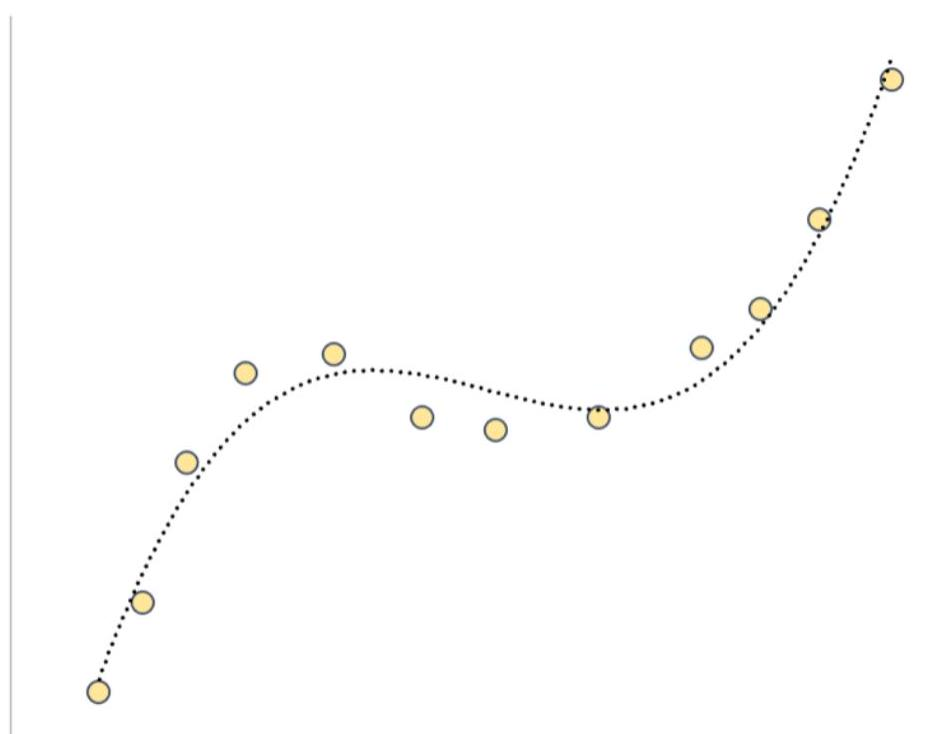
\includegraphics[scale = 0.2]{2023_09_05_b72ccc85584d9dc6fb5cg-304}
\end{center}
The problem now reads:
$$
\min _{\alpha_{0}, \alpha_{1}, \alpha_{2}, \alpha_{3}} \sum_{i=1}^{m} e_{i}^{2}=\min _{\alpha_{0}, \alpha_{1}, \alpha_{2}, \alpha_{3}} \sum_{i=1}^{m}\left(\alpha_{0}+\alpha_{1} T_{i}+\alpha_{2} T_{i}^{2}+\alpha_{3} T_{i}^{3}-L_{i}\right)^{2}
$$

The above problem is equivalent to the following:

$$
\min _{\alpha}\|A \alpha-\mathrm{b}\|_{2}^{2}
$$

with

$$
A=\left[\begin{array}{cccc}
1 & T_{1} & T_{1}^{2} & T_{1}^{3} \\
1 & T_{2} & T_{2}^{2} & T_{2}^{3} \\
\vdots & \vdots & \vdots & \vdots \\
1 & T_{m} & T_{m}^{2} & T_{m}^{3}
\end{array}\right], \quad \alpha=\left[\begin{array}{c}
\alpha_{0} \\
\alpha_{1} \\
\alpha_{2} \\
\alpha_{3}
\end{array}\right], \quad \mathbf{b}=\left[\begin{array}{c}
L_{1} \\
L_{2} \\
\vdots \\
L_{m}
\end{array}\right]
$$


\section*{Some preliminary remarks}
Given $A \in \mathbb{R}^{m \times n}, m \geq n$, and $\mathbf{b} \in \mathbb{R}^{m}$ find $\mathbf{x} \in \mathbb{R}^{n}$ such that $A \mathbf{x}=\mathbf{b}$.\\
We notice that generally the above problem has no solution (in the classical sense) unless the right side $\mathbf{b}$ is an element in the range(A).\\
We need a "new" concept of solution. The basic approach is to look for an $\mathbf{x}$ that makes $A\mathbf{x}$ close to $\mathbf{b}$.


\section*{Solution in the least-square sense}
Given $A \in \mathbb{R}^{m \times n}, m \geq n$, we say that $\mathbf{x}^{*} \in \mathbb{R}^{n}$ is a solution of the linear system $A \mathbf{x}=\mathbf{b}$ in the least-squares sense if $\Phi\left(\mathbf{x}^{*}\right)=\min _{\mathbf{y} \in \mathbb{R}^{n}} \Phi(\mathbf{y})$,
where:
$$\Phi(\mathbf{y})=\|A \mathbf{y}-\mathbf{b}\|_{2}^{2}.$$\\
The problem thus consists of minimising the Euclidean norm of the residual.\\
The solution $\mathbf{x}^{*}$ can be found by imposing the condition that the gradient of the function $\Phi(\cdot)$ must be equal to zero at $\mathbf{x}^{*}$.\\ \\
From the definition we have:
$$
\begin{aligned}
\Phi(\mathbf{y}) & =(A \mathbf{y}-\mathbf{b})^{T}(A \mathbf{y}-\mathbf{b}) = \mathbf{y}^{T} A^{T} A \mathbf{y} - \mathbf{y}^TA^T\mathbf{b}-\mathbf{b}^T A \mathbf{y}+\mathbf{b}^{T} \mathbf{b} =  \\
&= \mathbf{y}^{T} A^{T} A \mathbf{y}- (A\mathbf{y})^T\mathbf{b}  -\mathbf{b}^T A \mathbf{y}+ \mathbf{b}^{T} \mathbf{b}=\mathbf{y}^{T} A^{T} A \mathbf{y}-2 \mathbf{b}^{T} A \mathbf{y}+\mathbf{b}^{T} \mathbf{b}.
\end{aligned}
$$
Therefore:
$$
\nabla \Phi(\mathbf{y})=2 A^{T} A \mathbf{y}-2 A^{T} \mathbf{b}
$$
from which it follows that $\mathbf{x}^{*}$ must be the solution of the square system.
$$
A^{T} A \mathbf{x}^{*}=A^{T} \mathbf{b} \quad \text { System of normal equations }
$$

\section*{Some remarks}
The system of normal equations is non-singular if A has full rank and, in such a case, the least-squares solution exists and is unique.\\
We notice that $B=A^{T} A$ is a symmetric and positive definite matrix.\\
Thus, in order to solve the normal equations, one could first compute the Cholesky factorization $B=R^{T} R$ and then solve the two systems $R^{T} \mathbf{y}=A^{T} \mathbf{y} $ and $ R \mathbf{x}^{*}= \mathbf{y}$.\\ \\
However, $A^{T} A$ is very badly conditioned and, due to round off errors, the computation of $A^{T} A$ may be affected by a loss of significant digits, with a consequent loss of positive definiteness or non-singularity of the matrix.\\
For a matrix A with full rank, the corresponding matrix $\mathrm{fl}\left(A^{T} A\right)$ turns out to be singular.\\
Example:
$$
\mathrm{A}=\left[\begin{array}{cc}
1 & 1 \\
2^{-27} & 0 \\
0 & 2^{-27}
\end{array}\right], f l\left(\mathrm{~A}^{T} \mathrm{~A}\right)=\left[\begin{array}{ll}
1 & 1 \\
1 & 1
\end{array}\right]
$$



\section*{The full QR Factorisation}
Let $A$ be an $m \times n$ matrix. The full QR factorisation of $A$ is the factorisation $A=QR$, where $Q$ is an $m \times m$ orthogonal matrix ($QQ^{T}=I$) and $R$ is an $m \times n$ upper-trapezoidal matrix.\\
On the other hand, the reduced QR factorisation of $A$ is the factorisation $A=\hat{Q}\hat{R}$, where $\hat{Q}$ is an $m \times n$ matrix and $\hat{R}$ is an $n \times n$ upper-triangular matrix. This form of factorisation is often used in numerical linear algebra, as it provides a numerically stable method for solving systems of linear equations, among other applications.\\


\section*{Solution in the least-square sense}
Instead of considering the system of normal equations, we can use the $Q R$ factorisation. The following result holds.\\ \\
\textbf{Theorem:} Let $A \in \mathbb{R}^{m \times n}$, with $m \geq n$, be a full rank matrix. Then the unique solution in the least-square sense $\mathbf{x}^{*}$ of $A \mathbf{x}^{*}=\mathbf{b}$ is given by:
$\mathbf{x}^{*}=\hat{R}^{-1} \hat{Q}^{T} \mathbf{b}$, where $\hat{R} \in \mathbb{R}^{n \times n}$ and $\hat{Q} \in \mathbb{R}^{m \times n}$ are the matrices of the reduced $Q R$ factorisation of $A$. Moreover, the minimum of $\Phi(\cdot)$ is given by:
$$\Phi\left(x^{*}\right)=\sum_{i=n+1}^{m}\left[\left(Q^{T} \mathbf{b}\right)_{i}\right]^{2}$$

\section*{Solution in the least-square sense - proof}
\textbf{Step 1.} The $Q R$ factorization of $A$ exists and is unique since $A$ has full rank. Thus, there exist two matrices, $Q \in \mathbb{R}^{m \times m}$ and $R \in \mathbb{R}^{m \times n}$ such that $A=Q R$, where $Q$ is orthogonal and $R$ is an upper trapezoidal matrix.\\
\textbf{Step 2.} We observe that since $Q$ is an orthogonal matrix $\left(Q^{T} Q=Q Q^{T}=I\right)$ it preserves the Euclidean scalar product, i.e.,
$$
\|Q \mathbf{z}\|_{2}^{2}=(Q \mathbf{z})^{T} Q \mathbf{z}=\mathbf{z}^{T} Q^{T} Q \mathbf{z}=\mathbf{z}^{T} \mathbf{z}=\|\mathbf{z}\|_{2}^{2} \quad \forall \mathbf{z} \in \mathbb{R}^{m}
$$
$\left\|Q^{T} \mathbf{z}\right\|_{2}^{2}=\left(Q^{T} \mathbf{z}\right)^{T} Q^{T} \mathbf{z}=\mathbf{z}^{T} Q Q^{T} \mathbf{z}=\mathbf{z}^{T} \mathbf{z}=\|\mathbf{z}\|_{2}^{2} \quad \forall \mathbf{z} \in \mathbb{R}^{m}$
It follows that:
$$
\|A \mathbf{x}-b\|_{2}^{2}=\left\|Q^{T}(A \mathbf{x}-b)\right\|_{2}^{2}=\left\|Q^{T}(Q R \mathbf{x}-b)\right\|_{2}^{2}=\left\|R \mathbf{x}-Q^{T} b\right\|_{2}^{2} .
$$
Recalling that $\mathrm{R}$ is upper trapezoidal, we have:
$$
\|A \mathbf{x}-b\|_{2}^{2}=\left\|R \mathbf{x}-Q^{T} b\right\|_{2}^{2}=\left\|\hat{R} \mathbf{x}-\hat{Q}^{T} b\right\|_{2}^{2}+\sum_{i=n+1}^{m}\left[\left(Q^{T} b\right)_{i}\right]^{2}.
$$

\section*{If $A$ does not have full rank?}
If $A$ does not have full rank, the above solution techniques above fails.
In this case if $\mathbf{x}^{*}$ is a solution in the least square sense, the vector $\mathbf{x}^{*}+\mathbf{z}$, with $\mathbf{z} \in \operatorname{ker}(A)$, is a solution too.
We must therefore introduce a further constraint to enforce the uniqueness of the solution. Typically, one requires that $\mathbf{x}^{*}$ has minimal Euclidean norm, so that the least-squares problem can be formulated as:\\
Find $\mathbf{x}^{*} \in \mathbb{R}^{n}$ with minimal Euclidean norm such that:
$$\left\|A \mathbf{x}^{*}-\mathbf{b}\right\|_{2}^{2} \leq \min _{\mathbf{x} \in \mathbb{R}^{n}}\|A \mathbf{x}-\mathbf{b}\|_{2}^{2}$$
This problem is consistent with our formulation. If A has full rank, since in this case the solution in the least-square sense exists and is unique it necessarily must have minimal Euclidean norm.
The tool for solving this problem is the singular value decomposition (SVD).

\section*{Singular Value Decomposition (SVD)}
  
Any matrix can be reduced in diagonal form by a suitable pre and postmultiplication by unitary matrices. Precisely, the following result holds.\\ \\
\textbf{Property} Let $\mathrm{A} \in \mathbb{C}^{m \times n}$. There exist two unitary matrices $\mathrm{U} \in \mathbb{C}^{m \times m}$ and $\mathrm{V} \in \mathbb{C}^{n \times n}$ such that
$$
\mathrm{U}^H \mathrm{AV}=\Sigma=\operatorname{diag}\left(\sigma_1, \ldots, \sigma_p\right) \in \mathbb{C}^{m \times n} \quad \text { with } p=\min (m, n)
$$
and $\sigma_1 \geq \ldots \geq \sigma_p \geq 0$. This is called Singular Value Decomposition or ( $S V D$ ) of $\mathrm{A}$ and the numbers $\sigma_i$ (or $\sigma_i(\mathrm{~A})$ ) are called singular values of $\mathrm{A}$.\\ \\
If $\mathrm{A}$ is a real-valued matrix, $\mathrm{U}$ and $\mathrm{V}$ will also be real-valued and $\mathrm{U}^T$ must be written instead of $\mathrm{U}^H$. The following characterization of the singular values holds
$$
\sigma_i(\mathrm{~A})=\sqrt{\lambda_i\left(\mathrm{~A}^H \mathrm{~A}\right)}, \quad i=1, \ldots, n . \ \ (8.1)
$$
Indeed, from the SVD decomposition it follows that $\mathrm{A}=\mathrm{U} \Sigma \mathrm{V}^H, \mathrm{~A}^H=\mathrm{V} \Sigma \mathrm{U}^H$ so that, $\mathrm{U}$ and $\mathrm{V}$ being unitary, $\mathrm{A}^H \mathrm{~A}=\mathrm{V} \Sigma^2 \mathrm{~V}^H$, that is, $\lambda_i\left(\mathrm{~A}^H \mathrm{~A}\right)=\lambda_i\left(\Sigma^2\right)=\left(\sigma_i(\mathrm{~A})\right)^2$. Since $\mathrm{AA}^H$ and $\mathrm{A}^H \mathrm{~A}$ are hermitian matrices, the columns of $\mathrm{U}$, called the left singular vectors of $\mathrm{A}$, turn out to be the eigenvectors of $\mathrm{AA}^H$ and, therefore, they are not uniquely defined. The same holds for the columns of $\mathrm{V}$, which are the right singular vectors of $\mathrm{A}$.\\ \\
Relation (8.1) implies that if $\mathrm{A} \in \mathbb{C}^{n \times n}$ is hermitian with eigenvalues given by $\lambda_1, \lambda_2, \ldots, \lambda_n$, then the singular values of A coincide with the modules of the eigenvalues of $\mathrm{A}$. Indeed because $\mathrm{AA}^H=\mathrm{A}^2, \sigma_i=\sqrt{\lambda_i^2}=\left|\lambda_i\right|$ for $i=1, \ldots, n$. As far as the rank is concerned, if
$$
\sigma_1 \geq \ldots \geq \sigma_r>\sigma_{r+1}=\ldots=\sigma_p=0,
$$
then the rank of A is $r$, the kernel of A is the span of the column vectors of $\mathrm{V},\left\{\mathbf{v}_{r+1}, \ldots, \mathbf{v}_n\right\}$, and the range of $\mathrm{A}$ is the span of the column vectors of $\mathrm{U},\left\{\mathbf{u}_1, \ldots, \mathbf{u}_r\right\}$.\\ \\
\textbf{Definition} Suppose that $\mathrm{A} \in \mathbb{C}^{m \times n}$ has rank equal to $r$ and that it admits a SVD of the type $\mathrm{U}^H \mathrm{AV}=\Sigma$. The matrix $\mathrm{A}^{\dagger}=\mathrm{V} \Sigma^{\dagger} \mathrm{U}^H$ is called the Moore-Penrose pseudo-inverse matrix, being
$$
\Sigma^{\dagger}=\operatorname{diag}\left(\frac{1}{\sigma_1}, \ldots, \frac{1}{\sigma_r}, 0, \ldots, 0\right) .
$$
The matrix $\mathrm{A}^{\dagger}$ is also called the generalized inverse of $\mathrm{A}$ (see Exercise 13). Indeed, if $\operatorname{rank}(\mathrm{A})=n<m$, then $\mathrm{A}^{\dagger}=\left(\mathrm{A}^T \mathrm{~A}\right)^{-1} \mathrm{~A}^T$, while if $n=m=$ $\operatorname{rank}(\mathrm{A}), \mathrm{A}^{\dagger}=\mathrm{A}^{-1}$. 
\section*{Returning to the minimization problem}
$$
\boxed{
\begin{aligned}
& \text { Find } \mathbf{x}^{*} \in \mathbb{R}^{n} \text { with minimal Euclidean norm such that } \\
& \left\|A \mathbf{x}^{*}-\mathbf{b}\right\|_{2}^{2} \leq \min _{\mathbf{x} \in \mathbb{R}^{n}}\|A \mathbf{x}-\mathbf{b}\|_{2}^{2}
\end{aligned}
}
$$
\textbf{Theorem.} Let $A \in \mathbb{R}^{m \times n}$ with SVD given by $A=U \Sigma V^{T}$. Then the unique solution to the minimization problem is:
$$
\mathbf{x}^{*}=A^{\dagger} \mathbf{b}
$$
where $A^{\dagger}$ is the pseudo-inverse of $\mathrm{A}$.\\ \\
\textbf{Proof.} Using the SVD of A, the problem is equivalent to finding $\mathbf{w}=V^{T} \mathbf{x}$ such that $\mathbf{W}$ has minimal Euclidean norm and:
$$
\left\|\Sigma \mathbf{w}-U^{T} \mathbf{b}\right\|_{2}^{2} \leq\left\|\Sigma \mathbf{y}-U^{T} \mathbf{b}\right\|_{2}^{2}, \quad \forall \mathbf{y} \in \mathbb{R}^{n} .
$$
If $r$ is the number of nonzero singular values $\sigma_{i}$ of $\mathrm{A}$, then:
$$
\left\|\Sigma \mathbf{w}-U^{T} \mathbf{b}\right\|_{2}^{2}=\sum_{i=1}^{r}\left(\sigma_{i} w_{i}-\left(U^{T} \mathbf{b}\right)_{i}\right)^{2}+\sum_{i=r+1}^{p}\left(\left(U^{T} \mathbf{b}\right)_{i}\right)^{2}
$$
which is minimum if $\sigma_{i} w_{i}-\left(U^{T} \mathbf{b}\right)_{i}=0 \quad \forall i=1, \ldots, r$. Moreover, it is clear that among the vectors $\mathbf{W}$ of $\mathbb{R}^{n}$ having the first $r$ components fixed, the one with minimal Euclidean norm has the remaining $n-r$ components equal to zero. Thus the solution vector, satisfying both the two previously stated conditions, is $\mathbf{w}^{*}=\Sigma^{\dagger} U^{T} \mathbf{b}$, that is:
$$
\mathbf{x}^{*}=V \Sigma^{\dagger} U^{T} \mathbf{b}=A^{\dagger} \mathbf{b},
$$
where $A^{\dagger}$ is the pseudo-inverse of $A$.

\section*{Computing the SVD}
The SVD can be computed by performing an eigenvalue computation for the normal matrix $A^{T} A$. Indeed, let $U$ and $V$ have column partitions.
$$
U=\left[\mathbf{u}_{1}, \ldots, \mathbf{u}_{m}\right] \quad V=\left[\mathbf{v}_{1}, \ldots, \mathbf{v}_{n}\right]
$$
From the relations
$$
A \mathbf{v}_{\mathbf{j}}=\sigma_{j} \mathbf{u}_{\mathbf{j}}, \quad A^{T} \mathbf{u}_{\mathbf{j}}=\sigma_{j} \mathbf{v}_{\mathbf{j}}
$$
it follows that:
$$
A^{T} A \mathbf{v}_{\mathbf{j}}=\sigma_{j}^{2} \mathbf{v}_{\mathbf{j}}
$$
The QR factorization with column pivoting is not directly used for the eigenvalue problem. It’s used to compute the matrix U in the Singular Value Decomposition (SVD) once we have computed V and $\Sigma$.  

\begin{enumerate}  
\item Compute V and $\Sigma$: This is done by solving the eigenvalue problem for the normal matrix $A^TA$. The eigenvectors of this matrix give us the columns of V, and the square roots of the eigenvalues give us the singular values, which are the diagonal entries of $\Sigma$.  
  
\item Compute U: Once we have V and $\Sigma$, we can compute U using the relation A $v_j = \sigma_j u_j$. This gives us a set of vectors that span the column space of A, but they are not necessarily orthonormal.  
  
\item Apply QR factorization with column pivoting: This step is used to orthonormalize the columns of U. The QR factorization decomposes a matrix into a product of an orthogonal matrix and an upper triangular matrix. When applied to our computed U, it gives us an orthogonal matrix whose columns are orthonormal vectors spanning the same space as the original vectors. The column pivoting is used for numerical stability, ensuring that we avoid dividing by small numbers.  
\end{enumerate}  
When you have very small singular values, squaring them (as you might do when working with the normal matrix $A^TA$ in SVD) can lead to even smaller numbers. This can cause problems in numerical computations due to the limitations of floating-point precision, leading to large errors or instability. A possible remedy is to proceed in two steps.\\ \\
The first step uses Householder reflections to reduce the matrix $A \in \mathbb{R}^{m \times n}$, for $m \geq n$, to a bidiagonal form:
$$
A=U B V^T, \quad U \in \mathbb{R}^{m \times m} \text {, } B \in \mathbb{R}^{m \times n}, \quad V \in \mathbb{R}^{n \times n},
$$
where $U$ is orthonormal, $V$ is orthogonal and $B$ is bidiagonal
$$
B=\left[\begin{array}{ccccc}
\psi_1 & \phi_2 & & & \\
& \psi_2 & \phi_3 & & \\
& & \ddots & \ddots & \\
& & & \psi_{n-1} & \phi_n \\
& & & & \psi_n
\end{array}\right] .
$$
This process is called bidiagonalization. The second step is the application of a fast algorithm for computing the singular value decomposition of a bidiagonal matrix.
It follows that $T=B^{T} B$ is symmetric and tridiagonal.\\
We could then apply the (symmetric) QR algorithm directly to T.\\ \\
After bidiagonalization, SVD of the bidiagonal matrix has to be performed to complete the task of computing the singular value decomposition of a general matrix:
$$
B=U_B \Sigma V_B^T .
$$
The final singular value decomposition is then achieved by:
$$
A=\left(U U_B\right) \Sigma\left(V V_B\right)^T.
$$
\\ \\The singular value decomposition (SVD) is an alternative to the eigenvalue decomposition that is better for rank-defficient and ill-conditioned matrices in general.
\section*{Summary}
\begin{itemize}
  \item Computing the SVD is always numerically stable for any matrix, but is typically more expensive than other decompositions.

  \item The SVD can be used to compute low-rank approximations to a matrix via the principal component analysis (PCA) (not discussed).

  \item PCA has many practical applications and usually large sparse matrices appear.

\end{itemize}

\end{document}